\chapter{Final results}
Bottomonium suppression in PbPb collisions is studied in this section by measuring the ratios of observed yields of excited $\PgU$ states relative to the ground $\PgUa$ state, with the $150 \mu b^{-1}$ 2011 \PbPb\ data. The suppression is inferred by performing a comparison of the ratios measured in PbPb against the \pp\ reference. Dependencies on the centrality of the  \PbPb collision are explored. 

The data samples,  reconstruction and selection criteria are described in Sections~\ref{sec:datasets} and~\ref{sec:selection}. 
%
The parameters of interest are extracted from the data samples directly via an extended unbinned maximum likelihood fit to the dimuon invariant-mass spectra, described in Section~\ref{sec:fitting}.


\subsection{Single ratio measurement}
\label{sec:singleratio}

The following ratios of observed yields of $\PgU$ excited states relative to the ground state are studied:
%
\begin{linenomath}
\begin{eqnarray}
\label{eqn:def:r23}
R_{23} & \equiv & \frac{N\left(\PgUb+\PgUc\right)}{N(\PgUa)} \,,\\
\label{eqn:def:r2}
R_{2}  & \equiv & \frac{N\left(\PgUb      \right)}{N(\PgUa)} \,, \\
\label{eqn:def:r3}
R_{3}  & \equiv & \frac{N\left(\PgUc      \right)}{N(\PgUa)} \,.
\end{eqnarray}
\end{linenomath}
%
In addition to the combined excited-to-ground ratio, $R_{23}$, the current statistics allow to extract the separate 2S and 3S ratios, $R_{2}$ and $R_3$. 
No evidence for the $\PgUc$ state is found in the \PbPb data, and the corresponding ratio is studied in Sec.~\ref{sec:limits}. 

These ratios are measured from fits to the PbPb and \Pp\Pp{} datasets, separately performed. 
The nominal $\pt>4.0 \GeVc$ cut is used.
%\footnote{Fit results with $\pt>3.5 \GeVc$ single-muon cut are collected in Appendix~\ref{sec:newdata150}.}
These fits are displayed in \fig{fig:final_massfit_nominal}.
%{fig:massfit_singlerat_pbpb_nominal} and~\ref{fig:massfit_singlerat_pp_nominal}. 
The fit results are shown in Table~\ref{tab:single-rat} for the PbPb data, and in Table~\ref{tab:single-rat-pp} for the \pp\ (2.76 TeV) dataset. 

\begin{figure}[hbtp]
  \begin{center}
    \subfigure[Fit to the PbPb data]{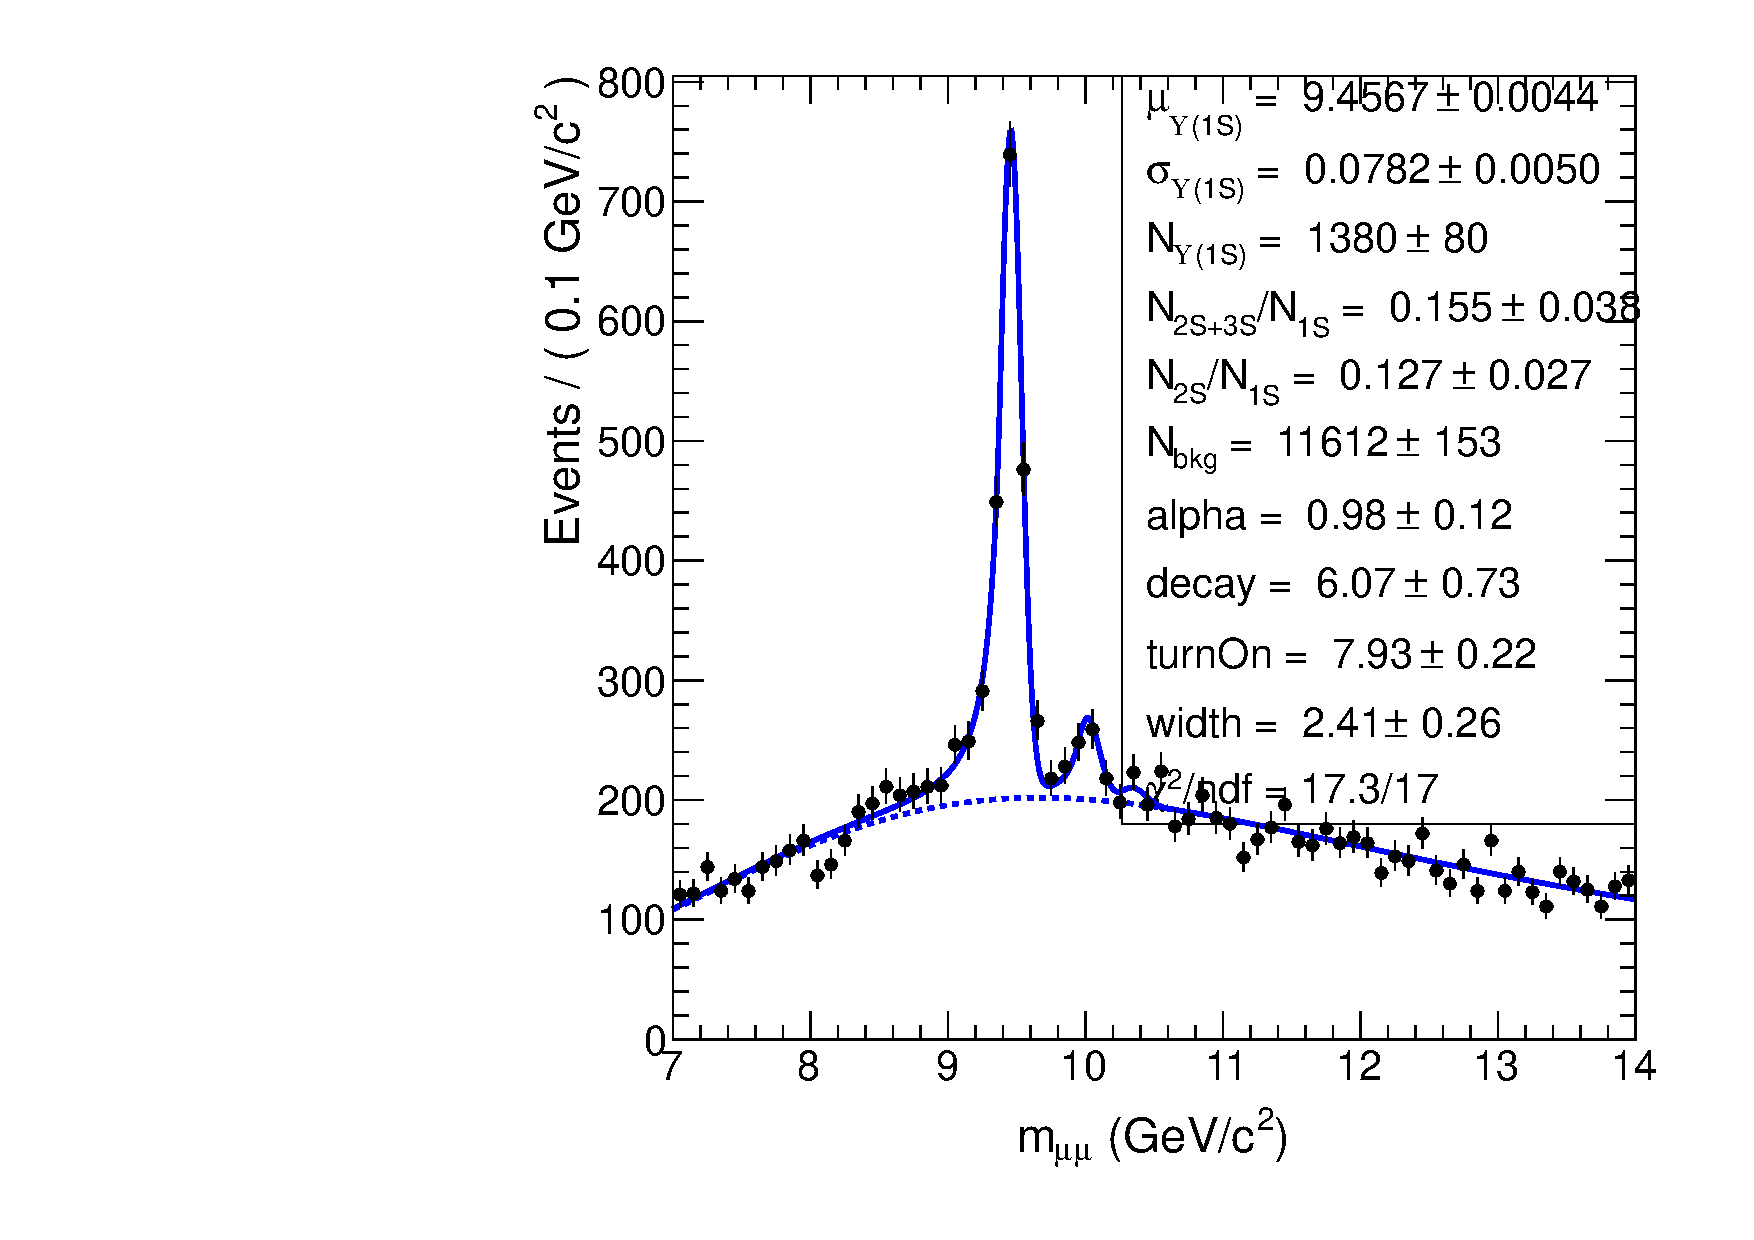
\includegraphics[angle=0,width=0.5\textwidth]{figures/fulldataset/masspeak_Hi_paramOn.pdf}\label{fig:final_massfit_PbPb}}
    \subfigure[Fit to the pp data]{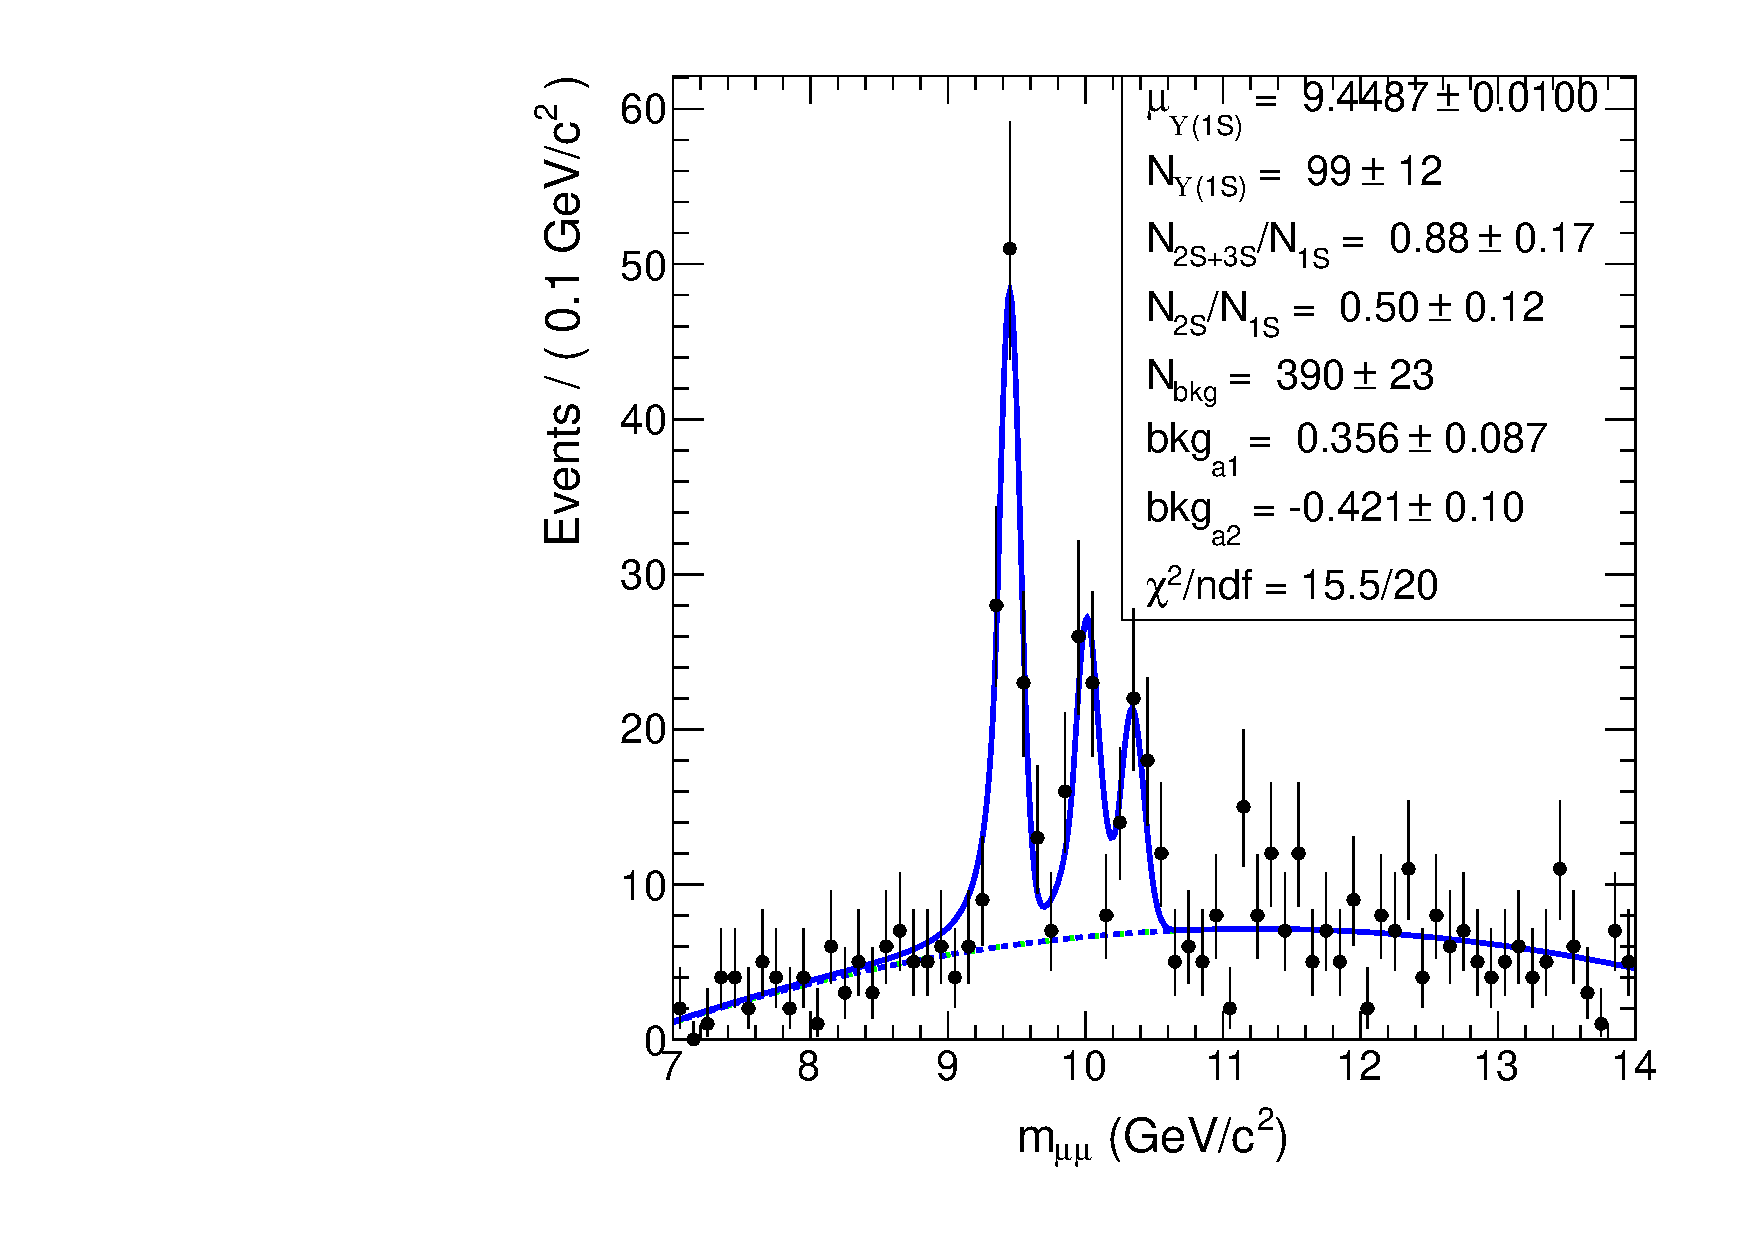
\includegraphics[angle=0,width=0.5\textwidth]{figures/fulldataset/masspeak_pp_HIrereco_pol2_fix_paramOn.pdf}\label{fig:final_massfit_pp}} \\
  \caption{Nominal mass fits, performed separately to the \PbPb ($150 \mu b^{-1}$)  and \pp ($231 nb^{-1}$) full datasets.}
  \label{fig:final_massfit_nominal}
  \end{center}
\end{figure}


Various systematic variations of the fit model are performed, to further establish the stability of the results. 
For the fit to the PbPb data, the following variations are considered:
\begin{itemize}
\item like-sign background modeling: the background model is formed of two components, given by the like-sign distribution and a second order polynomial; the PDF from the like-sign data is obtained from a fit employing the erf * exp model (Fig~\ref{fig:final_PbPb_LSerf}) 
\item like-sign background modeling: the background model is formed of two components, given by the like-sign distribution and a second order polynomial; the PDF from the like-sign data is obtained from the RooKeysPdf smoothing method (Fig~\ref{fig:final_PbPb_LSkeys})
%\item narrow range mass fit (8.5 -- 14 \GeVcc), fitted with second order polynomial (Fig~\ref{fig:final_PbPb_pol2})
%\item narrow range mass fit (8.5 -- 14 \GeVcc), fitted with  first order polynomial (Fig~\ref{fig:final_PbPb_pol1})
\item track-rotation background modeling: the background model is formed of two components, given by the track-rotation distribution and a second order polynomial; the PDF from the track-rotation data is obtained from a fit employing the erf * exp model (Fig~\ref{fig:final_PbPb_TRerf} and~\ref{fig:final_PbPb_TRerf_OS})
\item track-rotation background modeling: the background model is formed of two components, given by the track-rotation distribution and a second order polynomial; the PDF from the track-rotation data is obtained from the RooKeysPdf smoothing method (Fig~\ref{fig:final_PbPb_TRkeys} and~\ref{fig:final_PbPb_TRkeys_OS})
\item the CB signal tail parameters are fixed ($\alpha=1.4$, from high-statistics $\Pp\Pp$ data as in Table~\ref{tab:fsr}) (Fig~\ref{fig:final_PbPb_CBfix}) %, $\sigma_{1S}=92\MeVcc)$
\item the resolution is fixed ($\sigma_{1S}=92\MeVcc$) (Fig~\ref{fig:final_PbPb_resolfix})
%\item wide range mass fit (6 -- 15 \GeVcc), using nominal model (this variations is provided only as a check, given below 7\GeVcc the background model does not provide an appropriate discription of the data)
\item the signal shape parameters are fixed ($\alpha=1.4$, $n=2.3$, $\sigma_{1S}=92\MeVcc$) (Fig~\ref{fig:final_PbPb_CBresolfix})
\end{itemize}

For the fit to the pp data, these variations are considered:
\begin{itemize}
\item the CB signal tail parameters are fixed ($\alpha=1.4$, from high-statistics $\Pp\Pp$ data as in Table~\ref{tab:fsr})  %, $\sigma_{1S}=92\MeVcc)$
\item the resolution is fixed ($\sigma_{1S}=92\MeVcc$) 
\item the signal shape parameters are fixed ($\alpha=1.4$, $n=2.3$, $\sigma_{1S}=92\MeVcc$) 
\item like-sign background modeling: the background model is formed of two components, given by the like-sign distribution and a second order polynomial; the PDF from the like-sign data is obtained from a fit employing the erf * exp model
\item like-sign background modeling: the background model is formed of two components, given by the like-sign distribution and a second order polynomial; the PDF from the like-sign data is obtained from the RooKeysPdf smoothing method
\item error function for background shape
\end{itemize}
%
%For each case, the largest variation observed is assigned as the systematic uncertainty on the measurement. 

\begin{figure}[hbtp]
  \begin{center}
    \subfigure[fix CB to MC (alpha = 1.4)]{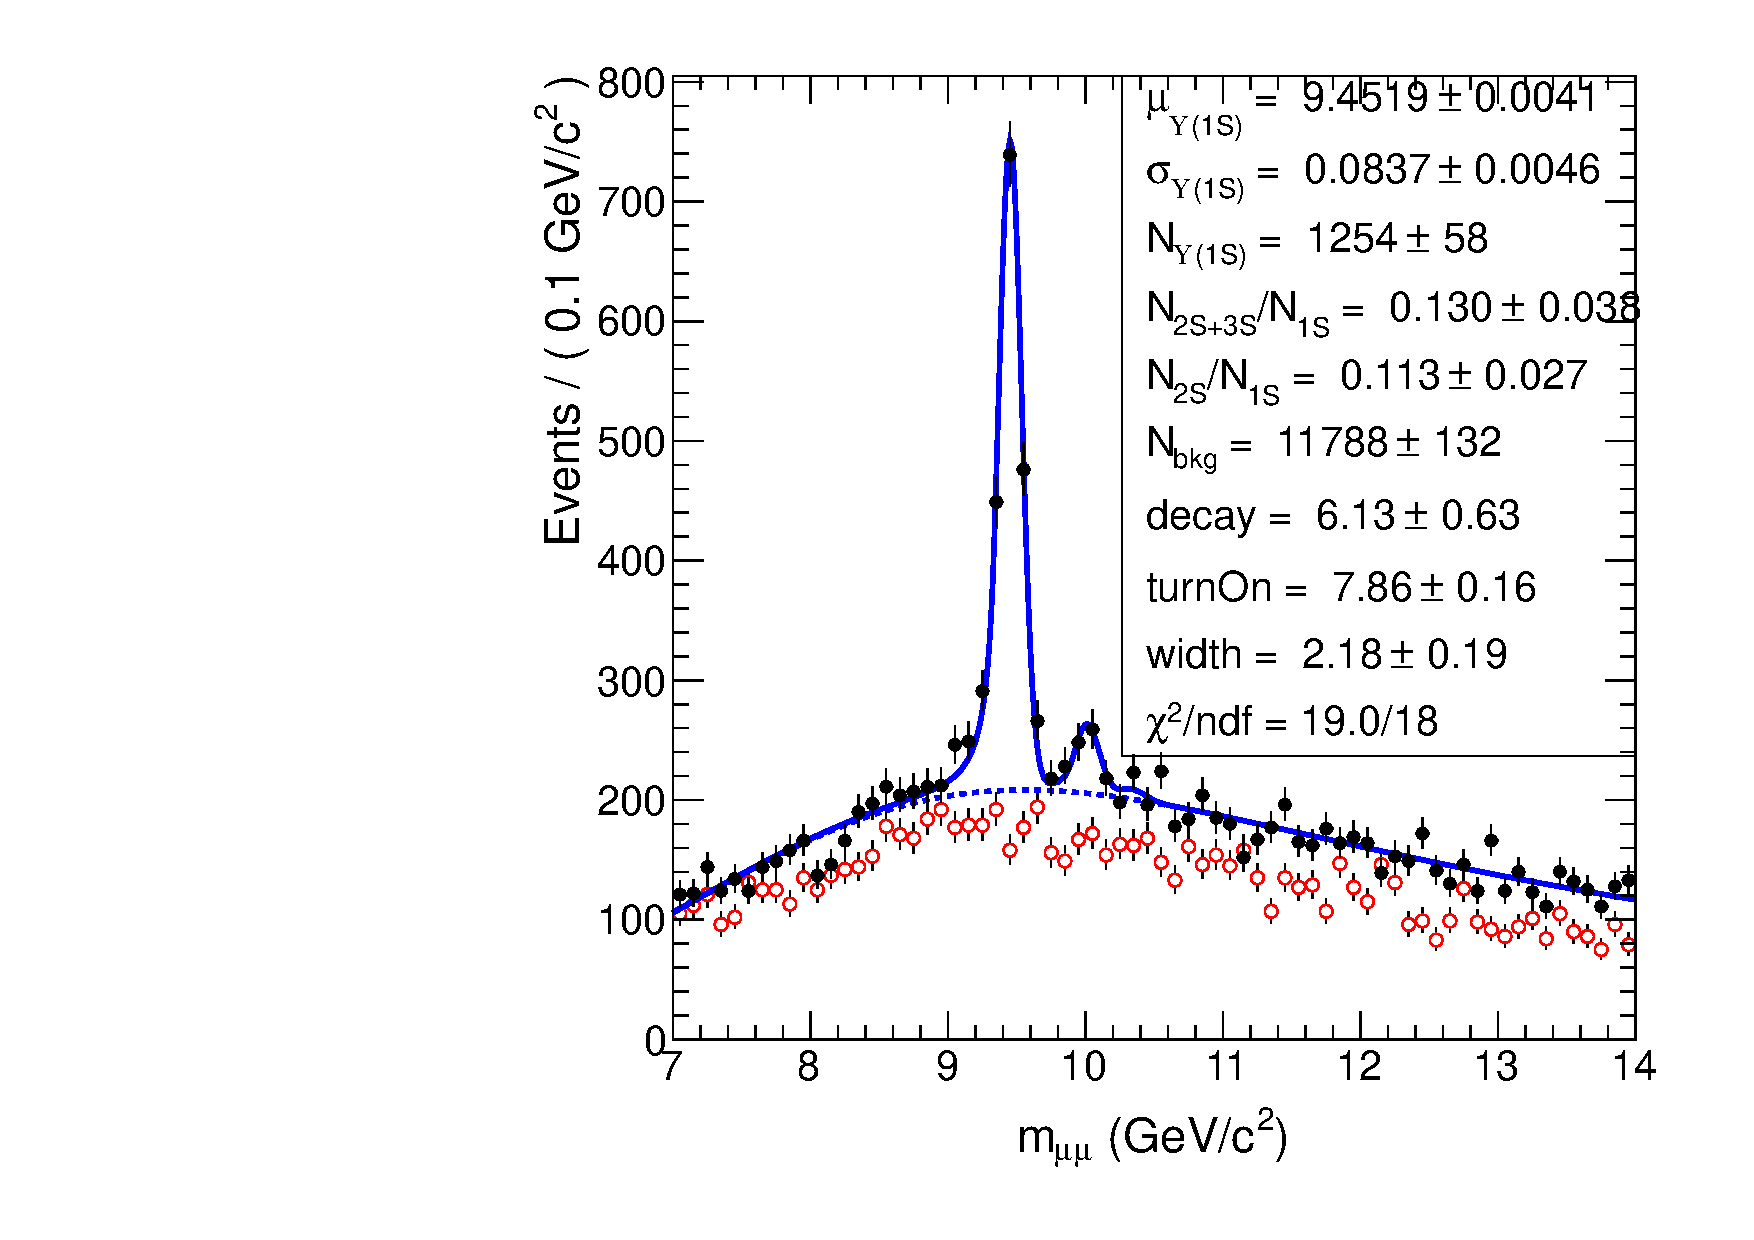
\includegraphics[angle=0,width=0.3\textwidth]{figures/fulldataset/masspeak_hi_CBfix.pdf}\label{fig:final_PbPb_CBfix}}
    \subfigure[fix resolution to MC]{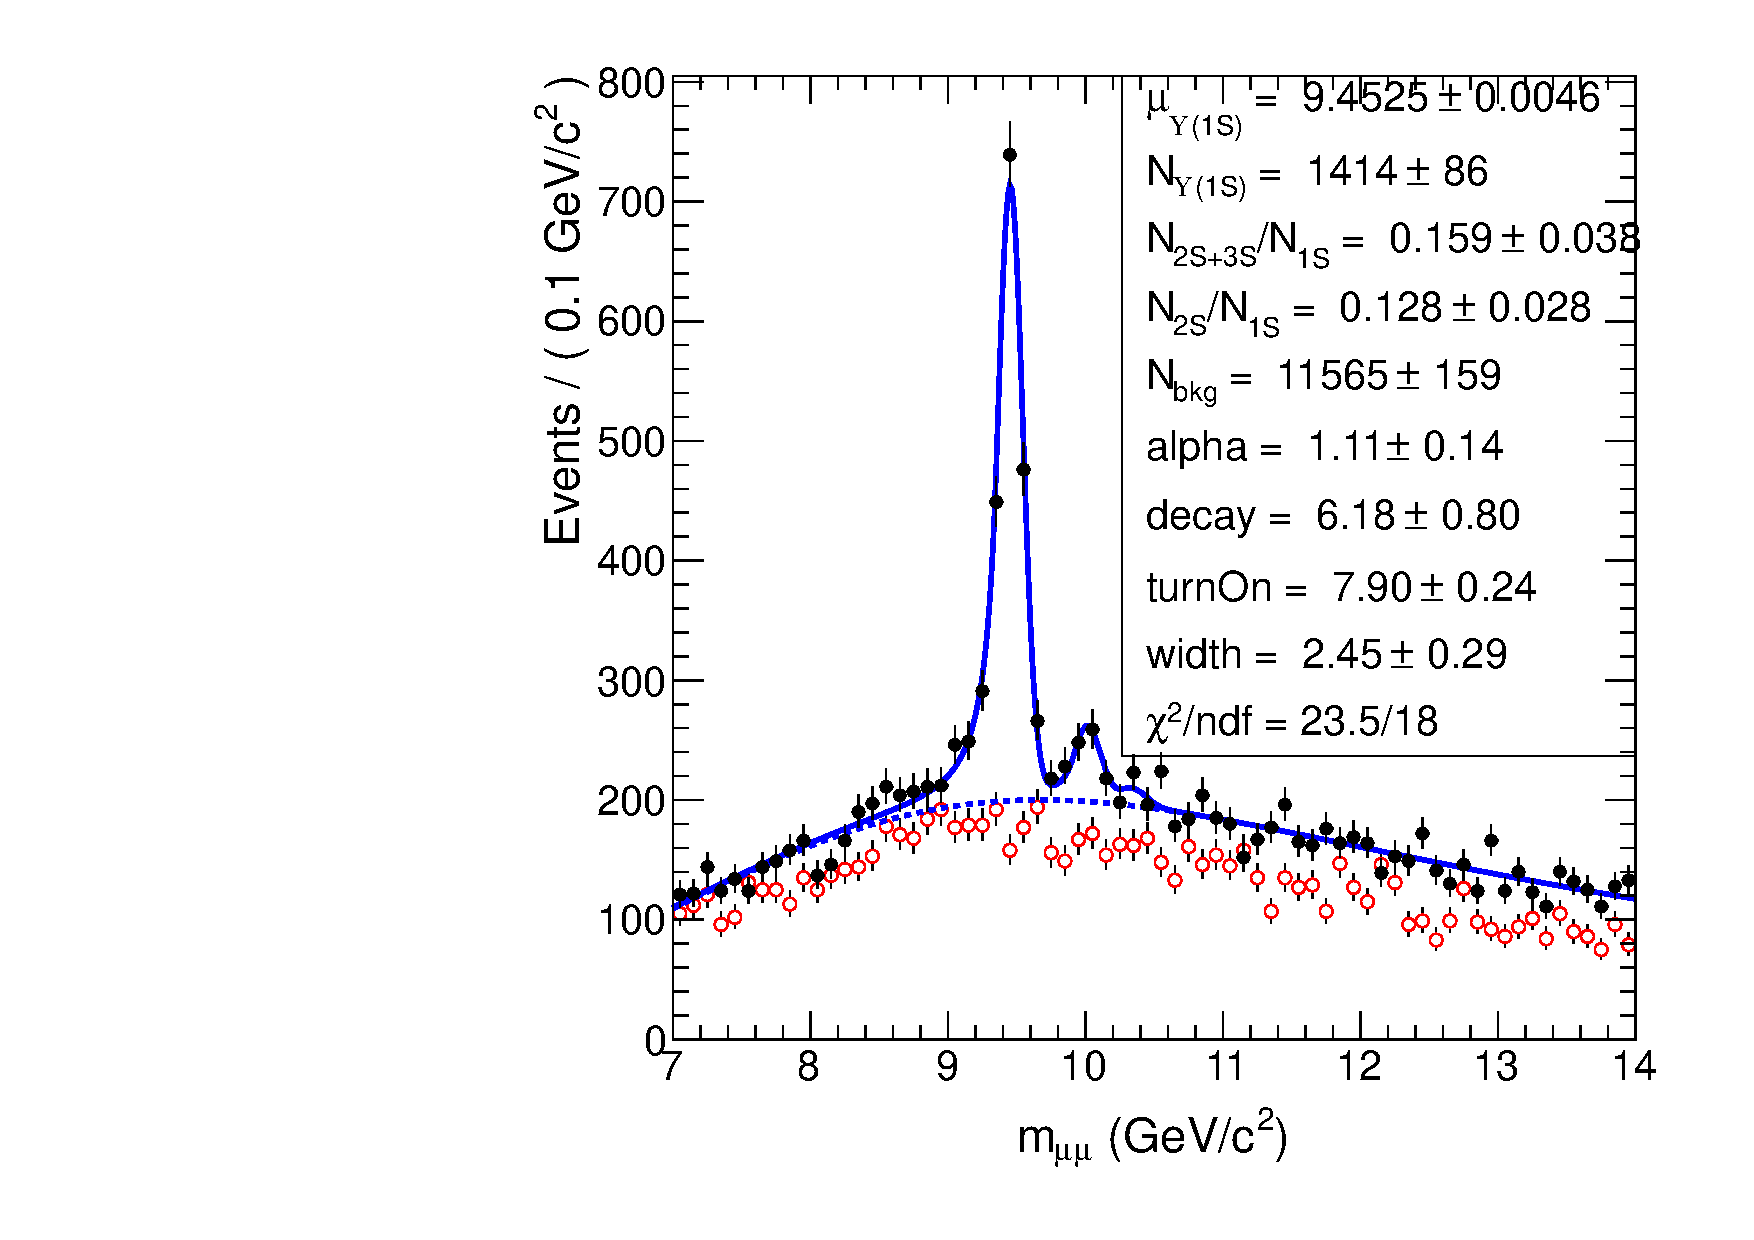
\includegraphics[angle=0,width=0.3\textwidth]{figures/fulldataset/masspeak_hi_resol_fix.pdf}\label{fig:final_PbPb_resolfix}}
    \subfigure[fix CB and resolution to MC]{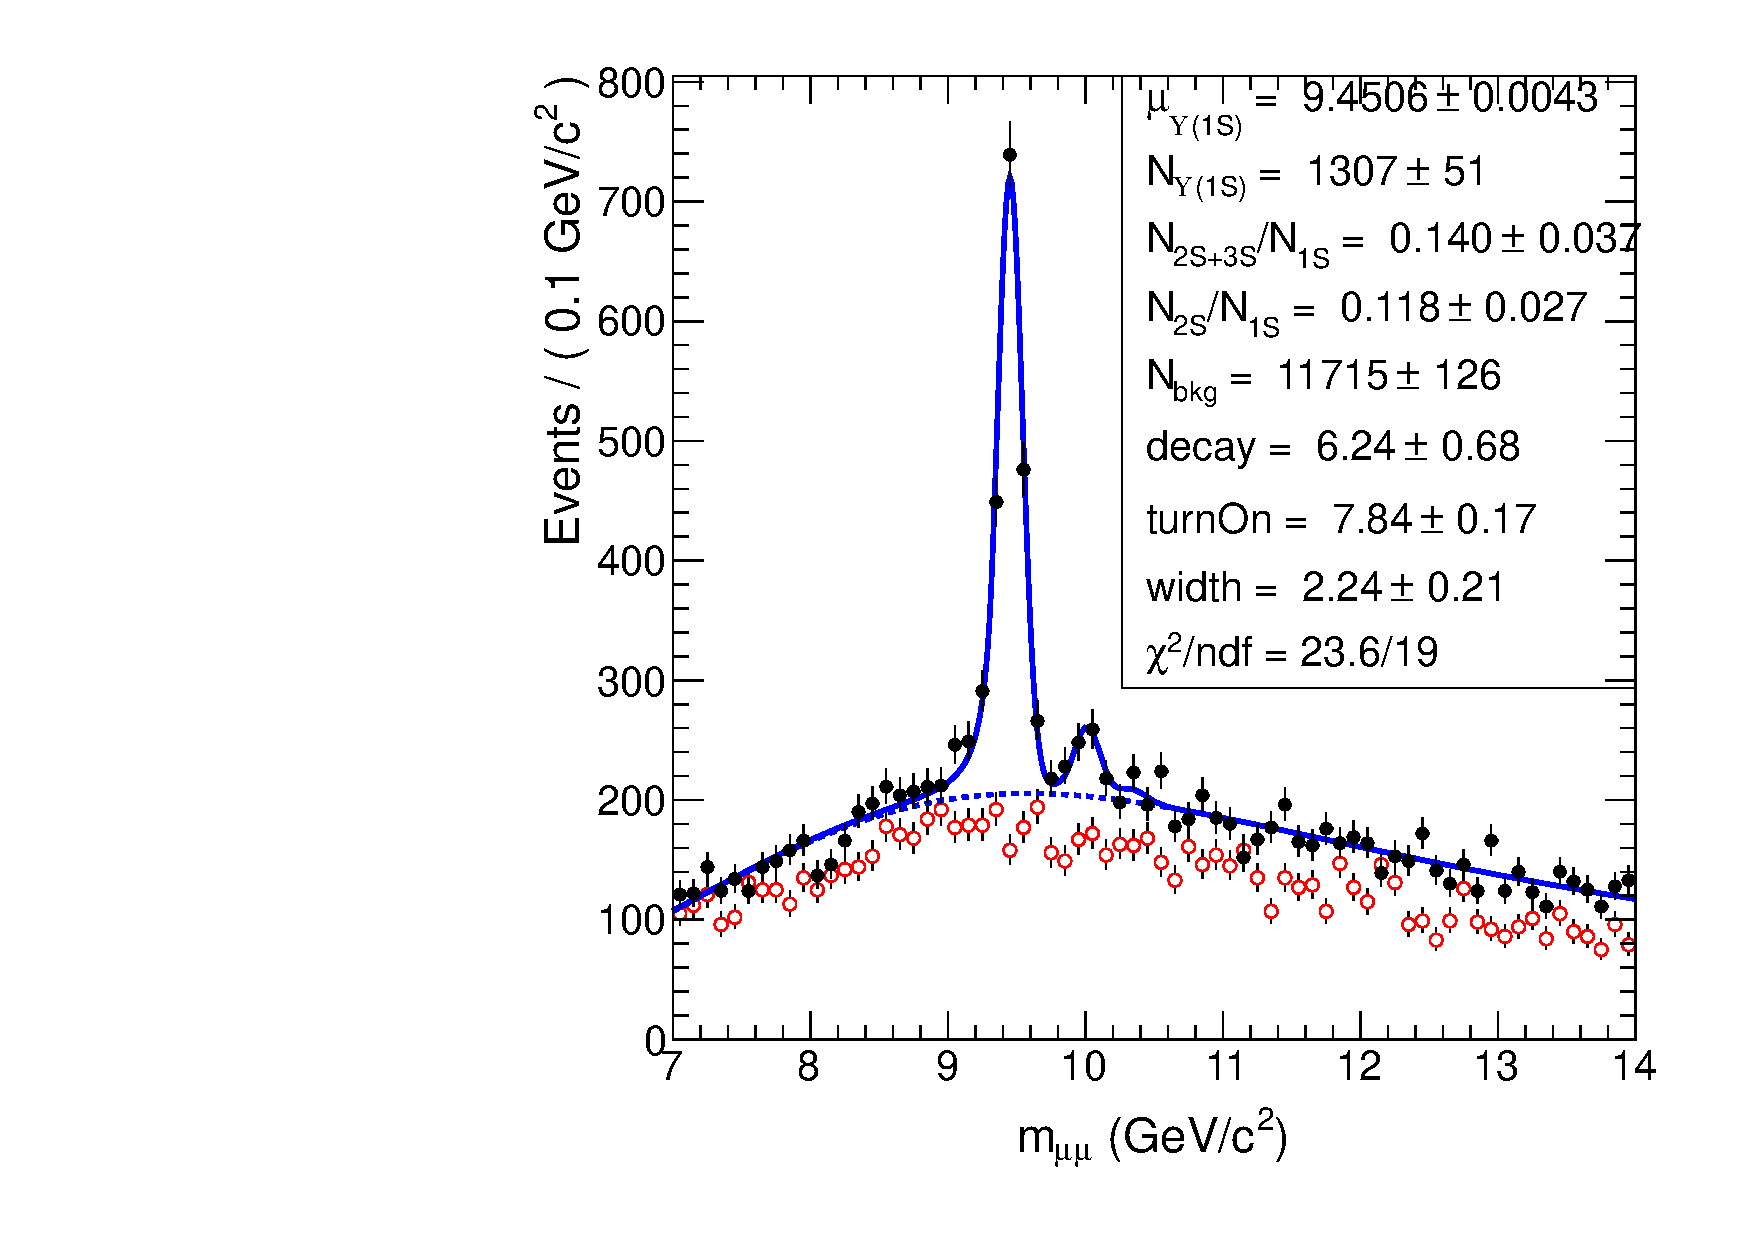
\includegraphics[angle=0,width=0.3\textwidth]{figures/fulldataset/masspeak_hi_resolCB_fix.pdf}\label{fig:final_PbPb_CBresolfix}}\\ 
    \subfigure[LS keys + pol2]{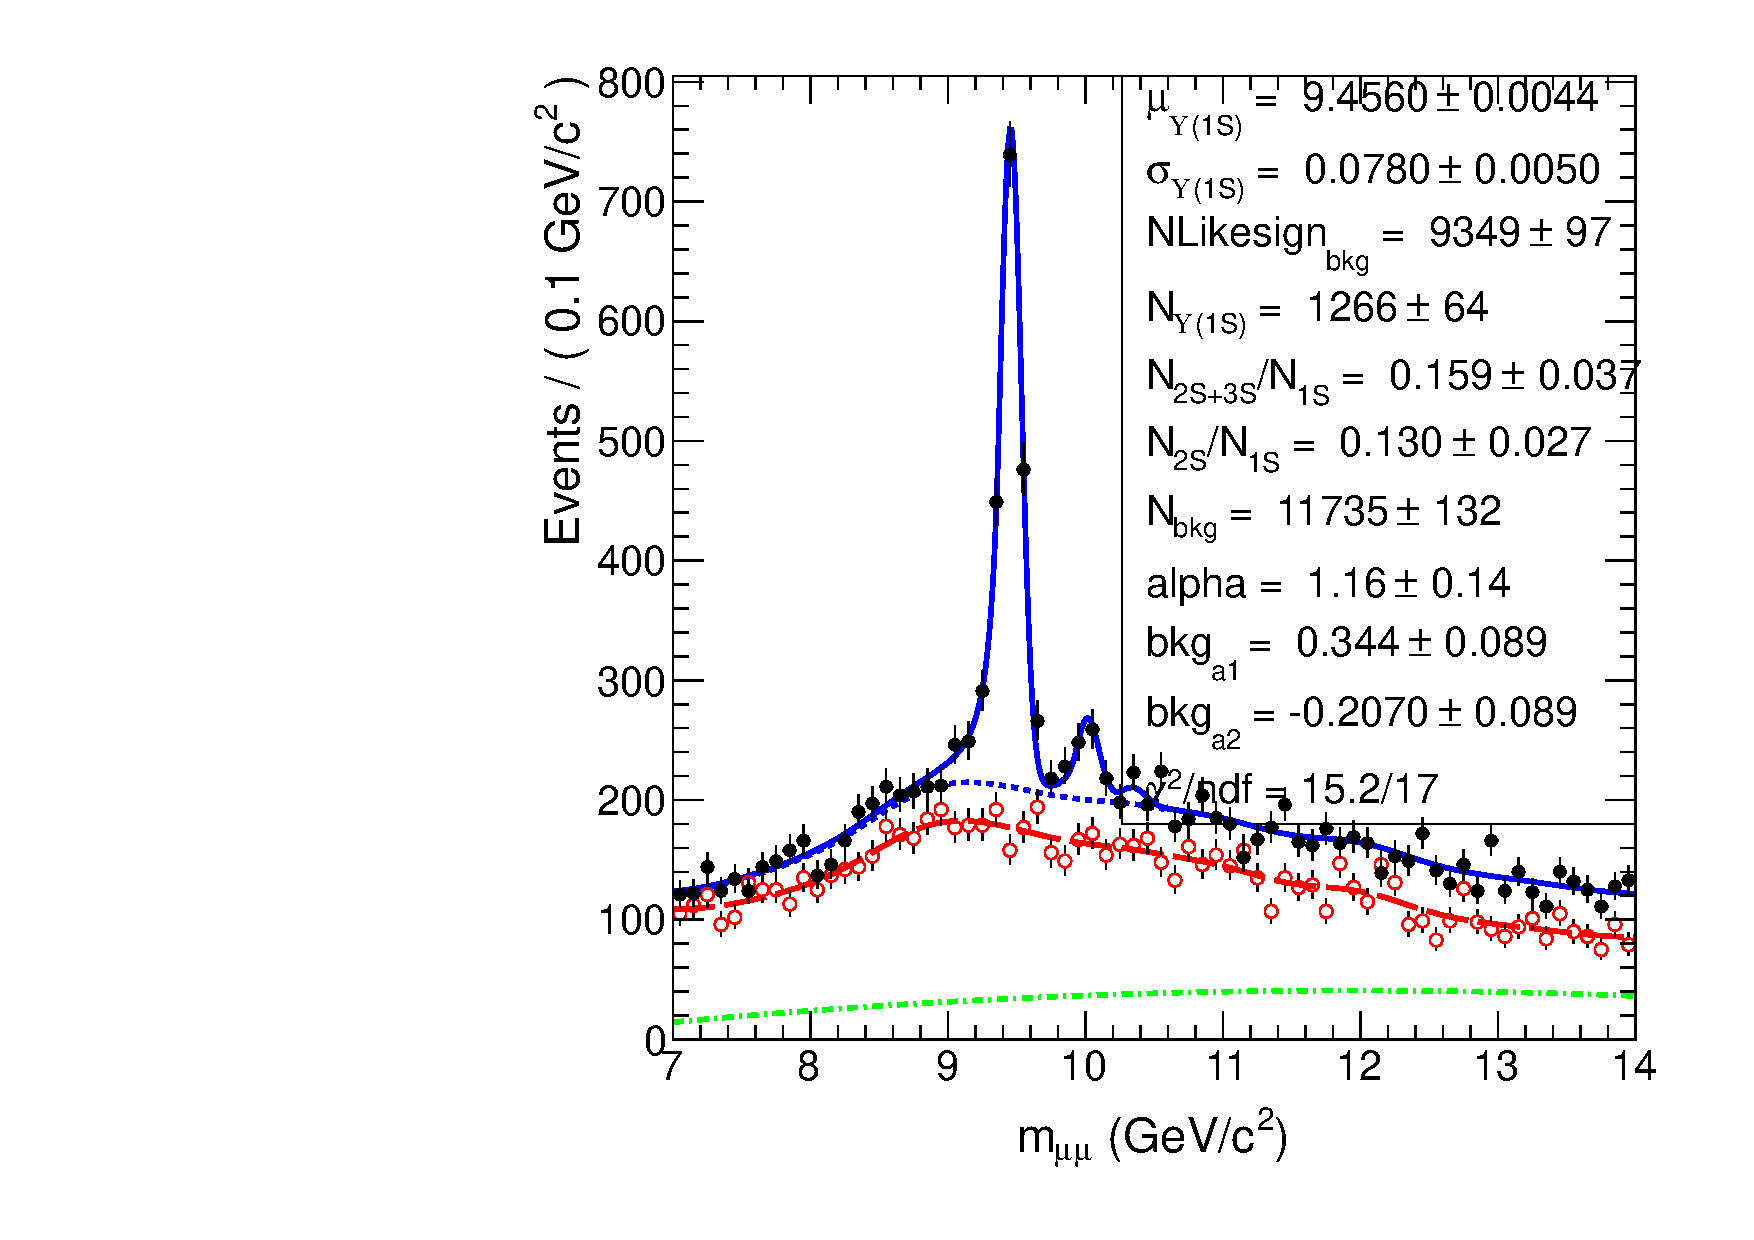
\includegraphics[angle=0,width=0.3\textwidth]{figures/fulldataset/masspeak_hi_LSkeys.pdf}\label{fig:final_PbPb_LSkeys}}
    \subfigure[LS TrkRot keys + pol2]{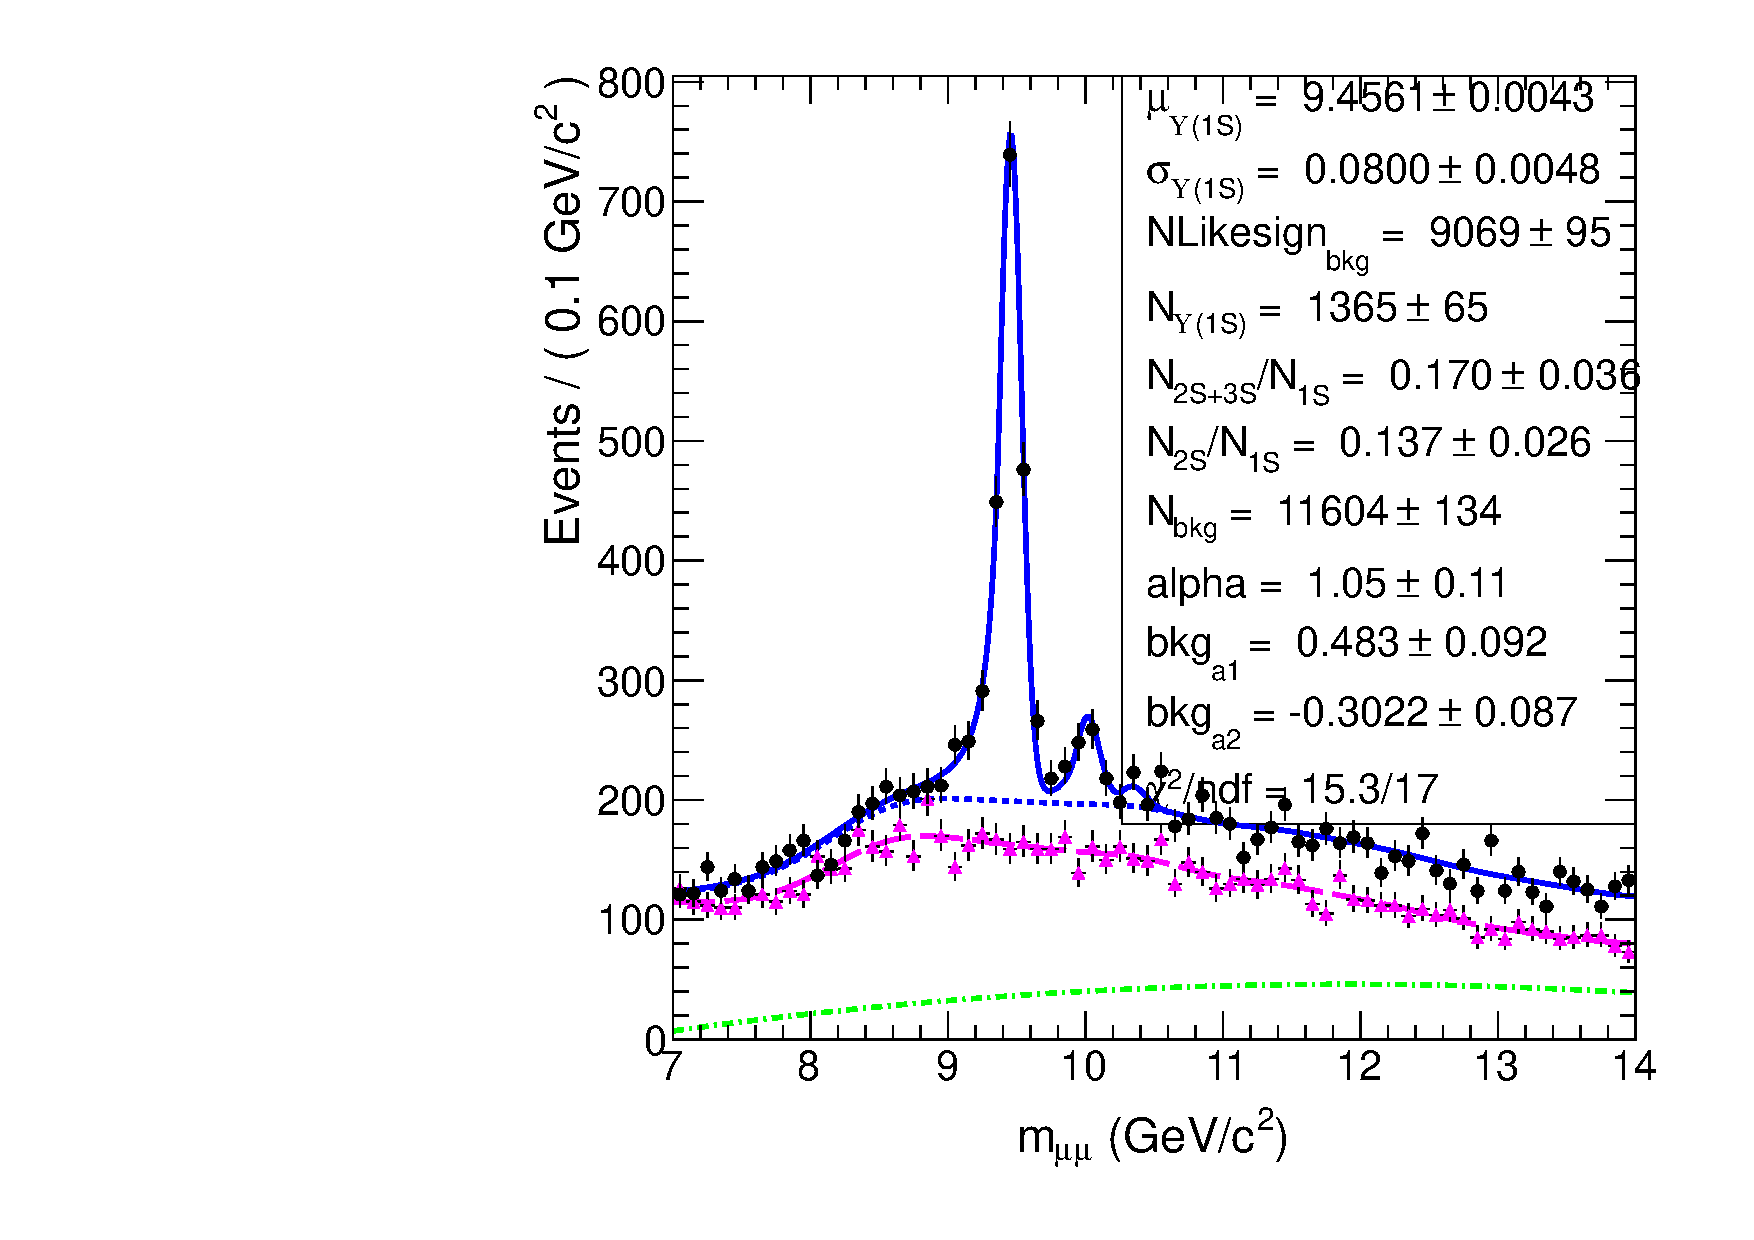
\includegraphics[angle=0,width=0.3\textwidth]{figures/fulldataset/masspeak_hi_TRkeys.pdf}\label{fig:final_PbPb_TRkeys}}
    \subfigure[OS TrkRot keys + pol2]{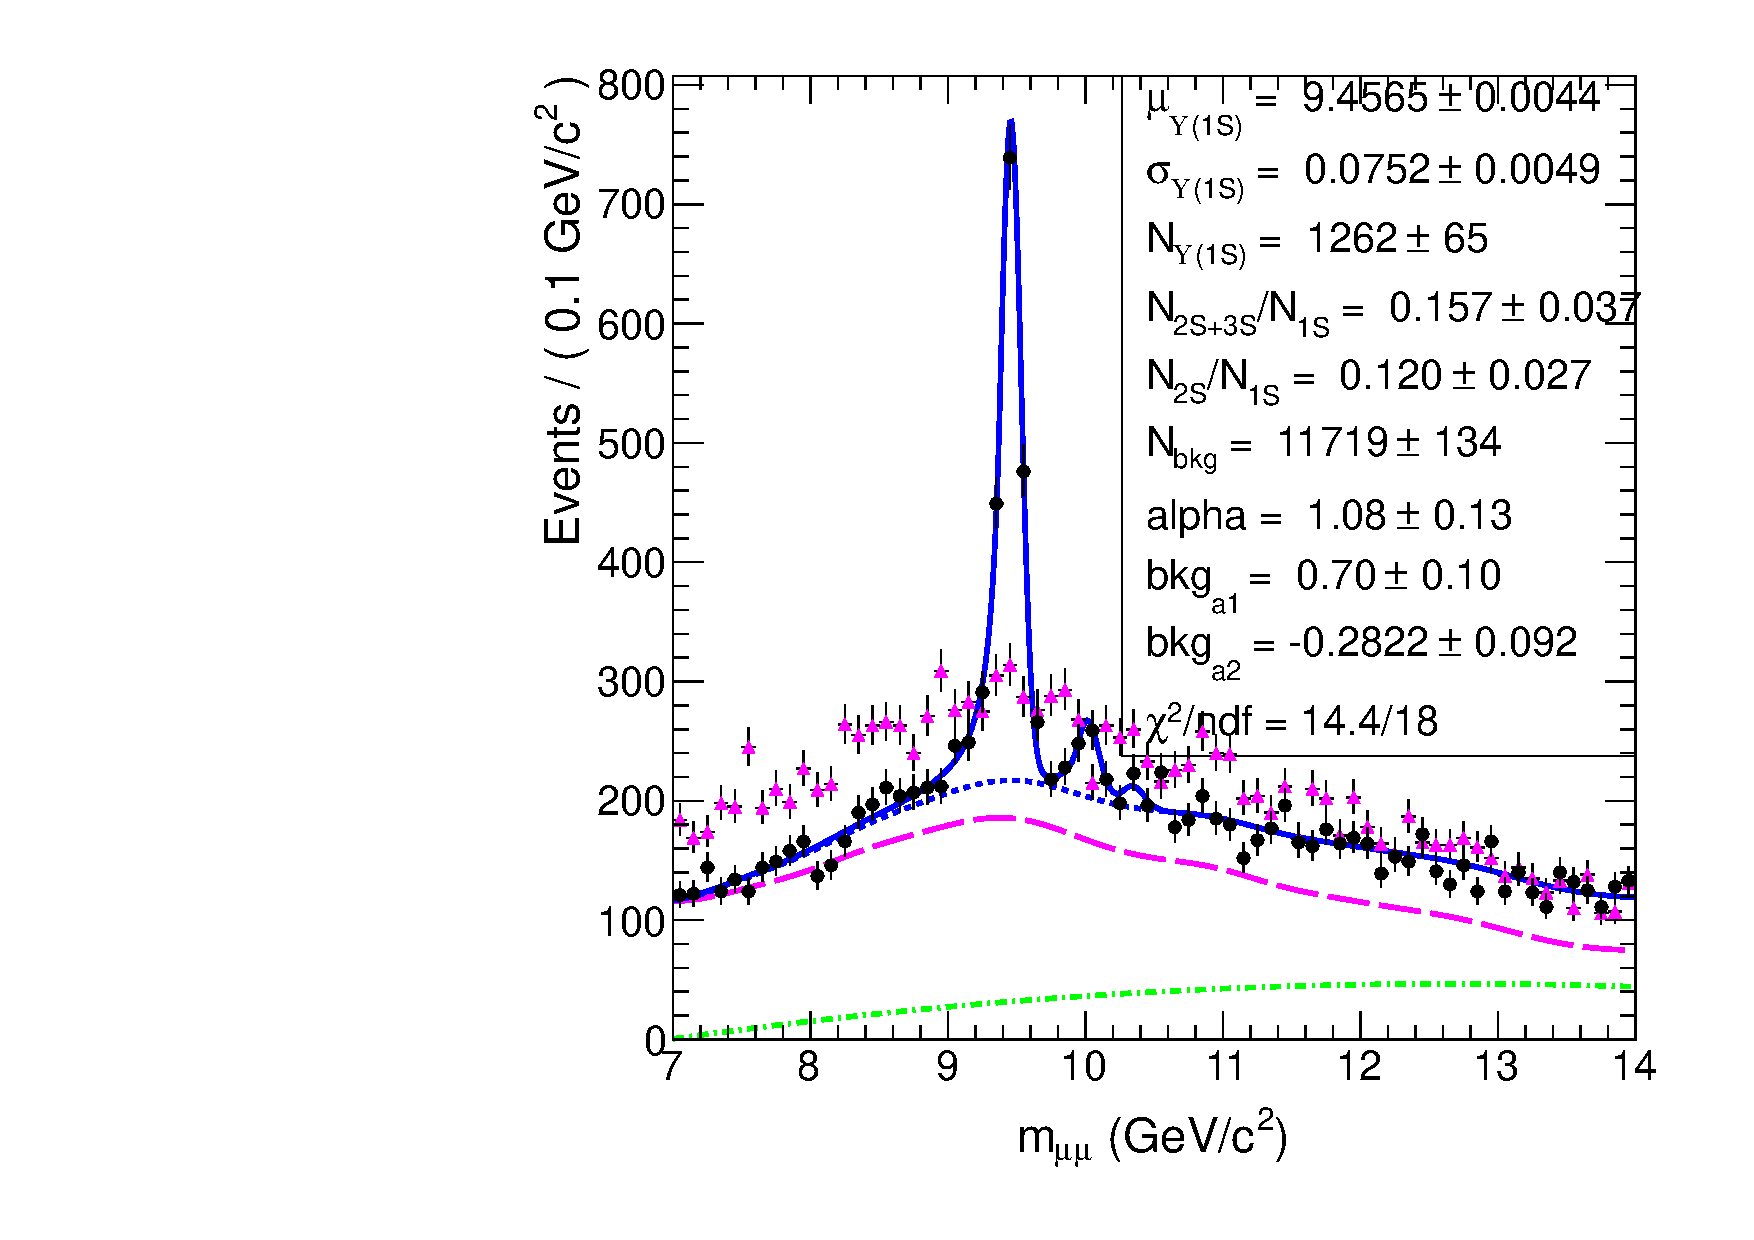
\includegraphics[angle=0,width=0.3\textwidth]{figures/fulldataset/masspeak_Hi_keysPdf_OS_trkRot.pdf}\label{fig:final_PbPb_TRkeys_OS}}\\
    \subfigure[LS erf*exp + pol2]{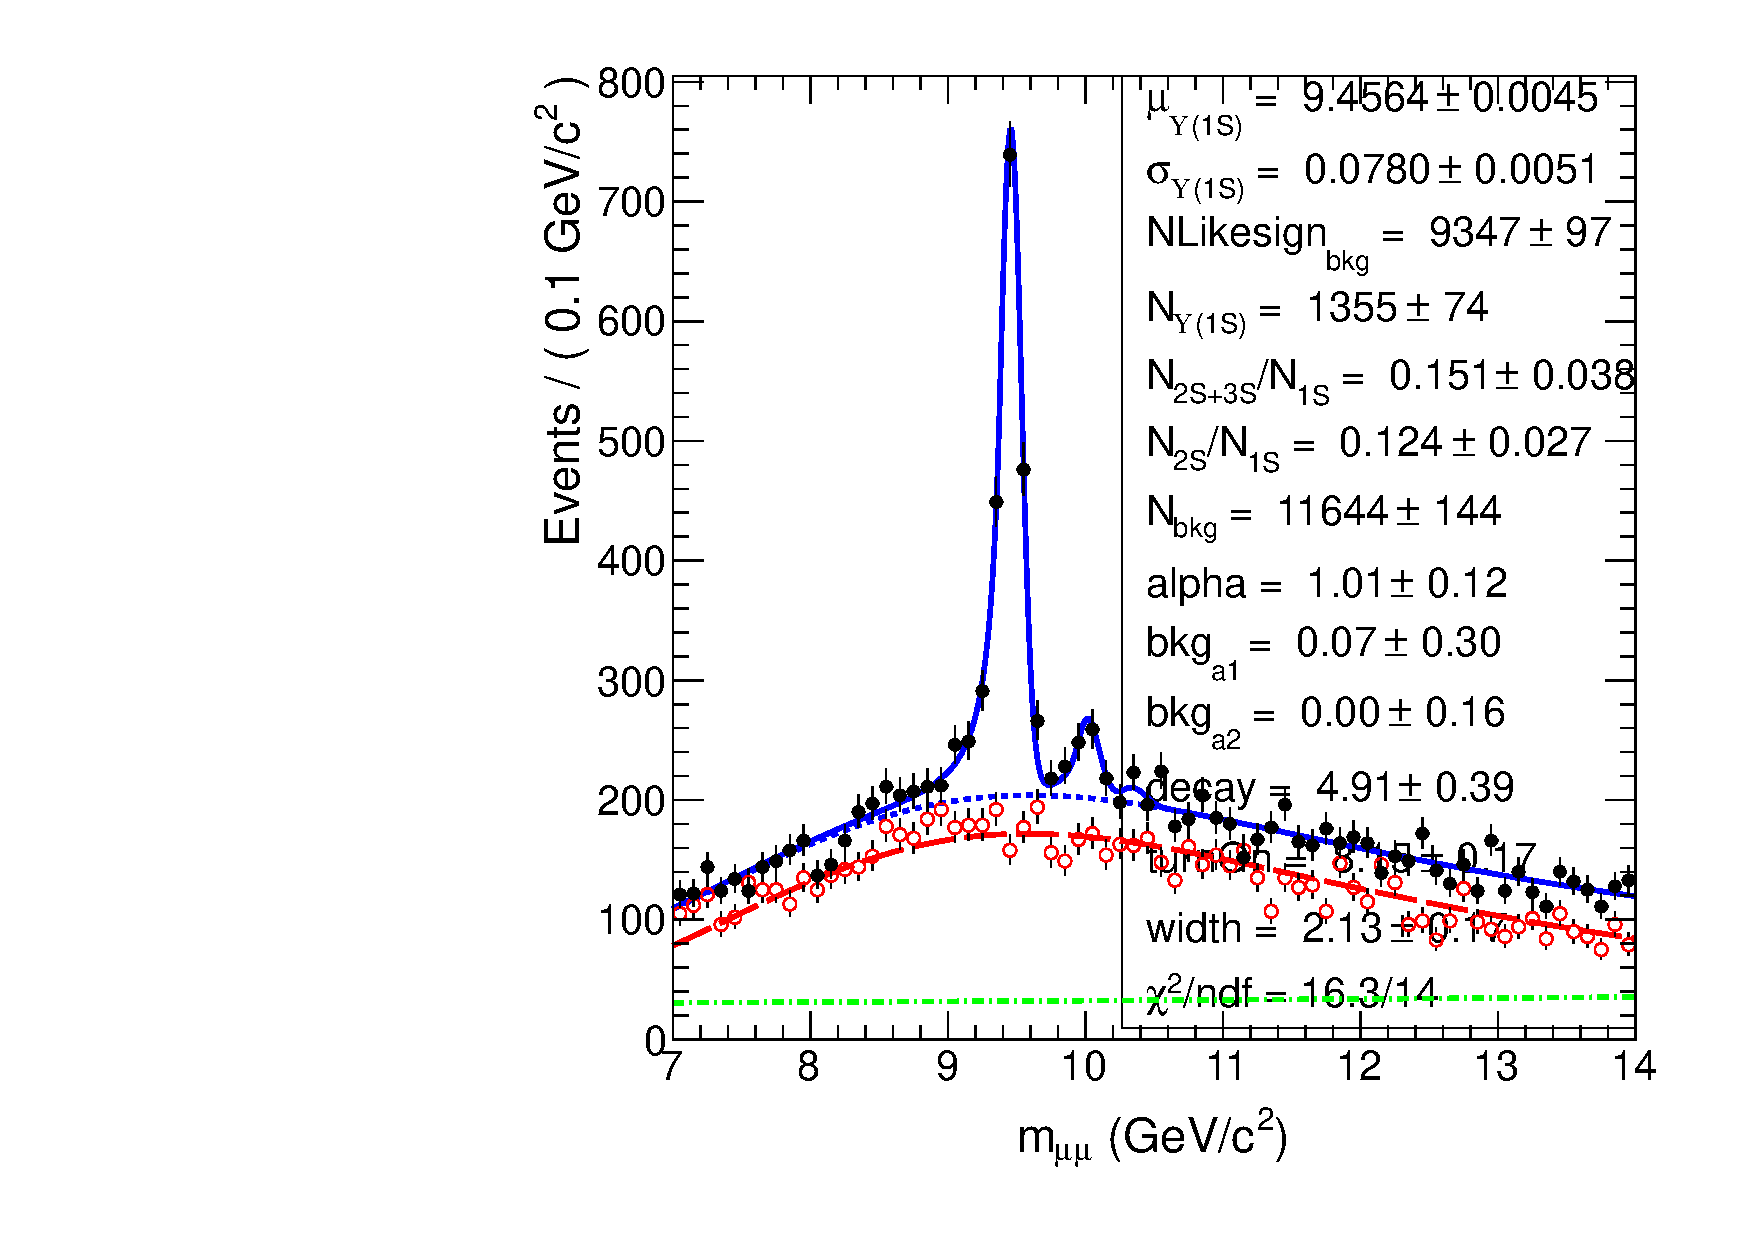
\includegraphics[angle=0,width=0.3\textwidth]{figures/fulldataset/masspeak_hi_LSerf.pdf}\label{fig:final_PbPb_LSerf}}
    \subfigure[LS TrkRot erf*exp + pol2]{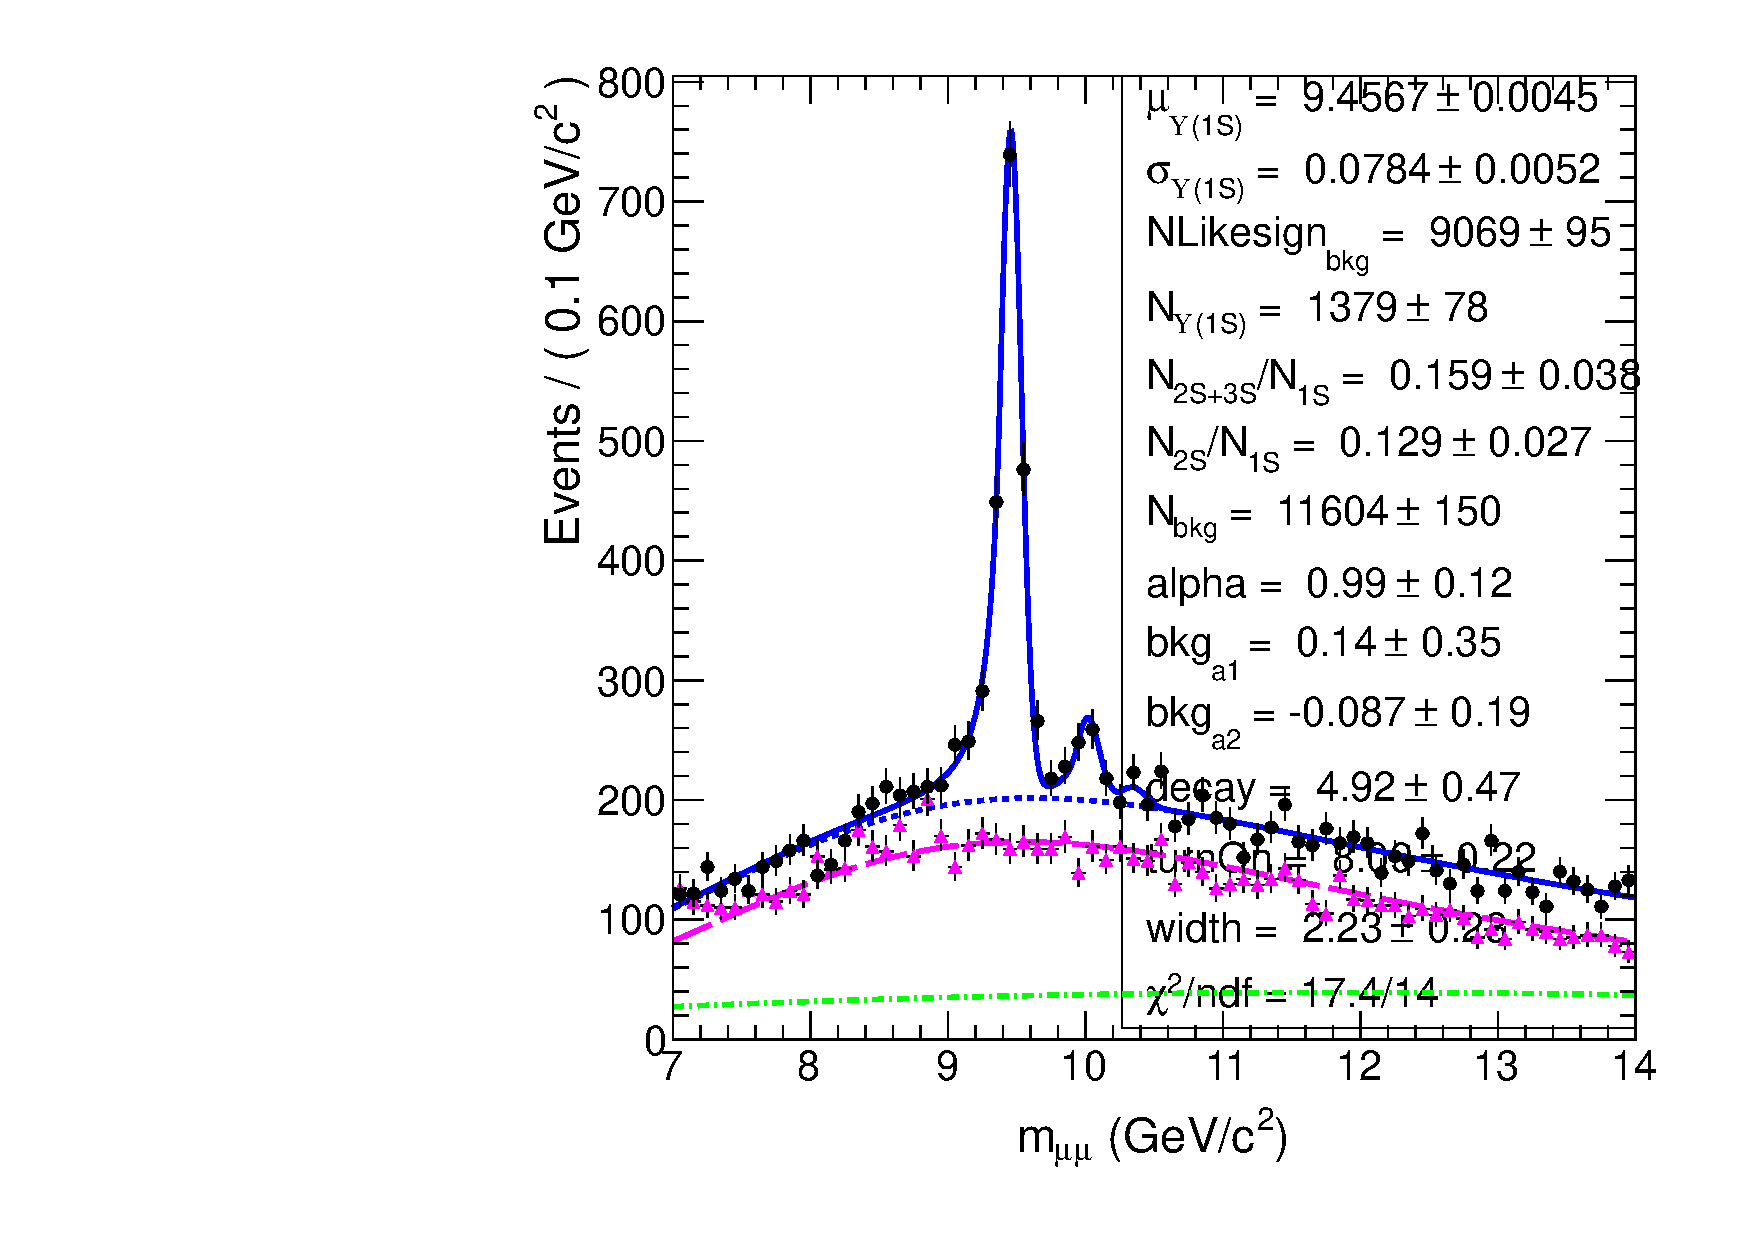
\includegraphics[angle=0,width=0.3\textwidth]{figures/fulldataset/masspeak_hi_TRerf.pdf}\label{fig:final_PbPb_TRerf}}
    \subfigure[OS TrkRot erf*exp + pol2]{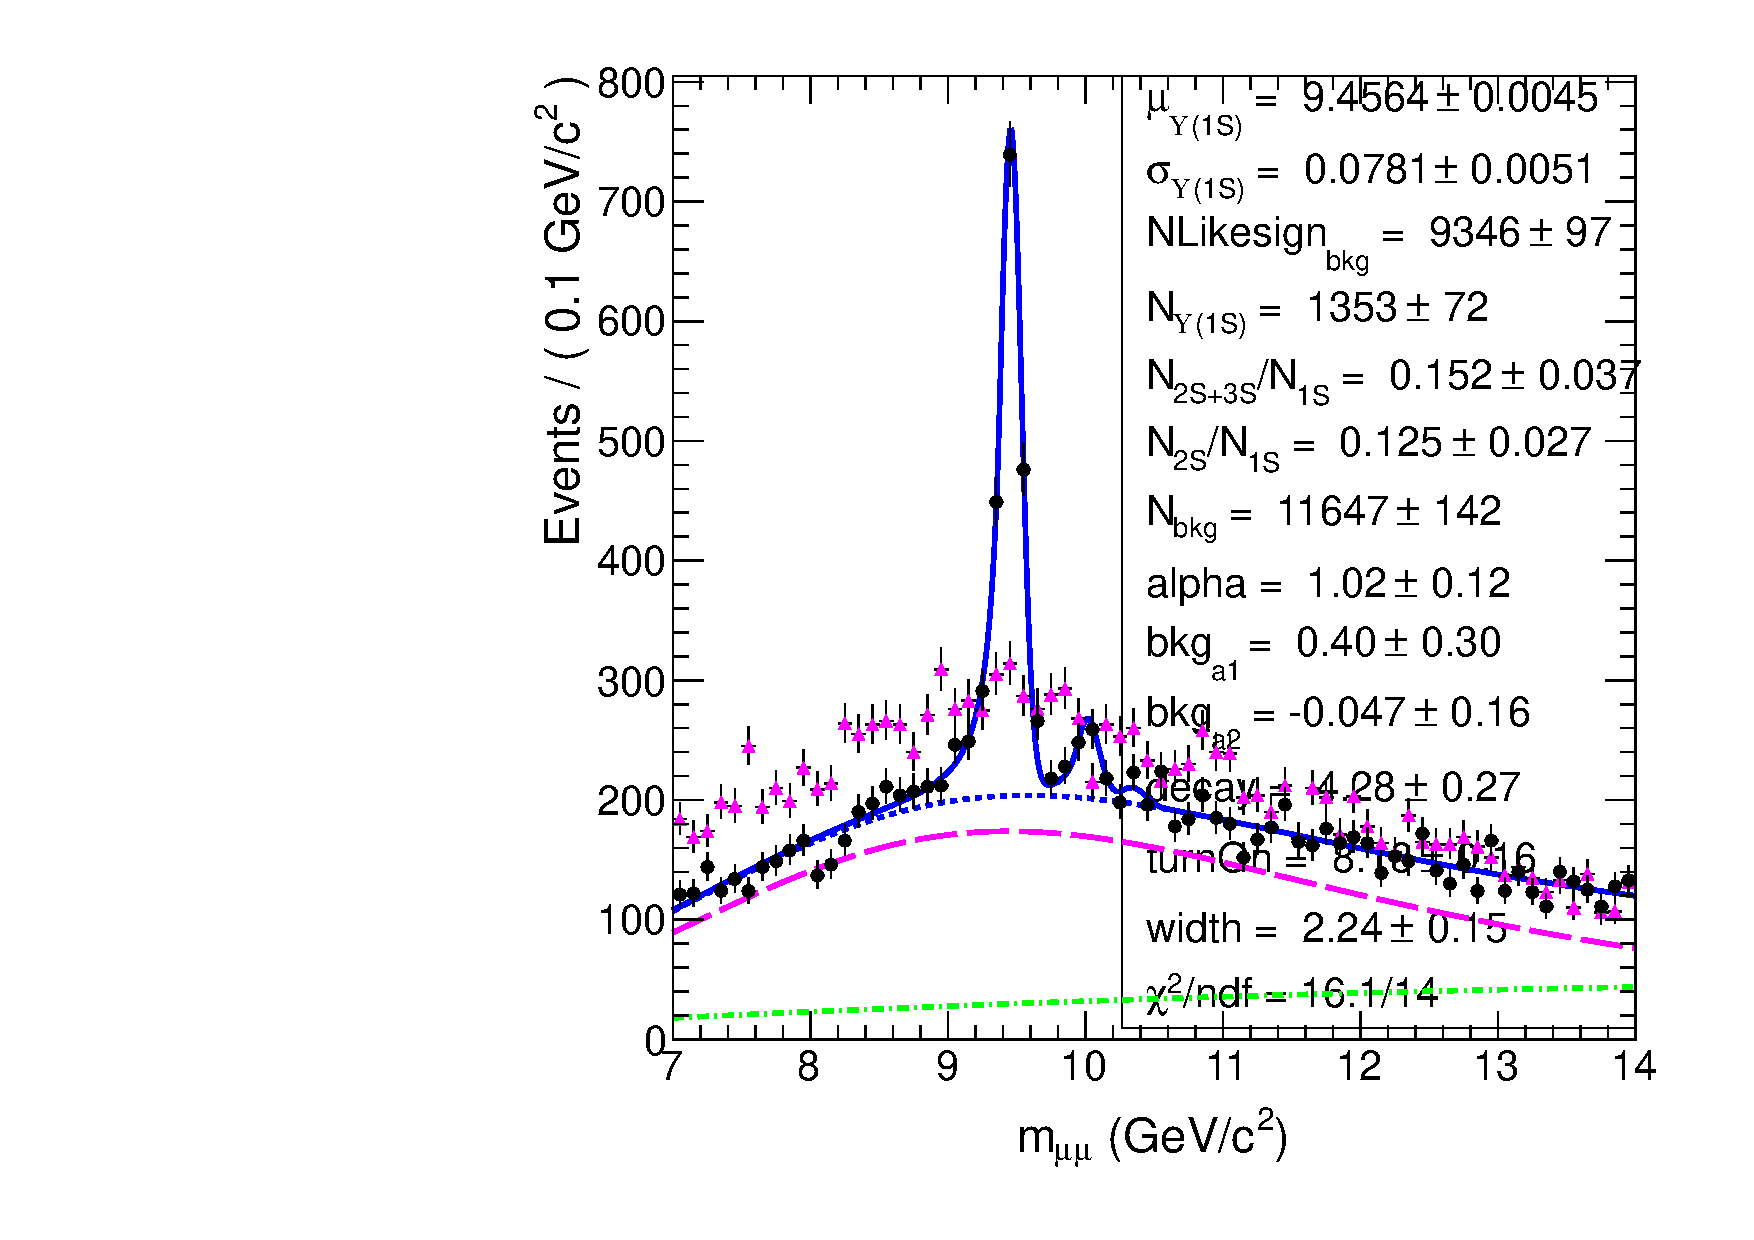
\includegraphics[angle=0,width=0.3\textwidth]{figures/fulldataset/masspeak_Hi_paramOn_OS_trkRot.pdf}\label{fig:final_PbPb_TRerf_OS}}
  \caption{PbPb fit model variations ($150 \mu b^{-1}$).}
  \label{fig:PbPb_model_variations}
  \end{center}
\end{figure}

The associated systematic uncertainties are summarized in Table~\ref{tab:final-single-rat} for \PbPb, and in Table~\ref{tab:final-single-rat-pp} for \pp.  
%
From the several variations, two estimates of the systematic uncertainty are provided: 
(i) the quadratic-mean deviation relative to the nominal central value, RMS (schematically, $\sqrt{(\sum{\text{variation - nominal})^2} / (n-1)}$); and (ii) the largest deviation. 
The latter is used as the estimated systematic uncertainty.

\begin{table}[!h]
  \centering
  \caption{Summary of single-ratio results, for the PbPb dataset.}
  \begin{tabular}{l|c|c|c}
    \hline
 &\multicolumn{3}{|c}{$\pt^\mu>4\GeVc$, Cent. 0-100\%}\\
 &\multicolumn{1}{|c}{$R_{23}$}& \multicolumn{1}{|c}{$R_{2}$} & \multicolumn{1}{|c}{$R_{3}$} \\
\hline
nominal (erf*exp)                   & $0.155\pm 0.038$ & $0.127\pm 0.027$ & $0.027\pm0.025$ \\
\hline
 \multicolumn{4}{l}{systematic variations:} \\
like-sign (LS) keyspdf + pol.2      & $0.159\pm 0.037$ & $0.130\pm 0.027$ &  $0.029\pm0.046 $  \\
LS erf*exp + pol.2                  & $0.151\pm 0.038$ & $0.124\pm 0.027$ &  $0.027\pm0.047 $   \\
%LS Track Rotation (TR) keyspdf + pol.2 & $0.170\pm 0.036$ & $0.137\pm 0.026$ &  $0.033\pm0.044 $  \\
%LS TR erf*exp + pol.2               & $0.159\pm 0.038$ & $0.129\pm 0.027$ &  $0.030\pm0.047 $   \\  
opposite-sign (OS) Track Rotation (TR) keyspdf + pol.2 & $0.157\pm 0.037$ & $0.120\pm 0.027$ &  $0.037\pm0.046 $  \\
OS TR erf*exp + pol.2               & $0.152\pm 0.037$ & $0.125\pm 0.027$ &  $0.025\pm0.046 $   \\
fix CB tail from MC (alpha = 1.4)   & $0.130\pm 0.038$ & $0.113\pm 0.027$ &  $0.017\pm0.047 $   \\
fix resolution from MC (92 \MeVcc)  & $0.159\pm 0.038$ & $0.128\pm 0.028$ &  $0.031\pm0.047 $  \\
fix both CB and resolution from MC  & $0.140\pm 0.037$ & $0.118\pm 0.027$ &  $0.022\pm0.046 $  \\
\hline
fit systematic (RMS)              & 0.011 & 0.007 & 0.005  \\
fit systematic (largest variation)& 0.026 & 0.016 & 0.015  \\
\hline
 \multicolumn{4}{l}{other checks:} \\
%opposite-sign (OS) TR keyspdf + pol.2 & $0.157\pm 0.037$ & $0.120\pm 0.027$ &  $0.037\pm0.046 $  \\ 
%OS TR erf*exp + pol.2               & $0.152\pm 0.037$ & $0.125\pm 0.027$ &  $0.025\pm0.046 $   \\ 
LS Track Rotation (TR) keyspdf + pol.2 & $0.170\pm 0.036$ & $0.137\pm 0.026$ &  $0.033\pm0.044 $  \\
LS TR erf*exp + pol.2               & $0.159\pm 0.038$ & $0.129\pm 0.027$ &  $0.030\pm0.047 $   \\
\hline
nominal simultaneous fit (erf*exp)  & $0.143\pm 0.038$ & $0.119\pm 0.027$ & $0.024\pm0.024$ \\
\hline
%efficiency systematic             & 4.6\% & 4.6\% & 4.6\%  \\
%\hline
%total systematic                  & 0.015 & 0.010 & 0.005 \\
%\hline
  \end{tabular}
  \label{tab:final-single-rat}
\end{table}

\begin{table}[!h]
  \centering
  \caption{Summary of single-ratio results for the \Pp\Pp{} 2.76 TeV dataset.}
  \begin{tabular}{l|c|c|c}
    \hline
 &\multicolumn{3}{|c}{$\pt^\mu>4\GeVc$}\\ 
 &\multicolumn{1}{|c}{$R_{23}$}& \multicolumn{1}{|c}{$R_{2}$} & \multicolumn{1}{|c}{$R_{3}$} \\  
\hline
nominal (pol2; signal pdf fixed from PbPb)    & $0.88\pm 0.17$ & $0.50\pm 0.12$ & $0.38\pm 0.10$ \\
\hline
 \multicolumn{4}{l}{systematic variations:} \\
fix CB tail from MC                      & $0.85\pm 0.16$ & $0.49\pm 0.11$ & $0.36\pm0.19 $  \\
fix resolution from MC                   & $0.89\pm 0.16$ & $0.49\pm 0.12$ & $0.40\pm0.20 $  \\
fix both CB and resolution               & $0.87\pm 0.16$ & $0.49\pm 0.11$ & $0.38\pm0.19 $  \\
erf*exp                                  & $0.86\pm 0.16$ & $0.49\pm 0.11$ & $0.37\pm0.19 $   \\  
LS keyspdf + pol.2                       & $0.84\pm 0.17$ & $0.48\pm 0.12$ & $0.36\pm0.21 $   \\  
LS erf*exp + pol.2                       & $0.87\pm 0.16$ & $0.49\pm 0.12$ & $0.38\pm0.20 $   \\  
\hline
fit systematic (RMS)               & 0.023 & 0.012 & 0.015  \\  
fit systematic (largest variation) & 0.051 & 0.024 & 0.035  \\
\hline
nominal simultaneous fit (pol2)  & $0.97\pm 0.19$ & $0.56\pm 0.13$ & $0.41\pm0.11$ \\
\hline
%efficiency systematic              & 6.2\% & 6.2\% & 6.2\%  \\
%\hline
%total systematic                   & 0.059 & 0.033 & 0.028  \\
%\hline
  \end{tabular}
  \label{tab:final-single-rat-pp}
\end{table}


\subsection{Centrality dependence}

Effects induced by the hot medium are expected to display, in general, a dependence on the centrality of the collision -- the effect is more accentuated for the most central collision events, and approaching the most peripheral events tend asymptotically towards the results expected in the absence of medium effects. 
%The pp collision results are usually %is sometimes
% taken as reference for the un-modified case. 
%Such basic behaviour can nonetheless be challenged, as a consequence of complexity of the underlying phenomena.  
%
The \pp collision results are taken as reference for absence of nuclear effects. 
%for the un-modified case. 

We repeat the single ratio measurement, by splitting the PbPb dataset in ranges of the collision centrality. 
The mass fit results are shown in Figures~\ref{fig:final_massfit_singlerat_centrality}.

The systematic uncertainties are evaluated for the nominal selection, and summarized in Table~\ref{tab:final_singlerat_centrality}. The corresponding differential results are displayed in \fig{fig:final_singlerat_centrality_nominal}. In these plots, the single ratio values are normalized by the central value of the measurement performed using the \Pp\Pp{} data. Note these normalization values depend on the \pt{} threshold case, and are obtained from the fit to the \Pp\Pp{} data with constrained signal shape from MC, displayed in Table~\ref{tab:final-single-rat-pp}. 
 Uncertainties on the single-point \Pp\Pp~measurement are not included, as such common uncertainty factor is not relevant for point-to-point comparison in this plot showing the double ratio trend with $N_{part}$. Some error bars in \fig{fig:final_singlerat_centrality_nominal} reach negative values, so we refine this using Feldman-Cousins limit calculation as shown in \fig{fig:final_singlerat_centrality_limit}. 

 
\begin{figure}[hbtp]
  \begin{center}
\subfigure[ 0-  5\%]{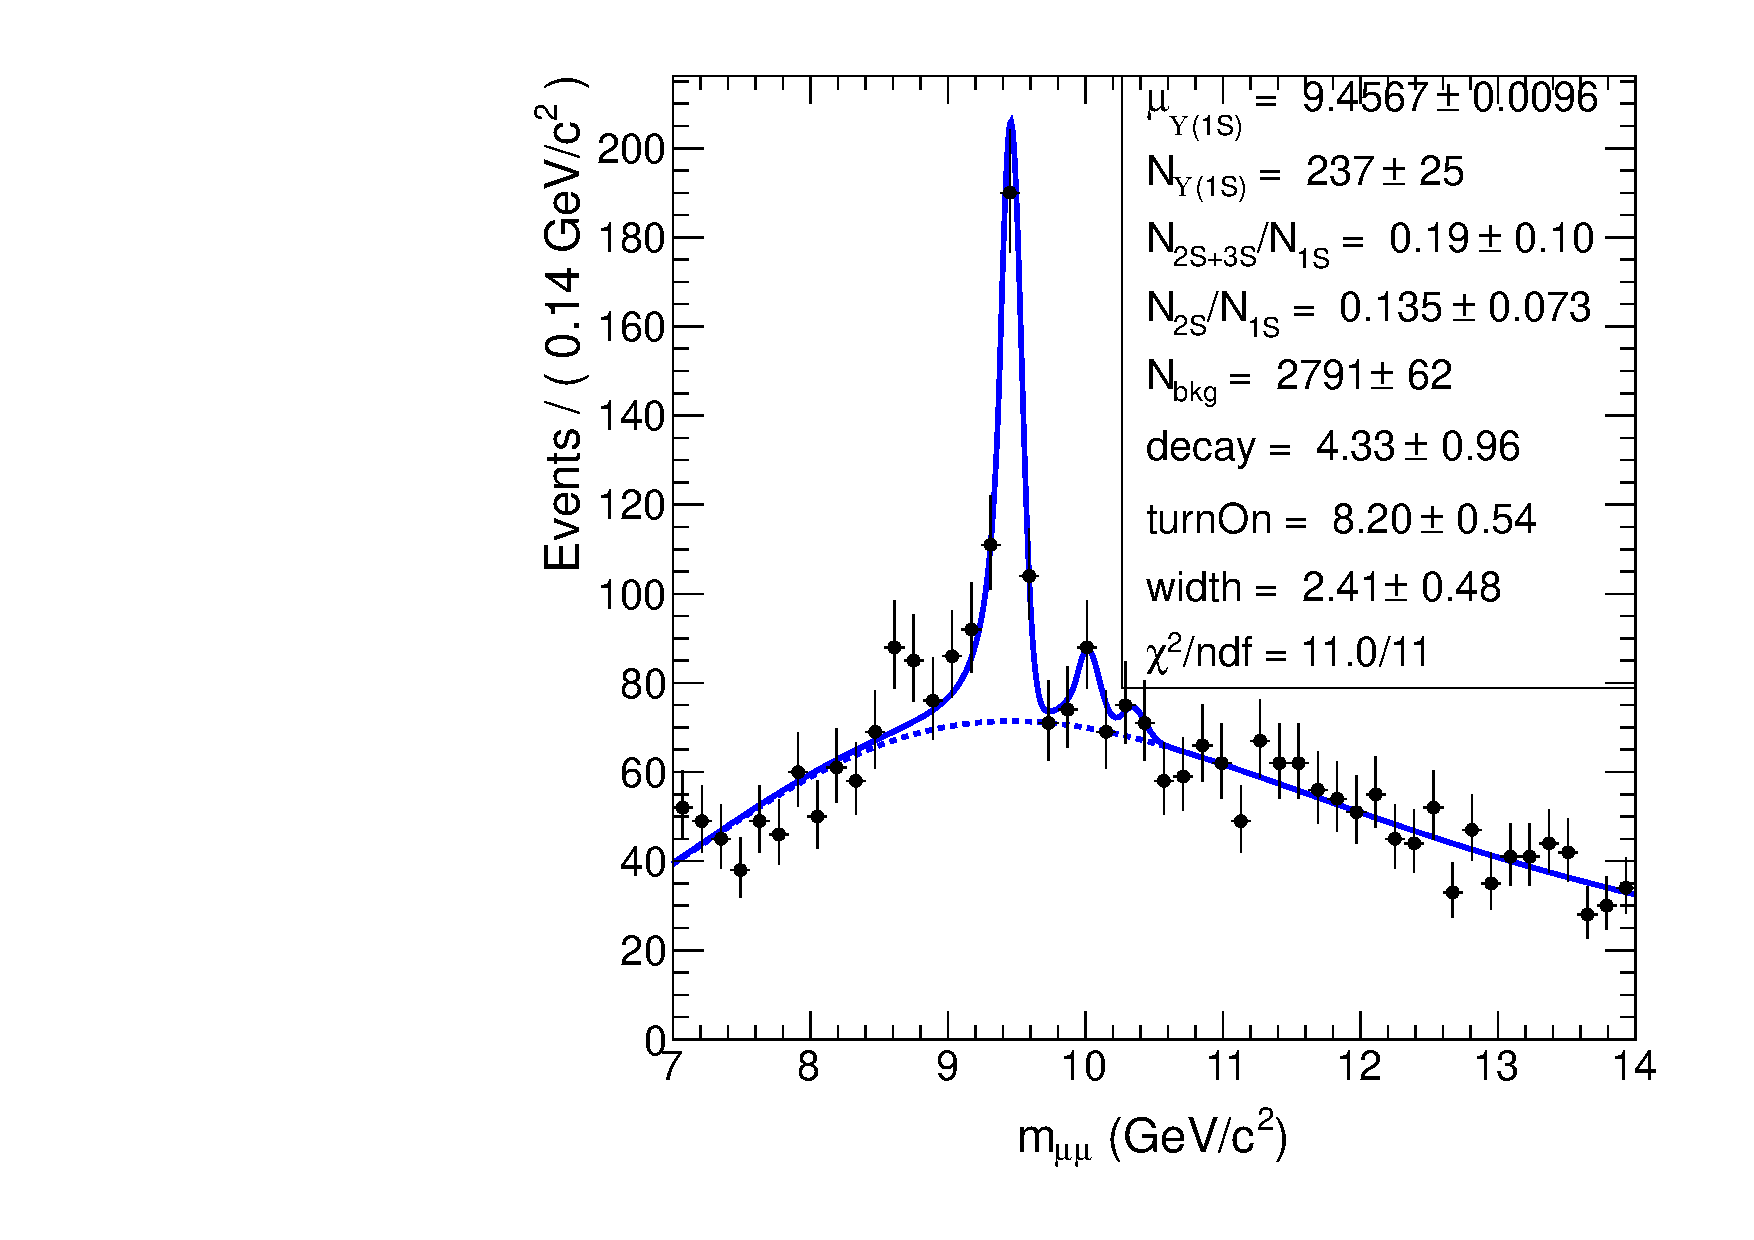
\includegraphics[angle=0,width=0.3\textwidth]{figures/fulldataset/masspeak_Hi_paramOn_cntr0-5}}
\subfigure[ 5- 10\%]{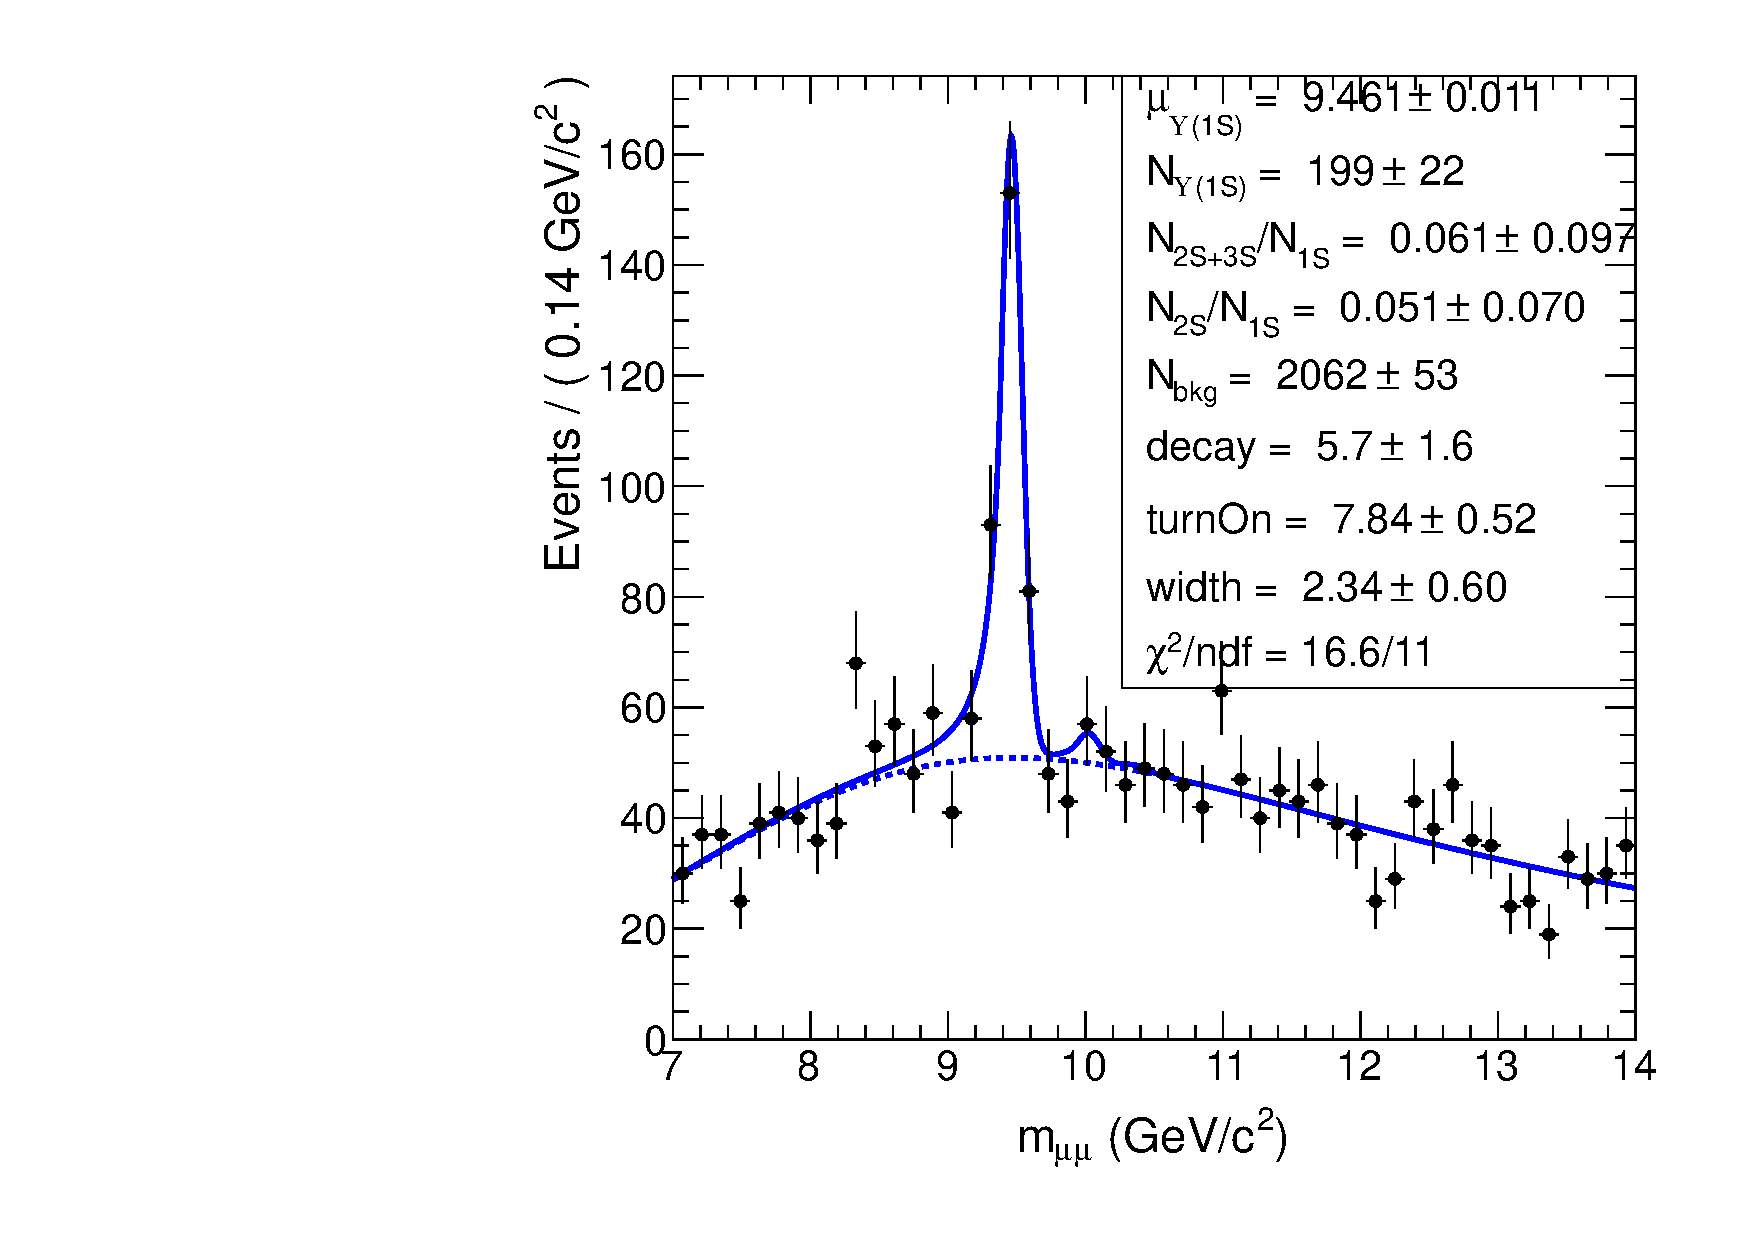
\includegraphics[angle=0,width=0.3\textwidth]{figures/fulldataset/masspeak_Hi_paramOn_cntr5-10}}
\subfigure[10- 20\%]{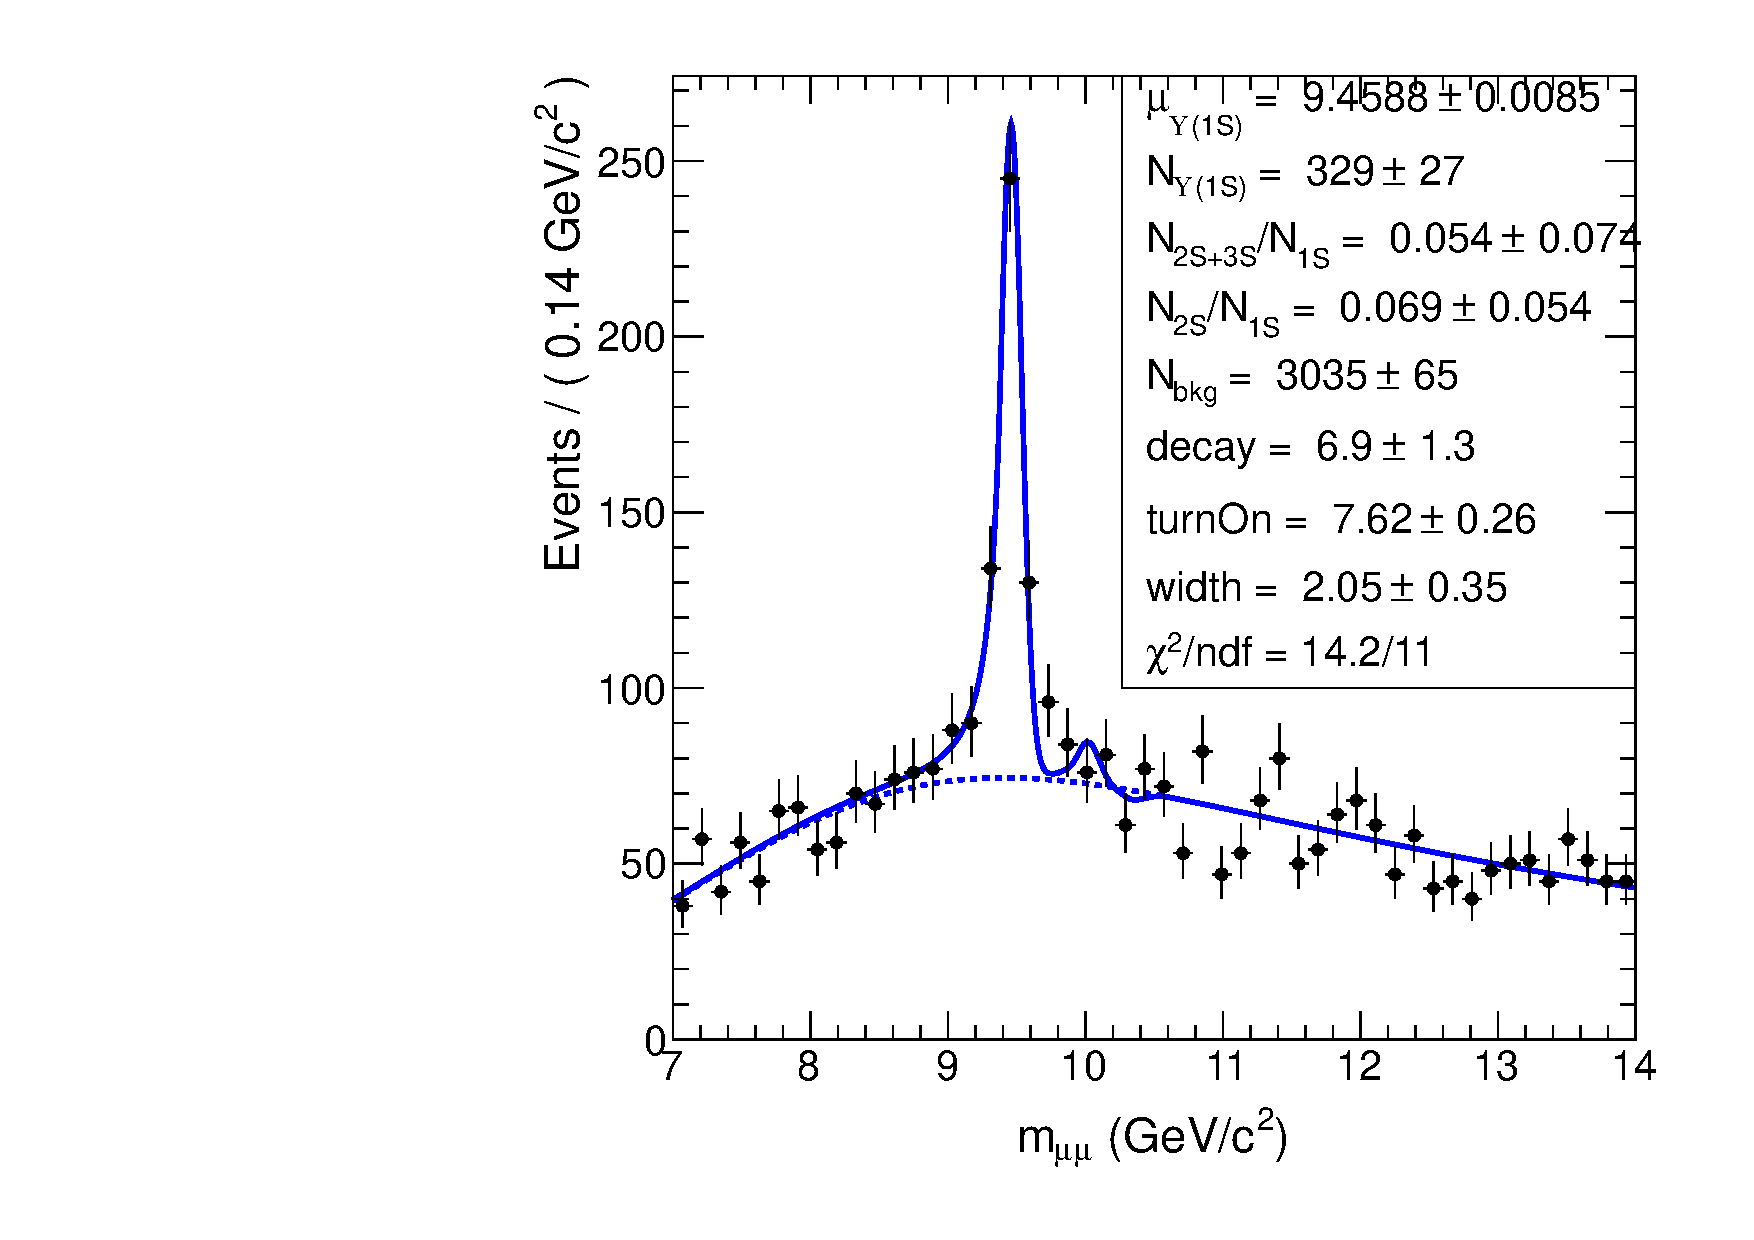
\includegraphics[angle=0,width=0.3\textwidth]{figures/fulldataset/masspeak_Hi_paramOn_cntr10-20}}\\
\subfigure[20- 30\%]{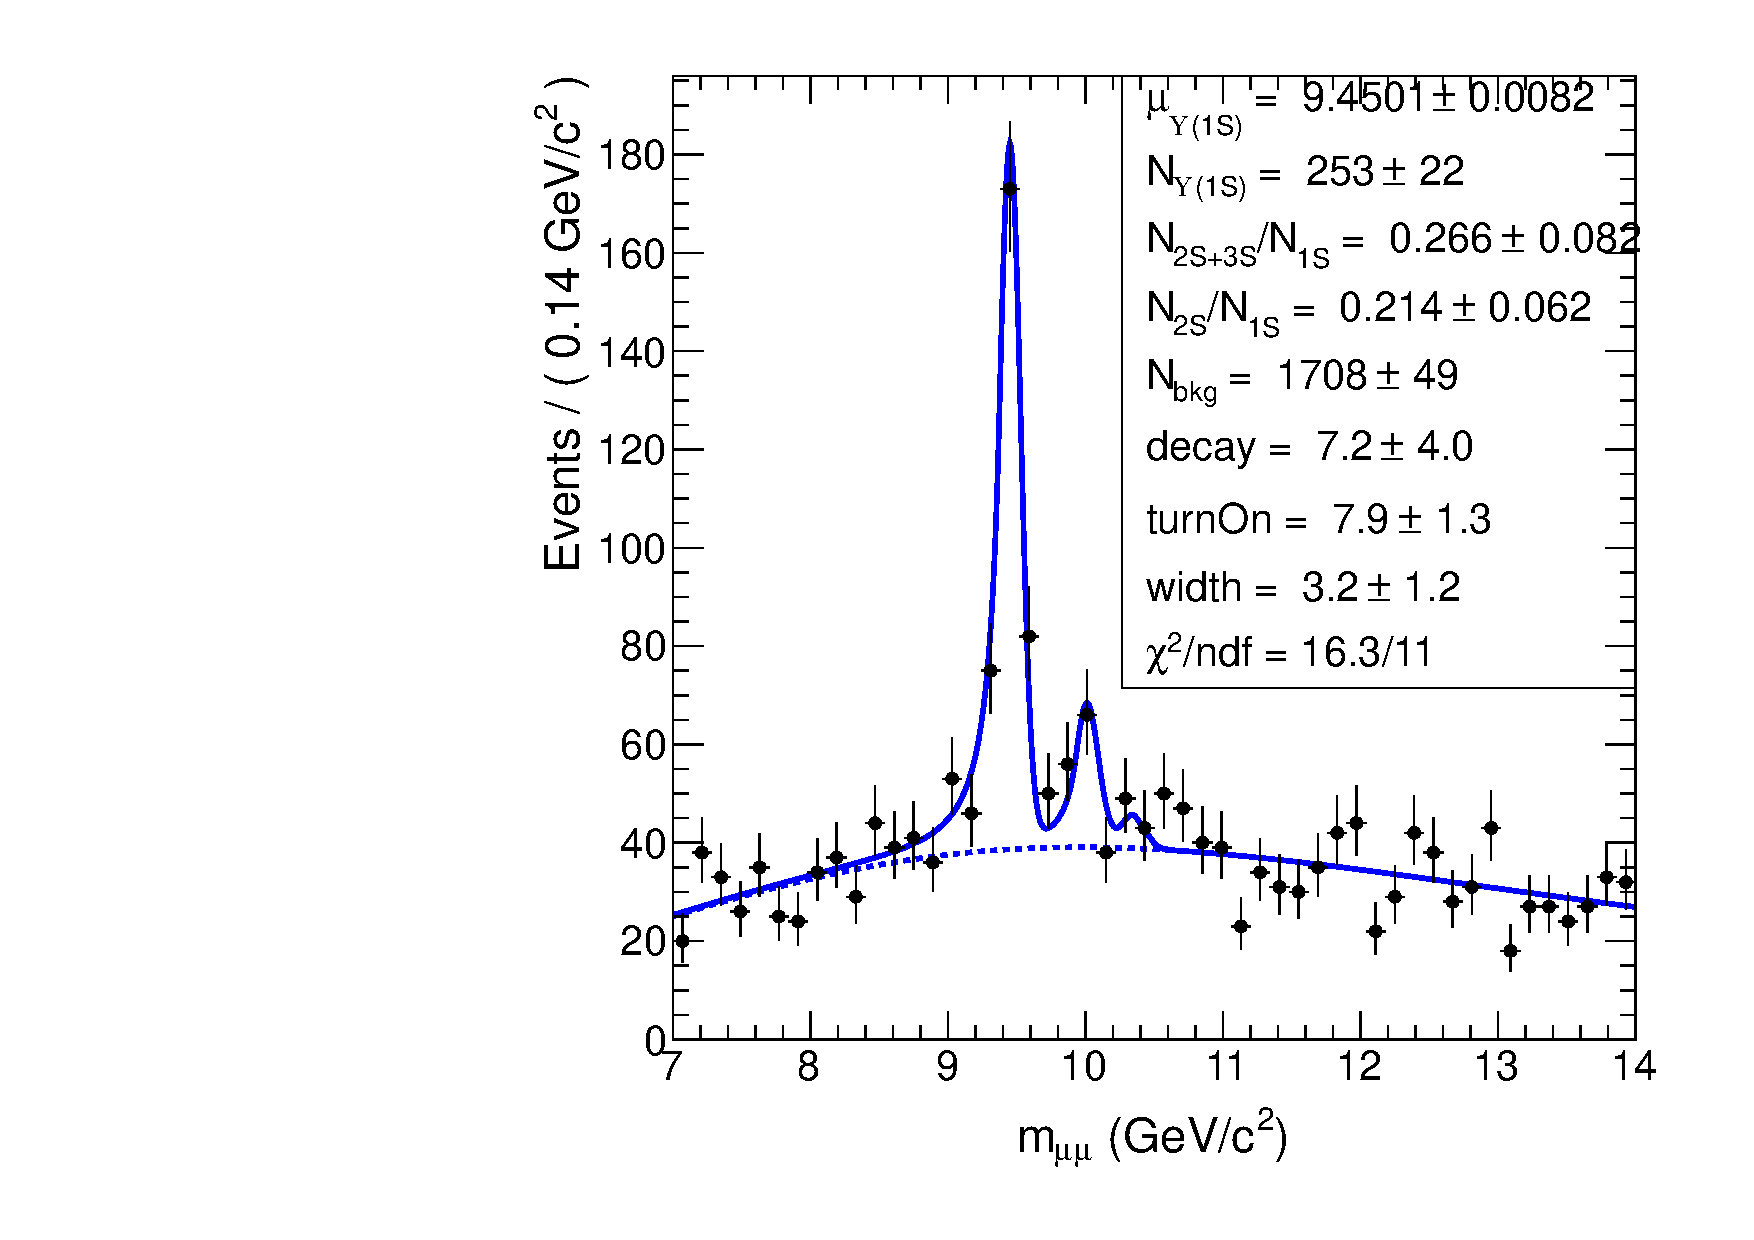
\includegraphics[angle=0,width=0.3\textwidth]{figures/fulldataset/masspeak_Hi_paramOn_cntr20-30}}
\subfigure[30- 40\%]{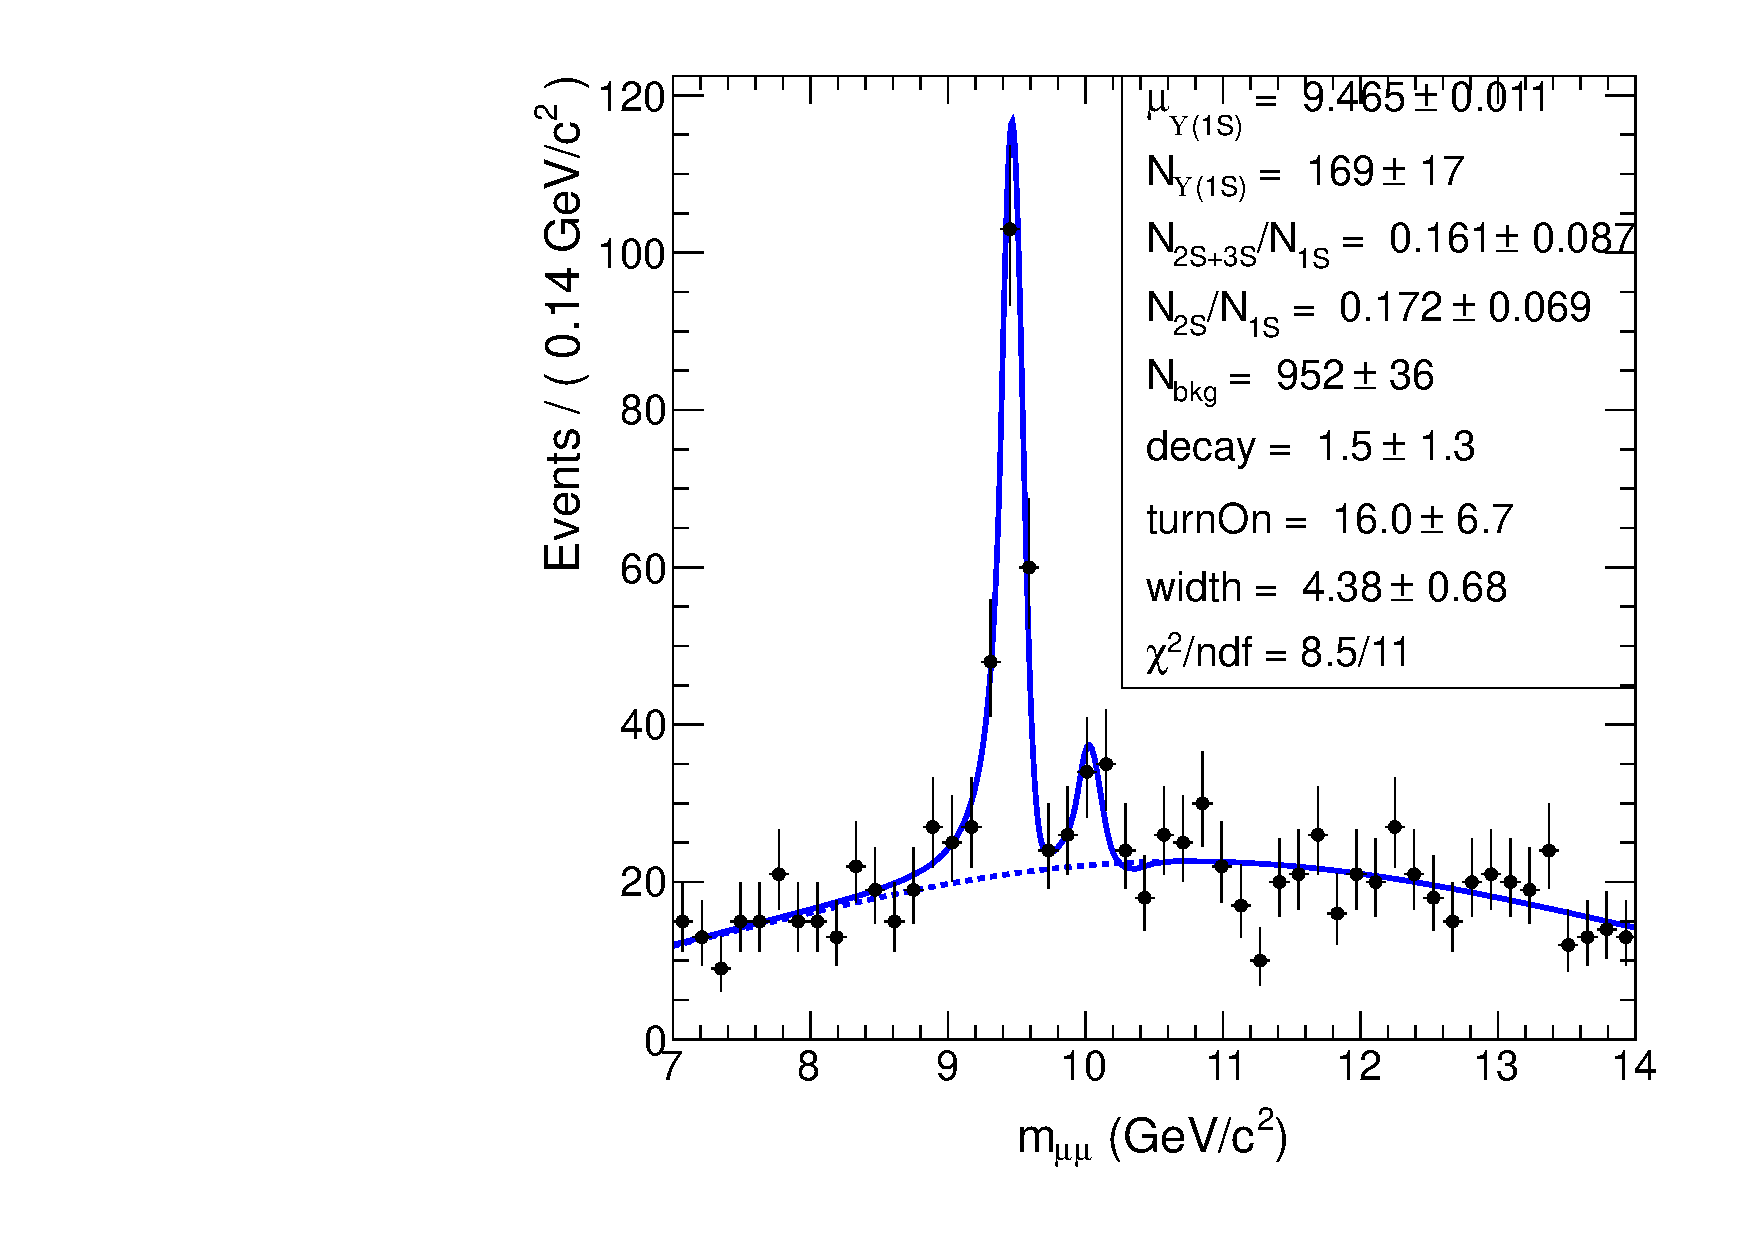
\includegraphics[angle=0,width=0.3\textwidth]{figures/fulldataset/masspeak_Hi_paramOn_cntr30-40}}
\subfigure[40- 50\%]{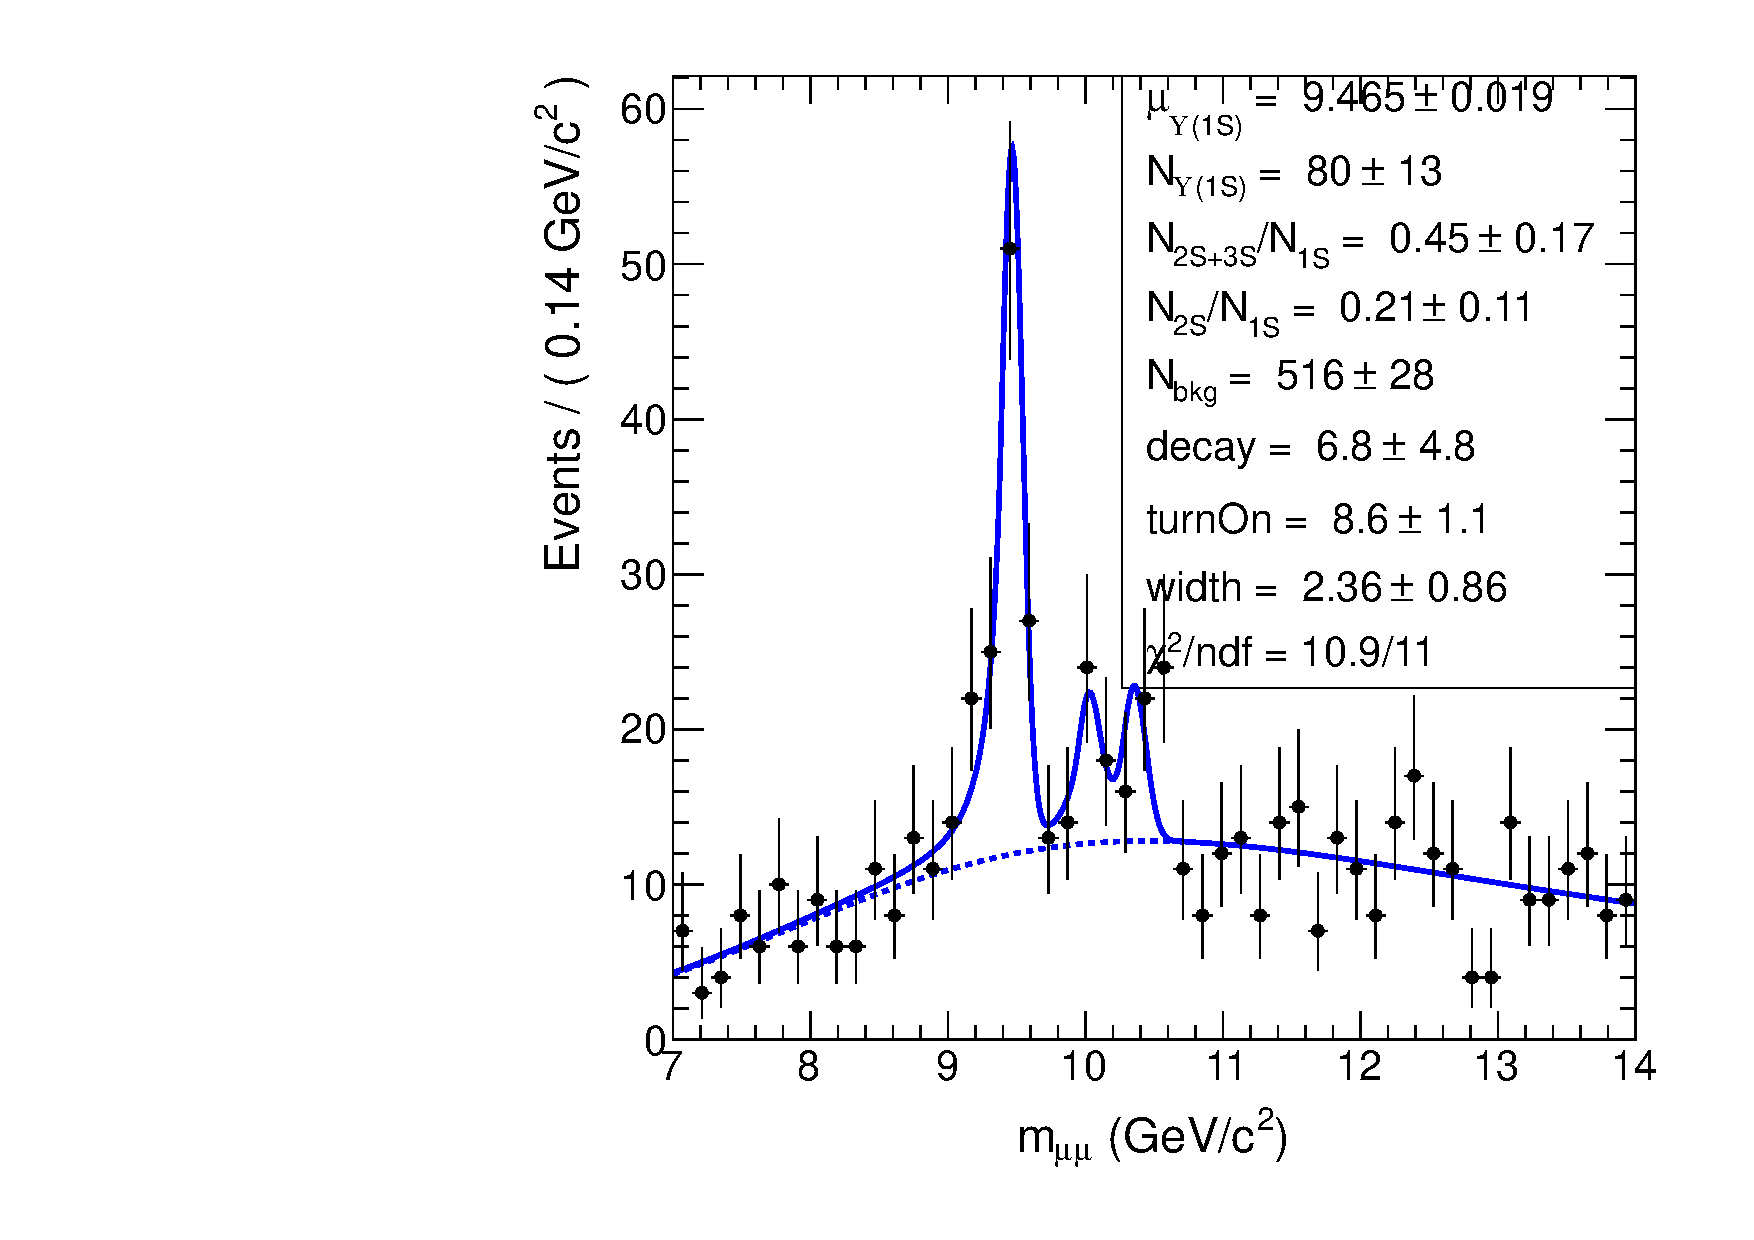
\includegraphics[angle=0,width=0.3\textwidth]{figures/fulldataset/masspeak_Hi_paramOn_cntr40-50}}\\
\subfigure[50-100\%]{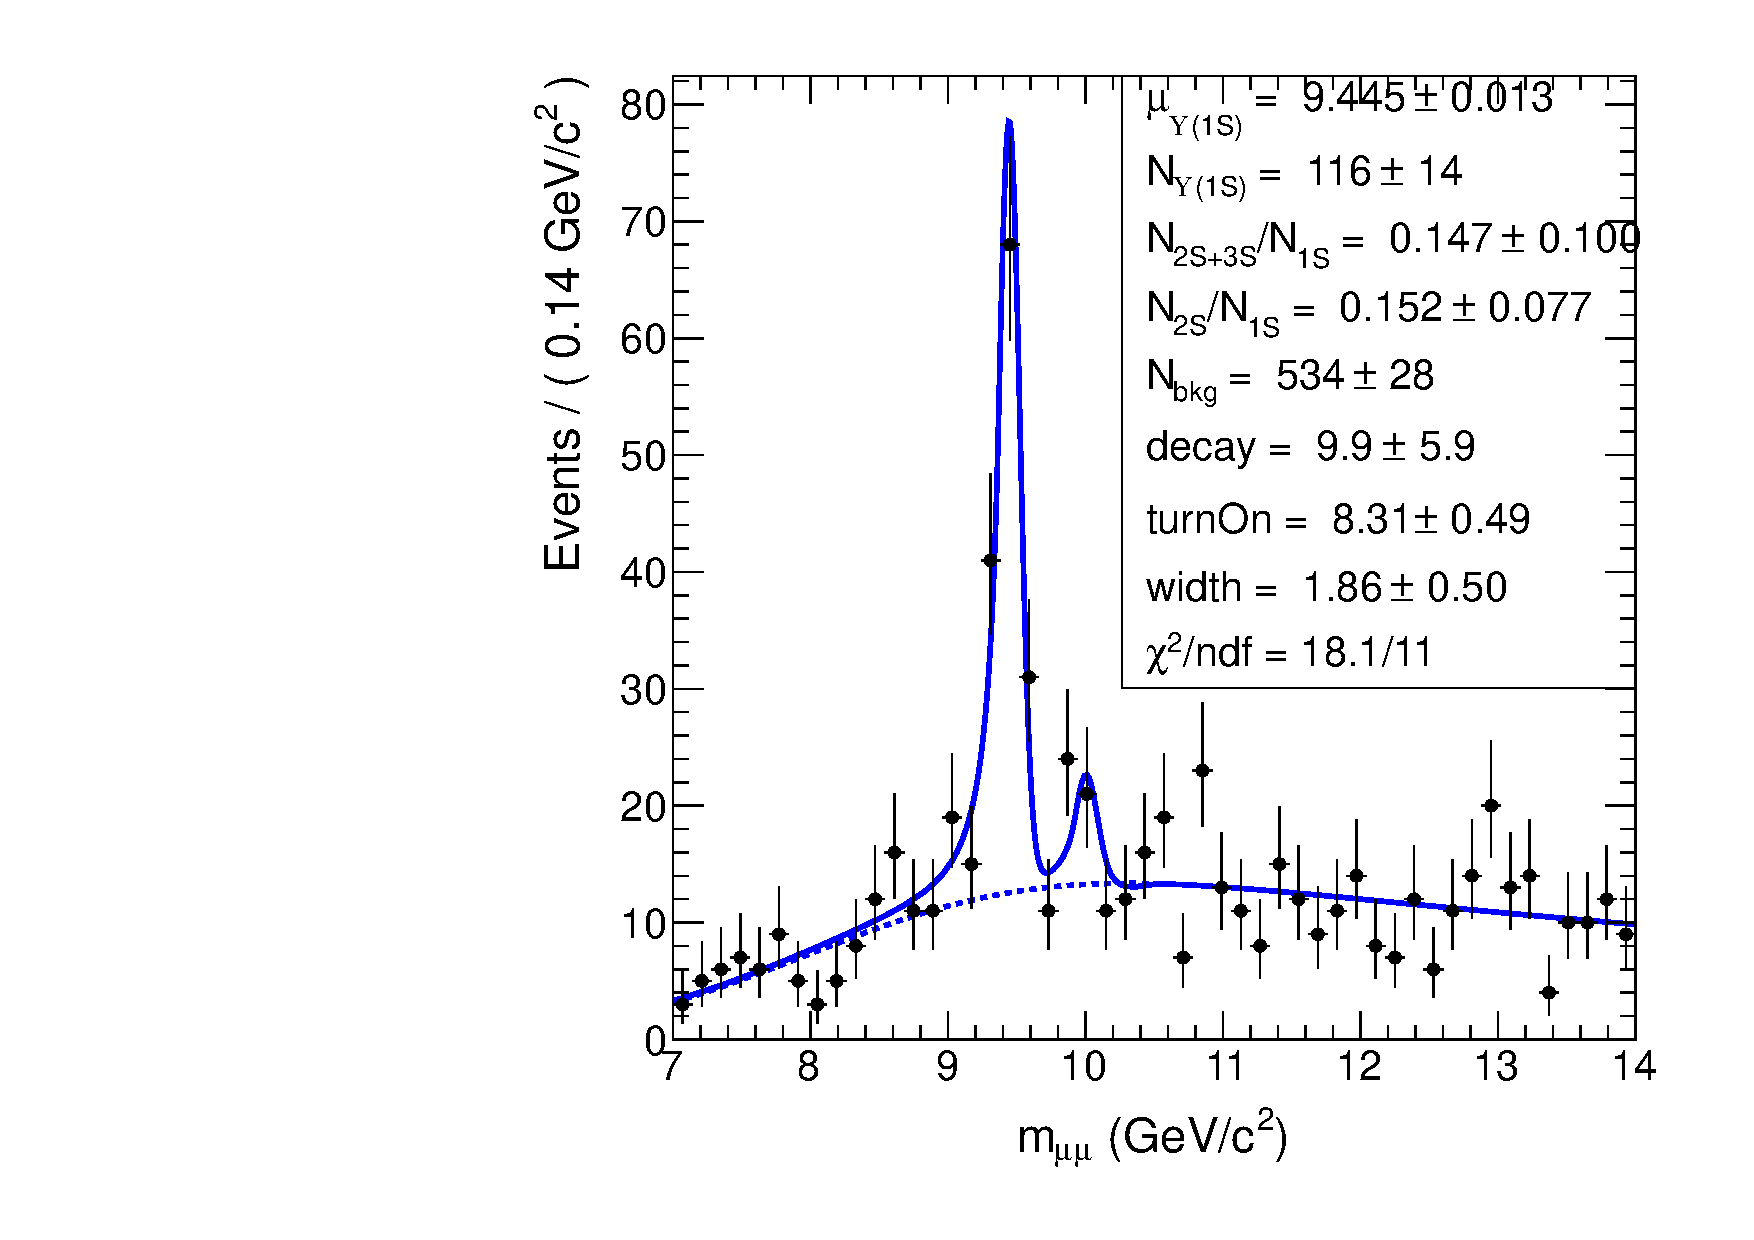
\includegraphics[angle=0,width=0.3\textwidth]{figures/fulldataset/masspeak_Hi_paramOn_cntr50-100}}
\subfigure[50- 60\%]{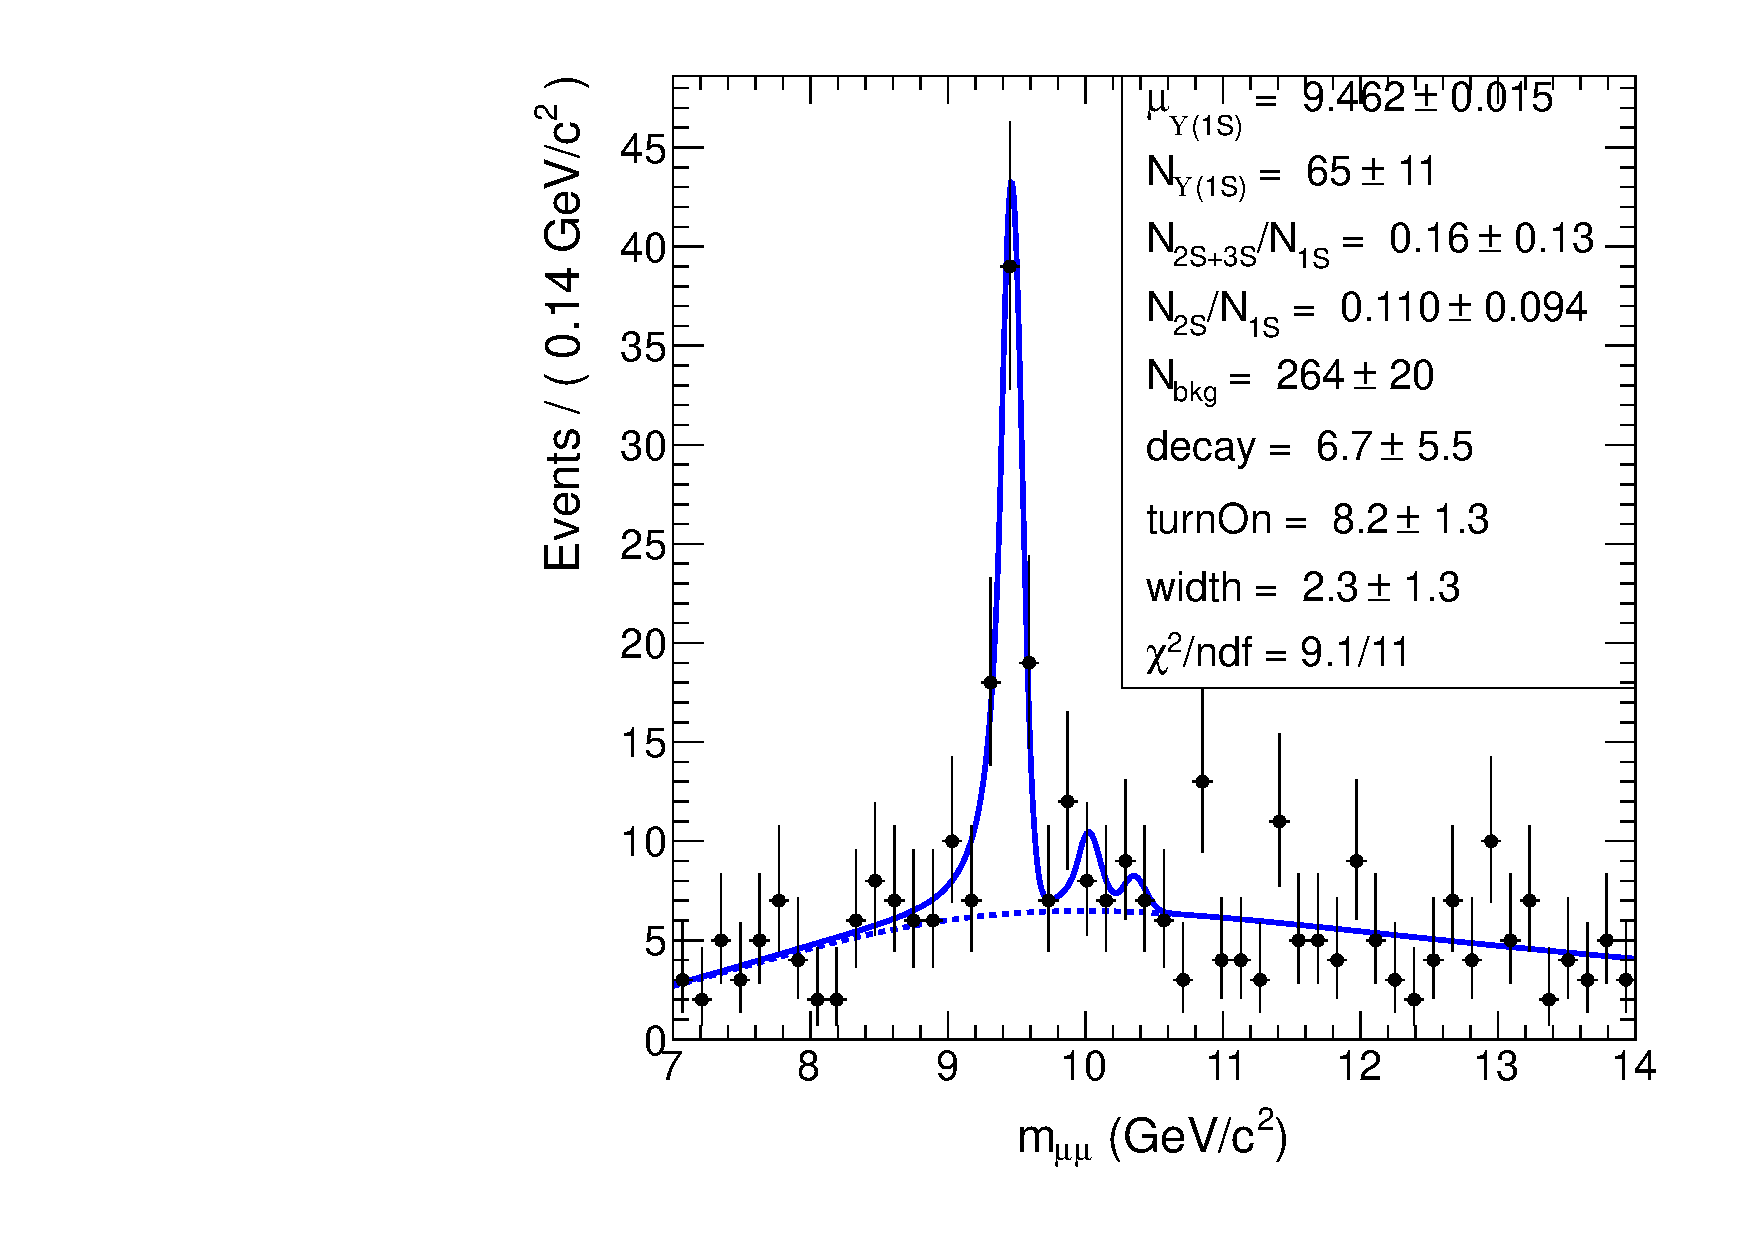
\includegraphics[angle=0,width=0.3\textwidth]{figures/fulldataset/masspeak_Hi_paramOn_cntr50-60}}
\subfigure[60-100\%]{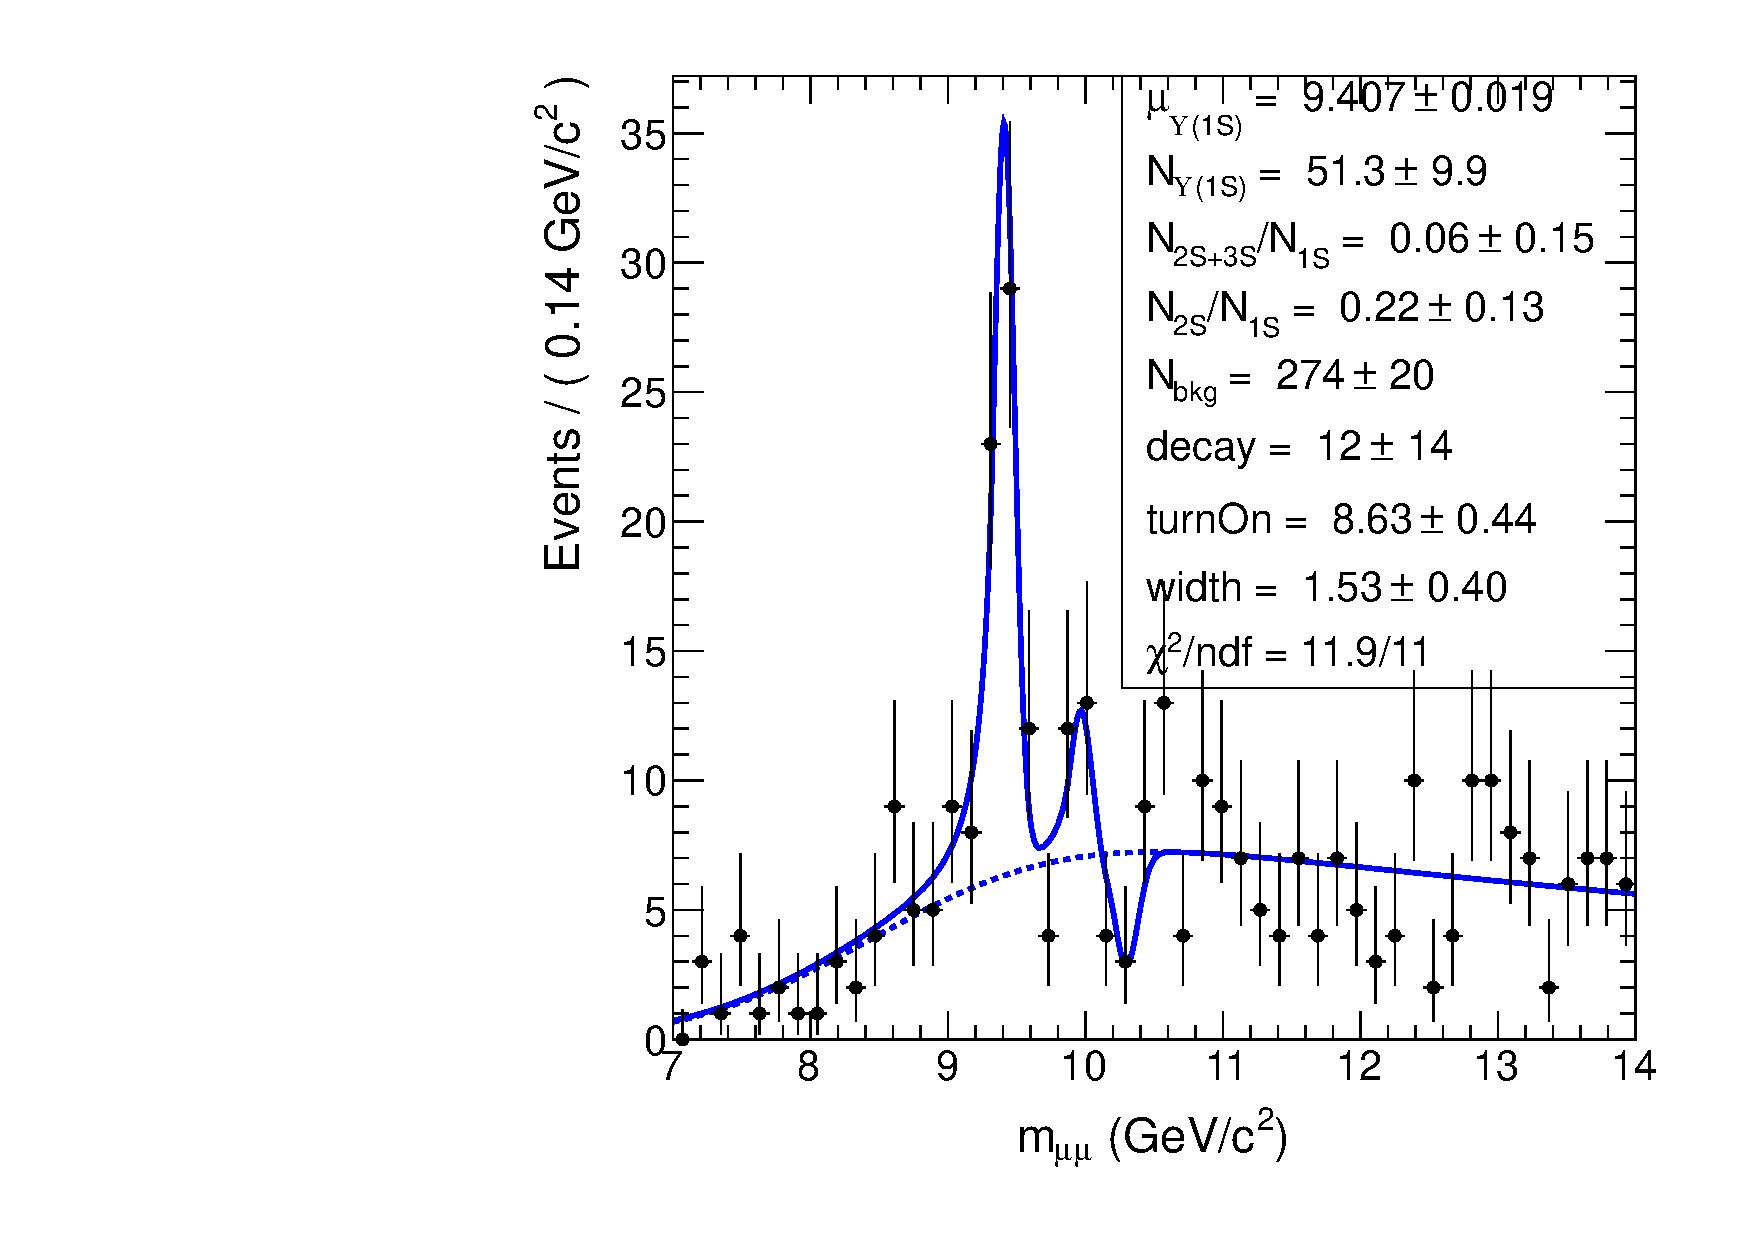
\includegraphics[angle=0,width=0.3\textwidth]{figures/fulldataset/masspeak_Hi_paramOn_cntr60-100}}
\caption{Centrality dependence of the PbPb single ratio, for $\pt^\mu>4.0\GeVc$. ($150 \mu b^{-1}$).}
  \label{fig:final_massfit_singlerat_centrality}
  \end{center}
\end{figure}


\begin{sidewaystable}[!h]
  \centering
  \caption{Summary of single-ratio centrality dependent results.
}
  \begin{tabular}{c|ccccccc}
    \hline
 &  0-5\% & 5-10\% & 10-20\% & 20-30\% & 30-40\% & 40-50\% & 50-100\% \\
\hline

\hline
 \multicolumn{8}{l}{$R_{23} \quad (\pt^\mu>4.0\GeVc)$} \\
nominal result             & $0.190\pm0.100$ & $0.061\pm0.097$ & $0.054\pm0.074$ & $0.266\pm0.082$ & $0.161\pm0.087$ & $0.450\pm0.170$ & $0.147\pm0.100$ \\
\hline
 \multicolumn{8}{l}{systematic variations:} \\
LS keyspdf + pol.2         & $0.220\pm0.099$ & $0.009\pm0.097$ & $0.030\pm0.075$ & $0.246\pm0.079$ & $0.125\pm0.088$ & $0.488\pm0.160$ & $0.165\pm0.095$ \\
TR keyspdf + pol.2         & $0.237\pm0.097$ &$-0.011\pm0.093$ & $0.109\pm0.070$ & $0.200\pm0.084$ & $0.151\pm0.090$ & $0.554\pm0.169$ & $0.164\pm0.096$ \\
LS erf*exp + pol.2         & $0.189\pm0.104$ & $0.060\pm0.097$ & $0.029\pm0.079$ & $0.251\pm0.082$ & $0.125\pm0.091$ & $0.470\pm0.158$ & $0.128\pm0.142$ \\
TR erf*exp + pol.2         & $0.187\pm0.105$ & $0.057\pm0.100$ & $0.078\pm0.073$ & $0.263\pm0.080$ & $0.151\pm0.088$ & $0.482\pm0.156$ & $0.055\pm0.101$ \\
fix CB tail to MC          & $0.186\pm0.109$ & $0.039\pm0.102$ & $0.015\pm0.083$ & $0.234\pm0.081$ & $0.158\pm0.087$ & $0.512\pm0.165$ & $0.134\pm0.104$ \\
fix resolution to MC       & $0.186\pm0.101$ & $0.051\pm0.097$ & $0.088\pm0.076$ & $0.287\pm0.082$ & $0.183\pm0.087$ & $0.497\pm0.162$ & $0.166\pm0.100$ \\
fix both CB and resolution & $0.162\pm0.108$ & $0.037\pm0.099$ & $0.039\pm0.073$ & $0.254\pm0.081$ & $0.151\pm0.087$ & $0.468\pm0.169$ & $0.126\pm0.101$ \\
\hline
 \multicolumn{8}{l}{fit systematic:} \\
RMS                        & 0.024 & 0.036 & 0.033 & 0.031 & 0.022 & 0.054 & 0.039 \\
largest variation          & 0.047 & 0.072 & 0.055 & 0.066 & 0.036 & 0.104 & 0.092 \\
\hline \hline
 \multicolumn{8}{l}{$R_{2} \quad (\pt^\mu>4.0\GeVc)$} \\
nominal result             & $0.135\pm0.078$ & $0.051\pm0.070$ & $0.069\pm0.054$ & $0.214\pm0.062$ & $0.172\pm0.069$ & $0.210\pm0.110$ & $0.152\pm0.077$ \\
\hline
 \multicolumn{8}{l}{systematic variations:} \\
LS keyspdf + pol.2         & $0.154\pm0.074$ & $0.022\pm0.070$ & $0.047\pm0.055$ & $0.205\pm0.062$ & $0.150\pm0.070$ & $0.251\pm0.107$ & $0.159\pm0.075$ \\
TR keyspdf + pol.2         & $0.164\pm0.072$ & $0.008\pm0.068$ & $0.102\pm0.053$ & $0.171\pm0.064$ & $0.172\pm0.072$ & $0.255\pm0.112$ & $0.160\pm0.076$ \\
LS erf*exp + pol.2         & $0.134\pm0.075$ & $0.052\pm0.071$ & $0.056\pm0.056$ & $0.204\pm0.063$ & $0.152\pm0.071$ & $0.220\pm0.107$ & $0.141\pm0.096$ \\
TR erf*exp + pol.2         & $0.133\pm0.075$ & $0.050\pm0.071$ & $0.080\pm0.054$ & $0.211\pm0.062$ & $0.165\pm0.070$ & $0.223\pm0.107$ & $0.103\pm0.078$ \\
fix CB tail to MC          & $0.136\pm0.077$ & $0.039\pm0.071$ & $0.044\pm0.057$ & $0.194\pm0.060$ & $0.176\pm0.069$ & $0.204\pm0.110$ & $0.149\pm0.079$ \\
fix resolution to MC       & $0.127\pm0.074$ & $0.046\pm0.071$ & $0.087\pm0.056$ & $0.224\pm0.063$ & $0.189\pm0.070$ & $0.209\pm0.109$ & $0.162\pm0.078$ \\
fix both CB and resolution & $0.116\pm0.077$ & $0.038\pm0.070$ & $0.057\pm0.052$ & $0.206\pm0.061$ & $0.171\pm0.068$ & $0.211\pm0.110$ & $0.144\pm0.077$ \\
\hline
 \multicolumn{8}{l}{fit systematic:} \\
RMS                        & 0.015 & 0.021 & 0.021 & 0.019 & 0.013 & 0.024 & 0.020 \\
largest variation          & 0.029 & 0.043 & 0.033 & 0.043 & 0.022 & 0.045 & 0.049 \\
\hline
%\efficiency systematic      & 4.6\% & 6.2\% & 4.1\% & 4.6\% & 4.3\% & 3.7\% & 3.8\% \\
%\hline
%total sytematic            & 0.016 & 0.021 & 0.021 & 0.021 & 0.015 & 0.025 & 0.021 \\
%\hline
  \end{tabular}
  \label{tab:final_singlerat_centrality}
\end{sidewaystable}

\begin{figure}[hbtp]
  \begin{center}
    \subfigure[$\chi_{23}$,$\pt^\mu>4.0\GeVc$]{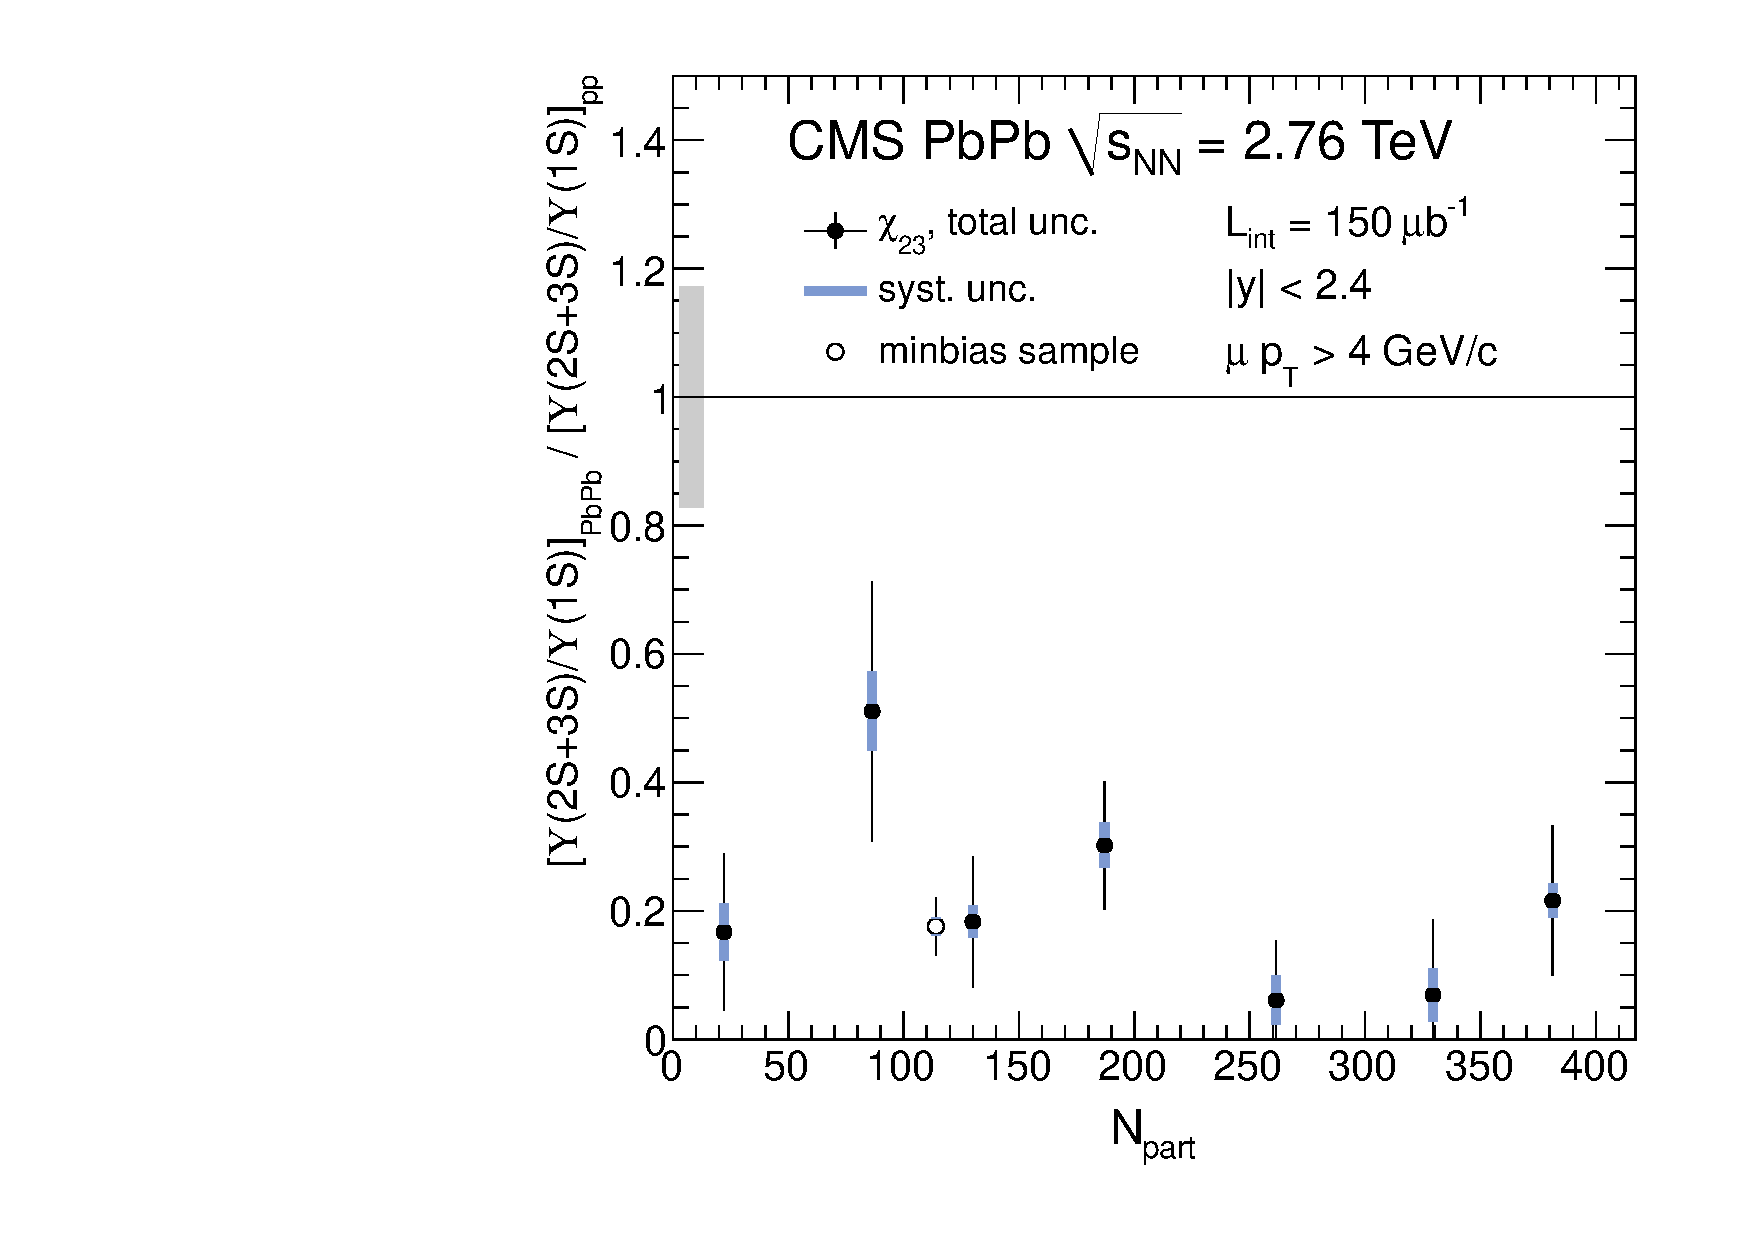
\includegraphics[angle=0,width=0.5\textwidth]{figures/fulldataset/chi23VsCent.pdf}}
    \subfigure[$\chi_{2}$, $\pt^\mu>4.0\GeVc$]{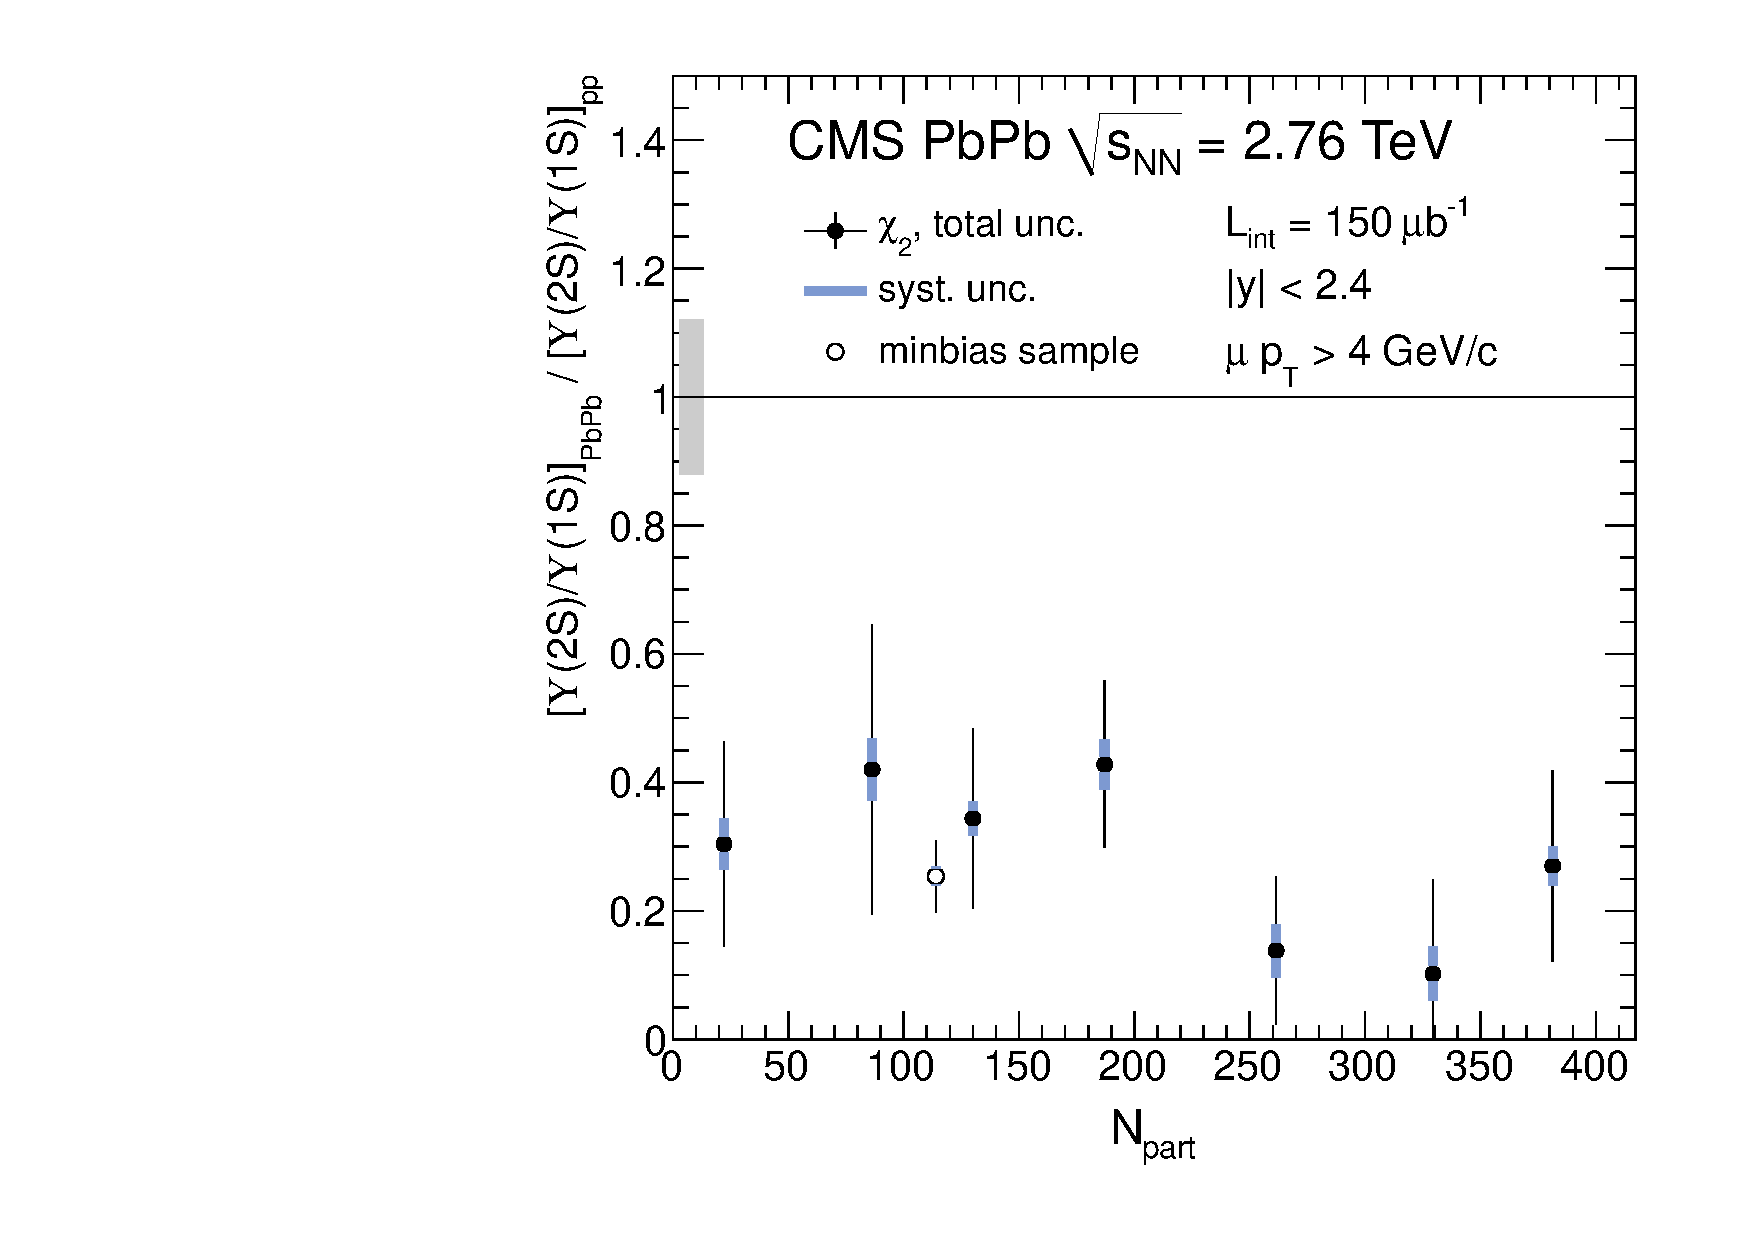
\includegraphics[angle=0,width=0.5\textwidth]{figures/fulldataset/chi2VsCent.pdf}}
    \caption{Centrality dependence of the double ratios $\chi_{23}$ and $\chi_{2}$;  %and nominal selection ($\pt^\mu>3.5\GeVc$); 
the PbPb statistical and systematic uncertainties are included; the graphs are normalized by the corresponding \pp single-ratio central values; \pp uncertainties are represented by gray box at unity, and are excluded from the data points as they do not affect point-to-point trend comparison. ($150 \mu b^{-1}$).}
    \label{fig:final_singlerat_centrality_nominal}
  \end{center}
\end{figure}

\begin{figure}[hbtp]
  \begin{center}
    \subfigure[$\chi_{23}$,$\pt^\mu>4.0\GeVc$]{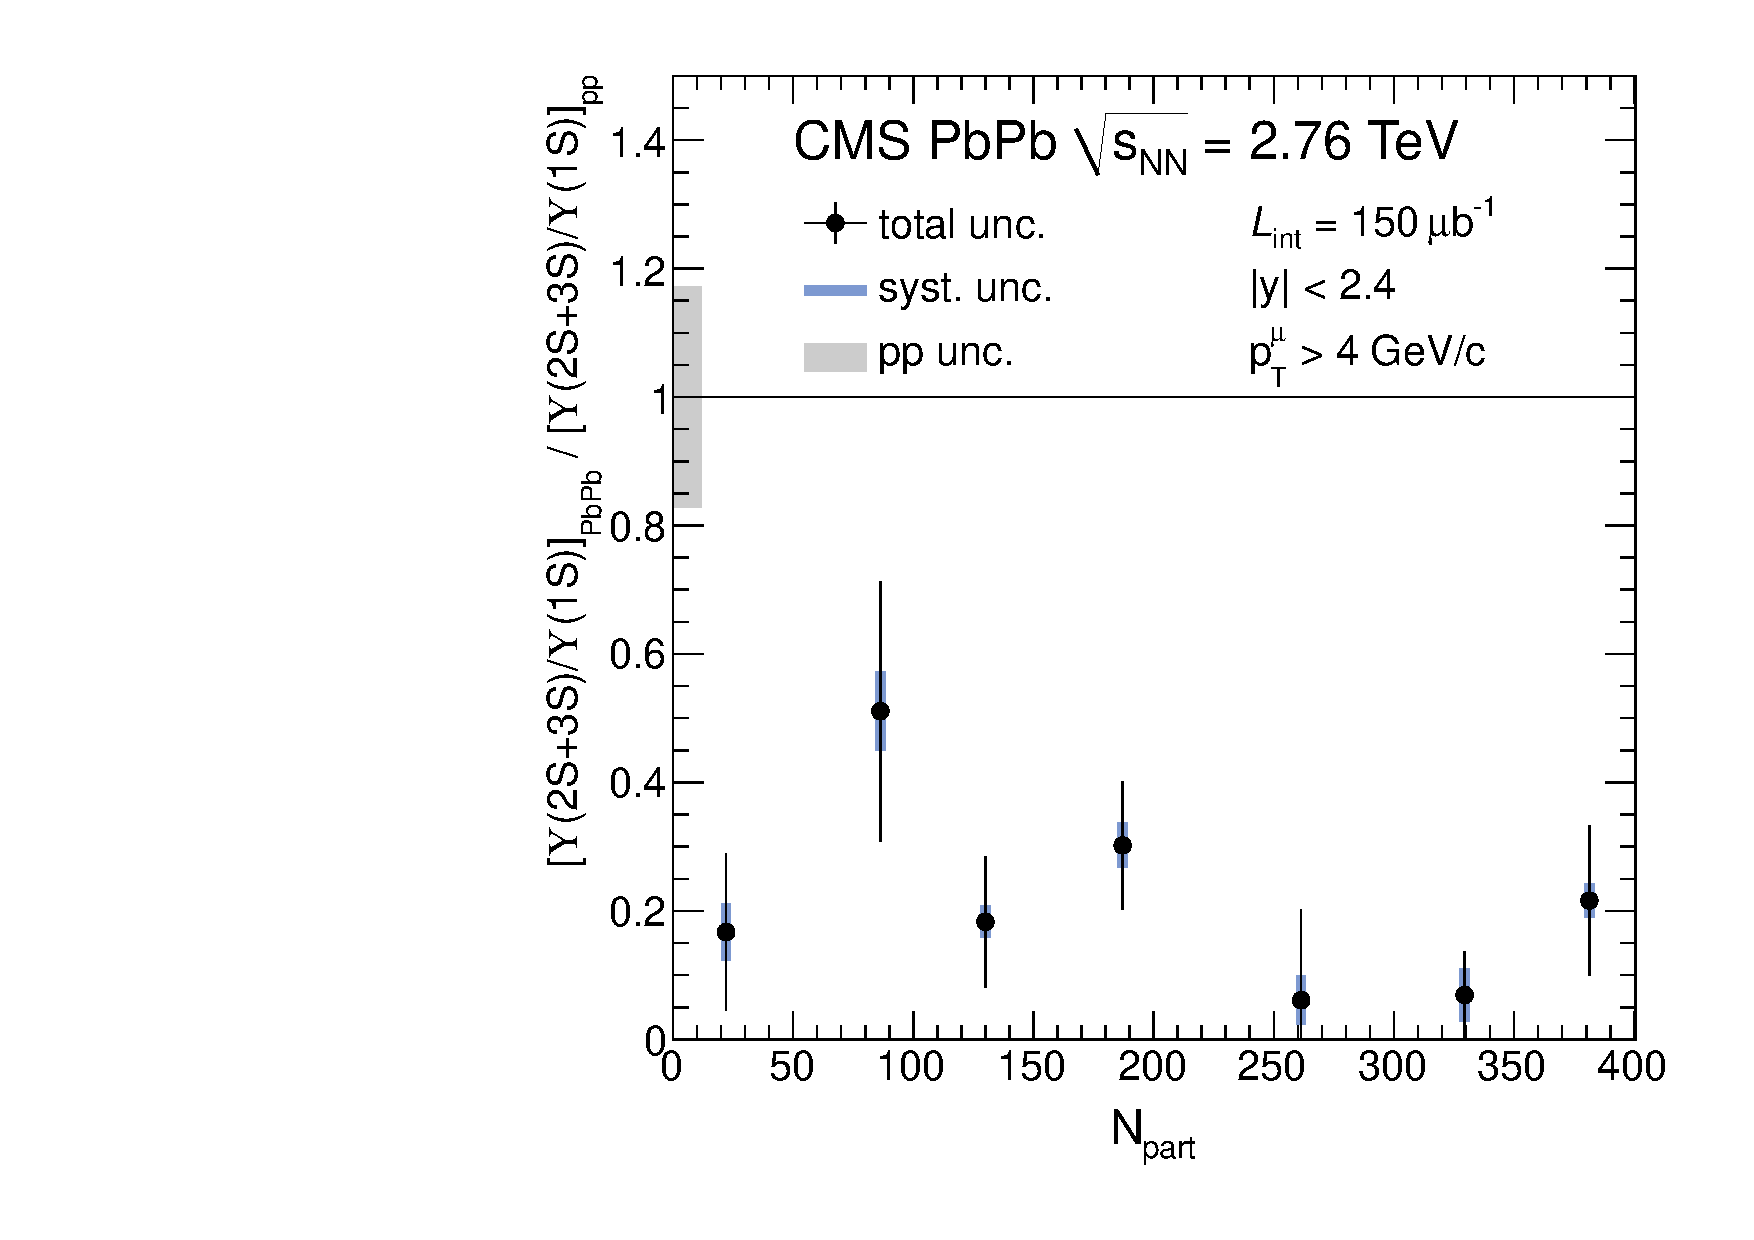
\includegraphics[angle=0,width=0.5\textwidth]{figures/fulldataset/chi23VsCent_limit.pdf}}
    \subfigure[$\chi_{2}$, $\pt^\mu>4.0\GeVc$]{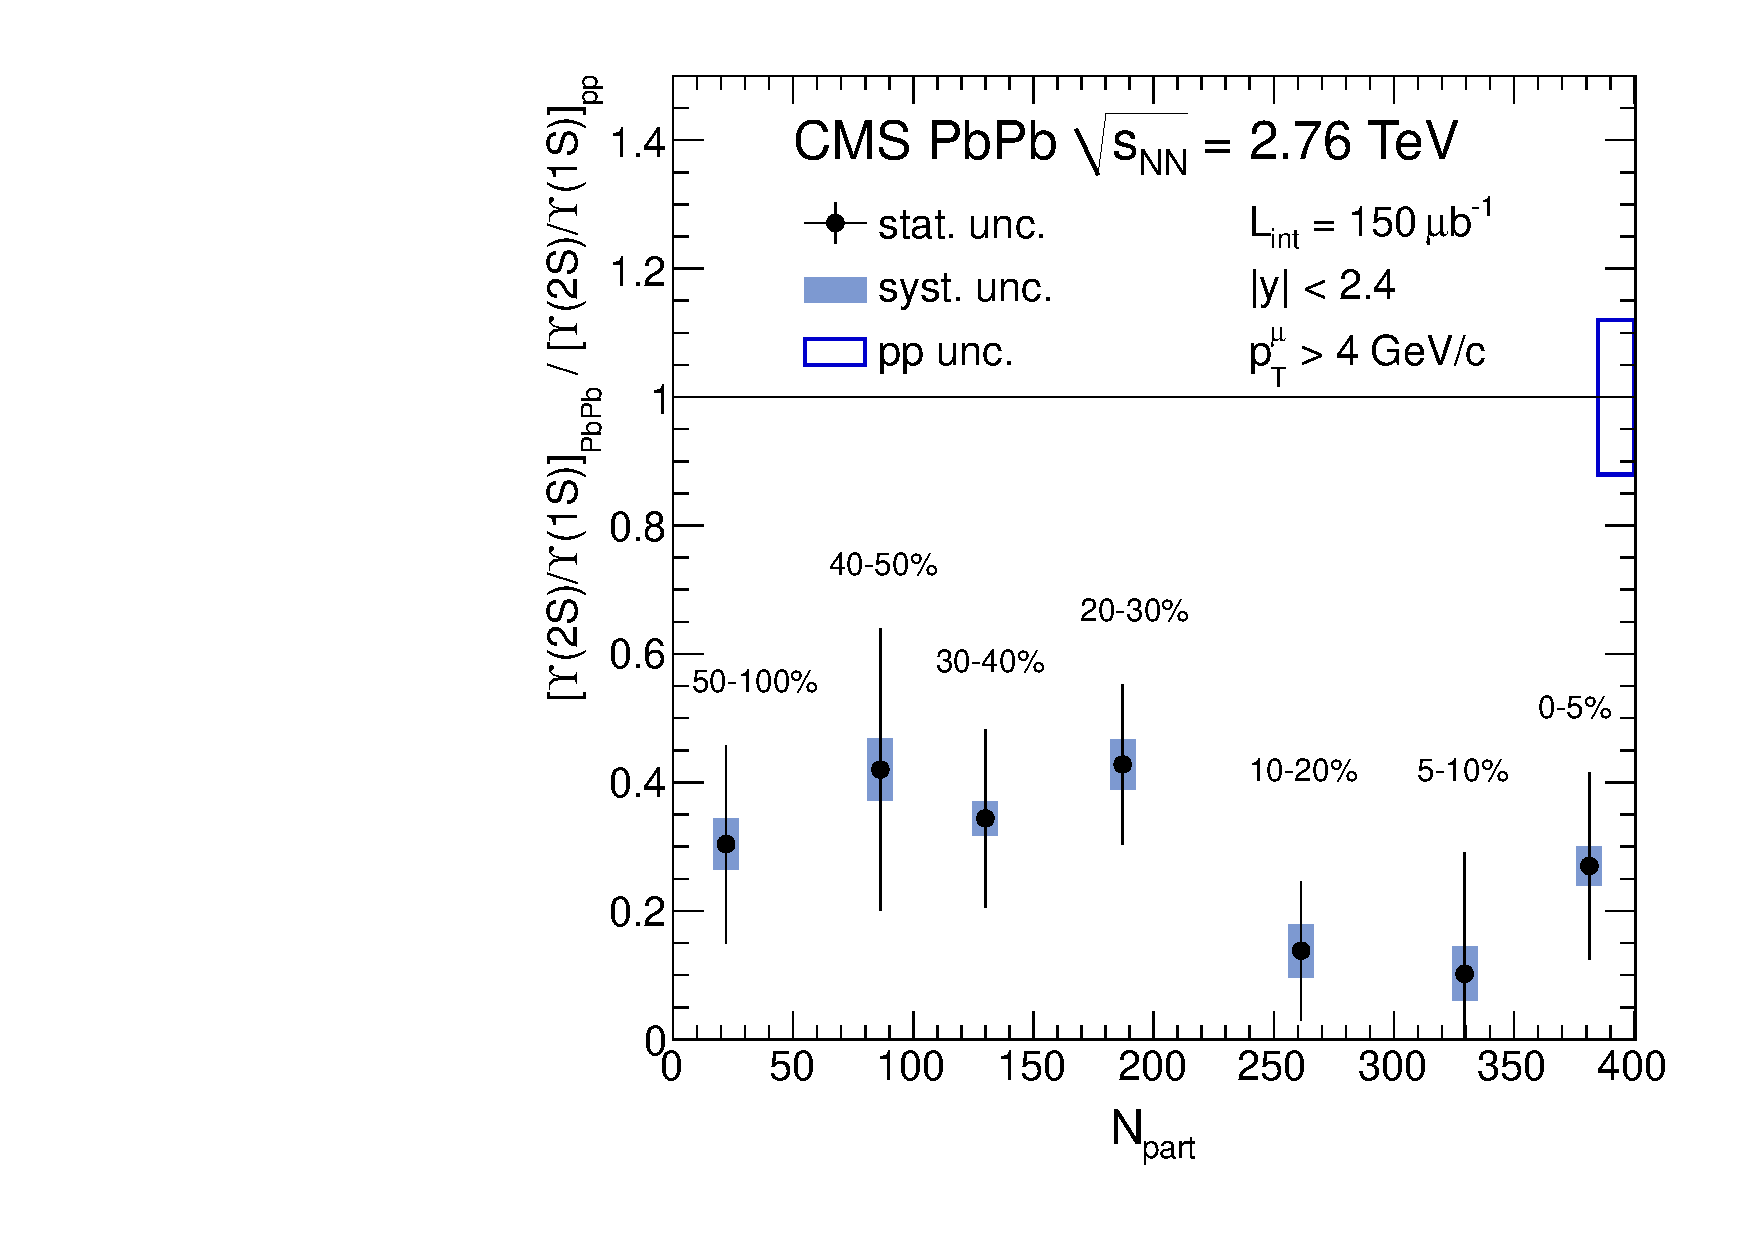
\includegraphics[angle=0,width=0.5\textwidth]{figures/fulldataset/chi2VsCent_limit.pdf}}
	\caption{Replace the negative error bars in \fig{fig:final_singlerat_centrality_nominal} with Feldman-Cousins limits.}
    \label{fig:final_singlerat_centrality_limit}
  \end{center}
\end{figure}


No clear dependence can be inferred within the statistical precision offered by the data. 
We also note that the most peripheral bin in \PbPb and the \pp reference do not necessarily match, both because a fully peripheral bin is not accessible given limited statistics in the data, and  
%Such basic behaviour can nonetheless be challenged, 
as a consequence of complexity of the underlying phenomena.  


\subsection{Double ratio measurement}

Here we study the comparison of the single ratios measured in PbPb and \Pp\Pp{}.
Such a double-ratio is given by 
%
\begin{linenomath}
\begin{eqnarray}
\label{eqn:x23:def}
\chi_{23} \equiv 
\frac{R_{23|\text{PbPb}}}{R_{23|\Pp\Pp}}
&=& \frac{
  [{N\left(\PgUb+\PgUc\right)}/{N(\PgUa)}]_{\text{PbPb}}
}{
  [{N\left(\PgUb+\PgUc\right)}/{N(\PgUa)}]_{\Pp\Pp}
} \,, \\
%
\label{eqn:x2:def}
\chi_{2} \equiv 
\frac{R_{2|\text{PbPb}}}{R_{2|\Pp\Pp}}
&=& \frac{
  [{N\left(\PgUb\right)}/{N(\PgUa)}]_{\text{PbPb}}
}{
  [{N\left(\PgUb\right)}/{N(\PgUa)}]_{\Pp\Pp}
} \,, \\
%
\label{eqn:x3:def}
\chi_{3} \equiv 
\frac{R_{3|\text{PbPb}}}{R_{3|\Pp\Pp}}
&=& \frac{
  [{N\left(\PgUc\right)}/{N(\PgUa)}]_{\text{PbPb}}
}{
  [{N\left(\PgUc\right)}/{N(\PgUa)}]_{\Pp\Pp}
} \,.
\end{eqnarray}
\end{linenomath}
%
No evidence for the $\PgUc$ state is found in the \PbPb data, and the corresponding ratio is studied in Sec.~\ref{sec:limits}. 

Several effects, and associated uncertainties, cancel out in the computation of these doubly normalized observables, including efficiency and acceptance correction factors. 
%between the resonance states in two samples, the ratios of the $R_{23}$ (Eqn.~(\ref{eqn:def:r23})) observables in PbPb and pp data 
%

The PbPb and \Pp\Pp{} data samples are fitted simultaneously, and the double ratios
%denoted below as $\chi_{23}$ and $\chi_{2}$, 
are directly extracted as fit parameters. 
%In the nominal fit configuration only the $\PgUa$ mass is commonly floated. 
%Identical signal models are applied to both datasets. 
The background is described by the nominal erf*exp model, in the case of the \PbPb dataset. 
For the \pp dataset, in view of the smaller statistics, a simpler background model is employed, namely a second order polynomial (that is, the same model and dataset as in previous publication~\cite{prl}).
%
The signal shape parameters are common, while the backgrounds float separately in the simultaneous fit. 
%
The fit projections are shown in Figures~\ref{fig:final_massfit_simultaneous_nominal_pt4}.

The double-ratio results and systematic uncertainties are summarized in Table~\ref{tab:final-doublerat-syst}.
For the signal fit function, we tried 7 different systematic variations (Table~\ref{tab:final-doublerat-syst}): 
\begin{itemize}
\item the CB signal tail parameters are fixed ($\alpha=1.4$, from high-statistics $\Pp\Pp$ data as in Table~\ref{tab:fsr})
\item the \PgUa mass resolution is fixed to Monte Carlo ($92$ \MeV)
\item fix both the CB parameters and mass resolution
\item let the CB tail float separately in pp and PbPb samples (it is shared for nominal)
\item let the resolution float separately in pp and PbPb samples (it is shared for nominal)
\item let both the CB tail and resolution float separately in pp and PbPb samples (they are shared for nominal)
\item share \PgUa mass mean in \pp and \PbPb samples (they float separately in the nominal configuration).
\end{itemize}

For the background function, we tried the following three sets of variations (Table~\ref{tab:final-doublerat-syst}):
\begin{itemize}
\item keep the second order polynomial for pp, but vary the PbPb fit with 4 different pdfs
\item keep the erf*exp function for PbPb, but vary the pp fit with 4 different pdfs
\item vary both PbPb and pp background pdfs at the same time
\end{itemize}

The systematic uncertainties associated to the signal and background modeling are estimated as the RMS, computed relative to the nominal fit value, for the corresponding set of variations described above. The total systematic uncertainty is obtained as the quadrature sum of these two sources. 
%of all the above variations with respect to the nominal value. 
%TBD: CORRECT STATEMENT AND TABLE: two partial RMS are computed, and added in quadrature in the end.
%A systematic uncertainty of 11\% is thus obtained for $\chi_{23}$ and of 7\% for $\chi_{2}$, as 
The systematic uncertainties on the double ratios are detailed in Table~\ref{tab:final-doublerat-syst}. 

\begin{figure}[hbtp]
  \begin{center}
    \subfigure[\PbPb projection]{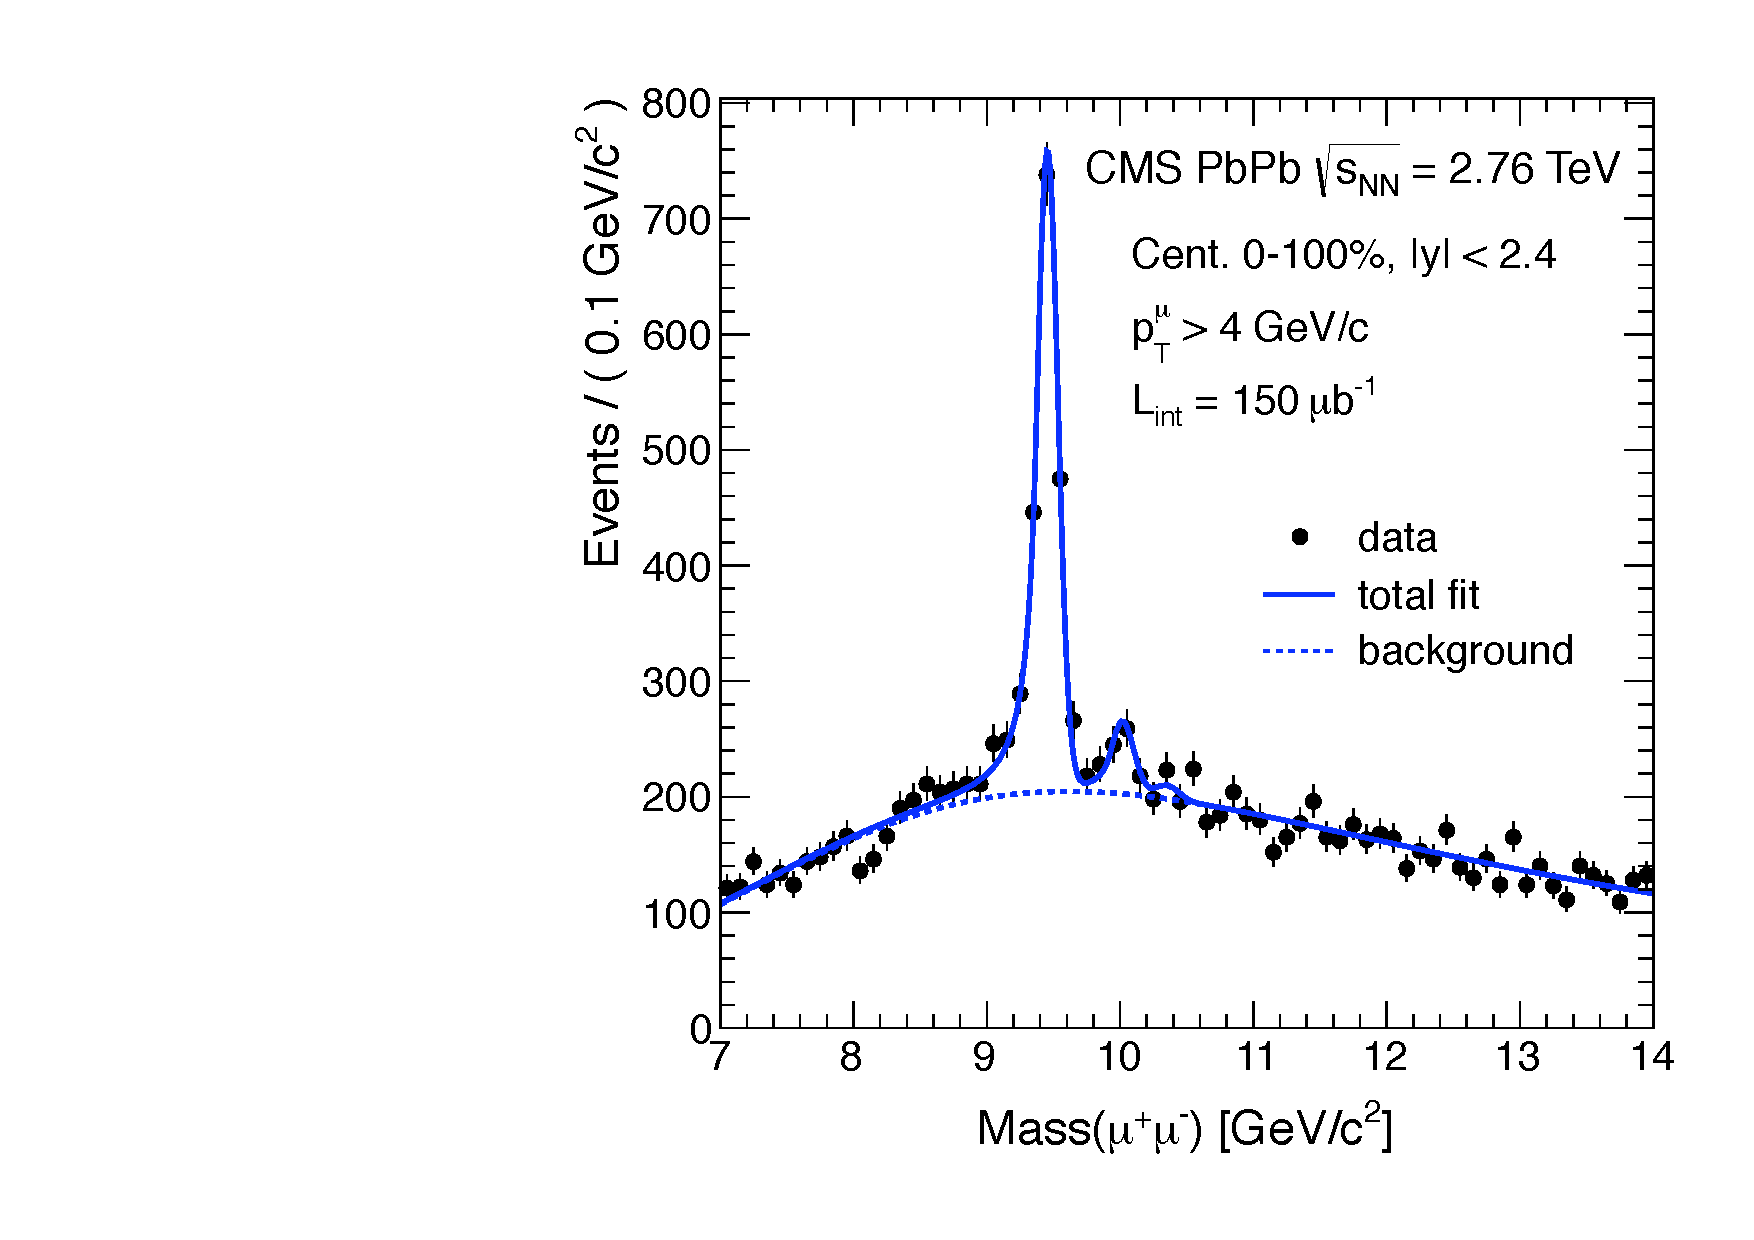
\includegraphics[angle=0,width=0.5\textwidth]{figures/fulldataset/hiFitPt40}}
    \subfigure[\pp   projection]{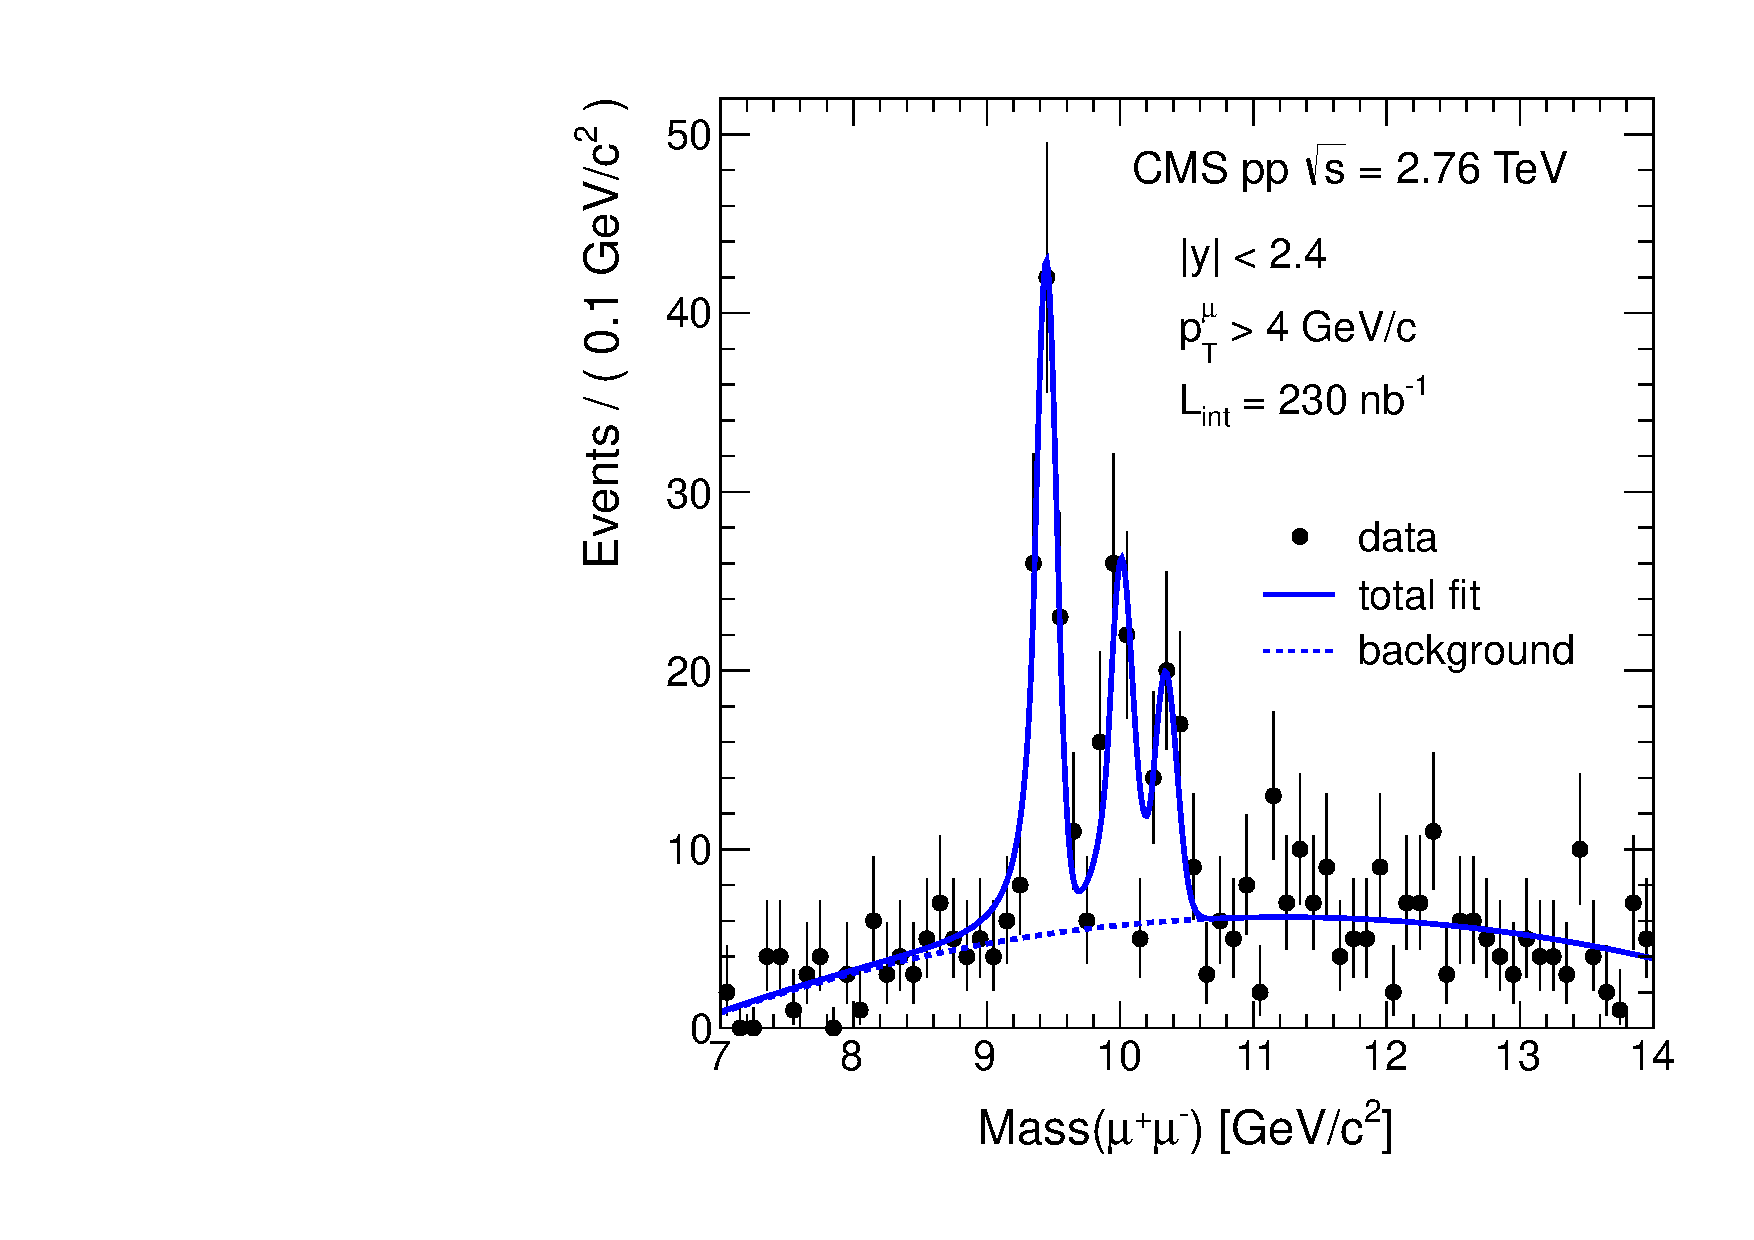
\includegraphics[angle=0,width=0.5\textwidth]{figures/fulldataset/ppFitPt40}}
    \caption{Simultaneous fit to the \PbPb  ($150 \mu b^{-1}$) and \pp ($231 nb^{-1}$) datasets, for $\pt^\mu>4.0\GeVc$.}
    \label{fig:final_massfit_simultaneous_nominal_pt4}
  \end{center}
\end{figure}

\begin{table}[!h]
  \centering
  \caption{Double-ratio results.}
  \begin{tabular}{ll|c|c|c}
    \hline
\multicolumn{2}{c|}{} &\multicolumn{3}{c}{$\pt^\mu>4.0\GeVc$, Cent. 0-100\%} \\ 
\multicolumn{2}{c|}{} &       $\chi_{23}$       &       $\chi_{2}$        &     $\chi_{3}$    \\
\hline
\multicolumn{2}{l|}{nominal result}                    & $0.15\pm 0.05$  & $0.21\pm 0.07$  &  $0.06\pm 0.06$   \\
\hline \hline
\multicolumn{4}{l}{signal pdf systematic variations:} \\
\multicolumn{2}{l|}{fix CB tail to MC}                 & $0.135\pm 0.047$  & $0.200\pm 0.066$    &  $0.063\pm 0.054$ \\
\multicolumn{2}{l|}{fix resolution to MC}              & $0.153\pm 0.049$  & $0.217\pm 0.070$    &  $0.081\pm 0.063$ \\
\multicolumn{2}{l|}{fix CB and resolution to MC}       & $0.144\pm 0.047$  & $0.207\pm 0.067$    &  $0.000\pm 0.000$ \\ 
\multicolumn{2}{l|}{separated floating CB tail}        & $0.166\pm 0.052$  & $0.226\pm 0.070$    &  $0.098\pm 0.058$ \\
\multicolumn{2}{l|}{separated floating resolution}     & $0.149\pm 0.048$  & $0.215\pm 0.070$    &  $0.080\pm 0.064$ \\
\multicolumn{2}{l|}{separated CB tail and resolution}  & $0.163\pm 0.048$  & $0.223\pm 0.064$    &  $0.098\pm 0.063$ \\
\multicolumn{2}{l|}{shared mean}                       & $0.150\pm 0.048$  & $0.219\pm 0.064$    &  $0.076\pm 0.062$ \\
\hline \hline
\multicolumn{4}{l}{background pdf systematic variations:} \\
PbPb model & pp model & & & \\
LS erf*exp + pol.2;     & pol.2 & $0.157\pm0.047$ & $0.220\pm0.070$  &  $0.075\pm 0.064$ \\
LS keys + pol.2;        & pol.2 & $0.161\pm0.049$ & $0.223\pm0.071$  &  $0.040\pm 0.061$ \\
OS TrkRot erf*exp + pol.2; & pol.2 & $0.157\pm0.047$ & $0.221\pm0.070$  &  $0.094\pm 0.067$ \\
OS TrkRot keys + pol.2;    & pol.2 & $0.164\pm0.050$ & $0.215\pm0.069$  &  $0.070\pm 0.062$ \\
%LS TrkRot erf*exp + pol.2; & pol.2 & $0.170\pm0.049$ & $0.236\pm0.072$ \\
%LS TrkRot keys + pol.2;    & pol.2 & $0.168\pm0.048$ & $0.232\pm0.072$ \\
\hline
LS keys + pol.2;        & LS keys + pol.2    & $0.167\pm0.053$ & $0.234\pm0.076$  &  $0.042\pm 0.065$ \\
LS erf*exp + pol.2;     & LS erf*exp + pol.2 & $0.158\pm0.048$ & $0.222\pm0.071$  &  $0.075\pm 0.046$ \\
\hline
erf*exp;                & erf*exp            & $0.153\pm0.050$ & $0.219\pm0.071$  &  $0.079\pm 0.068$ \\
erf*exp;                & erf*exp(shared erf)& $0.143\pm0.045$ & $0.216\pm0.066$  &  $0.070\pm 0.062$ \\
erf*exp;                & LS erf*exp + pol.2 & $0.148\pm0.049$ & $0.215\pm0.071$  &  $0.075\pm 0.046$ \\
erf*exp;                & LS keys + pol.2    & $0.155\pm0.043$ & $0.224\pm0.063$  &  $0.081\pm 0.069$ \\
\hline \hline
\multicolumn{4}{l}{Total systematic from fit (RMS of all the fit variations):} \\
%\multicolumn{2}{l|}{Fit relative systematic} & 8.6\%  & 5.1\%  \\  %LS TrkRot
%\multicolumn{2}{l|}{Fit absolute systematic} & 0.012 & 0.011 \\   %LS TrkRot
\multicolumn{2}{l|}{Fit relative systematic} & 7.6\%  & 4.0\%  & 46.8\% \\  %OS TrkRot
\multicolumn{2}{l|}{Fit absolute systematic} & 0.01 & 0.01 & 0.03\\    %OS TrkRot
\hline
\multicolumn{4}{l}{Total systematic from fit(take the largest one from equivalent variations):} \\
\multicolumn{2}{l|}{Fit relative systematic} & 19.3\%  & 11.7\%  & 100.6\%\\
\multicolumn{2}{l|}{Fit absolute systematic} & 0.03 & 0.02 & 0.06 \\
%\multicolumn{2}{l|}{Fit relative systematic} & 13.6\%  & 9.4\%  \\ %OS TrkRot
%\multicolumn{2}{l|}{Fit absolute systematic} & 0.021 & 0.020 \\    %OS TrkRot
\hline
\hline
\multicolumn{2}{l|}{systematic from efficiency} & 1.0\% & 1.0\% & 1.0\%\\
\hline \hline
\multicolumn{4}{l}{Total systematic: } \\
\multicolumn{2}{l|}{Total relative systematic} & 19.3\%  & 11.8\%  &100.6\% \\
\multicolumn{2}{l|}{Total absolute systematic} & 0.03 & 0.02 & 0.06\\
\hline \hline
\multicolumn{4}{l}{other checks:} \\
LS TrkRot erf*exp + pol.2; & pol.2 & $0.170\pm0.049$ & $0.236\pm0.072$   & $0.061 \pm 0.080$\\
LS TrkRot keys + pol.2;    & pol.2 & $0.168\pm0.048$ & $0.232\pm0.072$   & $0.088 \pm 0.066$\\
%OS TrkRot erf*exp + pol.2; & pol.2 & $0.157\pm0.047$ & $0.221\pm0.070$ \\
%OS TrkRot keys + pol.2;    & pol.2 & $0.164\pm0.050$ & $0.215\pm0.069$ \\
\hline
\end{tabular}
  \label{tab:final-doublerat-syst}
\end{table}

%\end{document}

%\clearpage

\subsection{Kinematic dependences}

The single-ratio and double-ratio measurements are performed in bins of dimuon rapidity and transverse momentum, %based on the PbPb dataset and 7 TeV pp dataset, 
for the nominal ($\pt>4.0 \GeVc$) selection. 
The fits to the data are shown in Figures~\ref{fig:final_massfit_singlerat_ptdif} and~\ref{fig:final_massfit_singlerat_rapdif}.
The background level and shape are seen to vary considerably in the different regions, as expected. 
For example, the kinematic effect due to the muon \pt{} selection threshold is more noticeable for low dimuon \pt{} and high rapidity regions, with softer muon \pt{} spectra. 

The double-ratio results are represented in the graphs in \fig{fig:final_doublerat_differential}. 
Due to the limitted statistics in the \pp sample, the statistical precision available does not allow to infer possible dependencies of the double ratio on the inspected kinematic variables. 

\begin{figure}[hbtp]
  \begin{center}
    \subfigure[\PbPb data $0.0<|y|<1.0$]{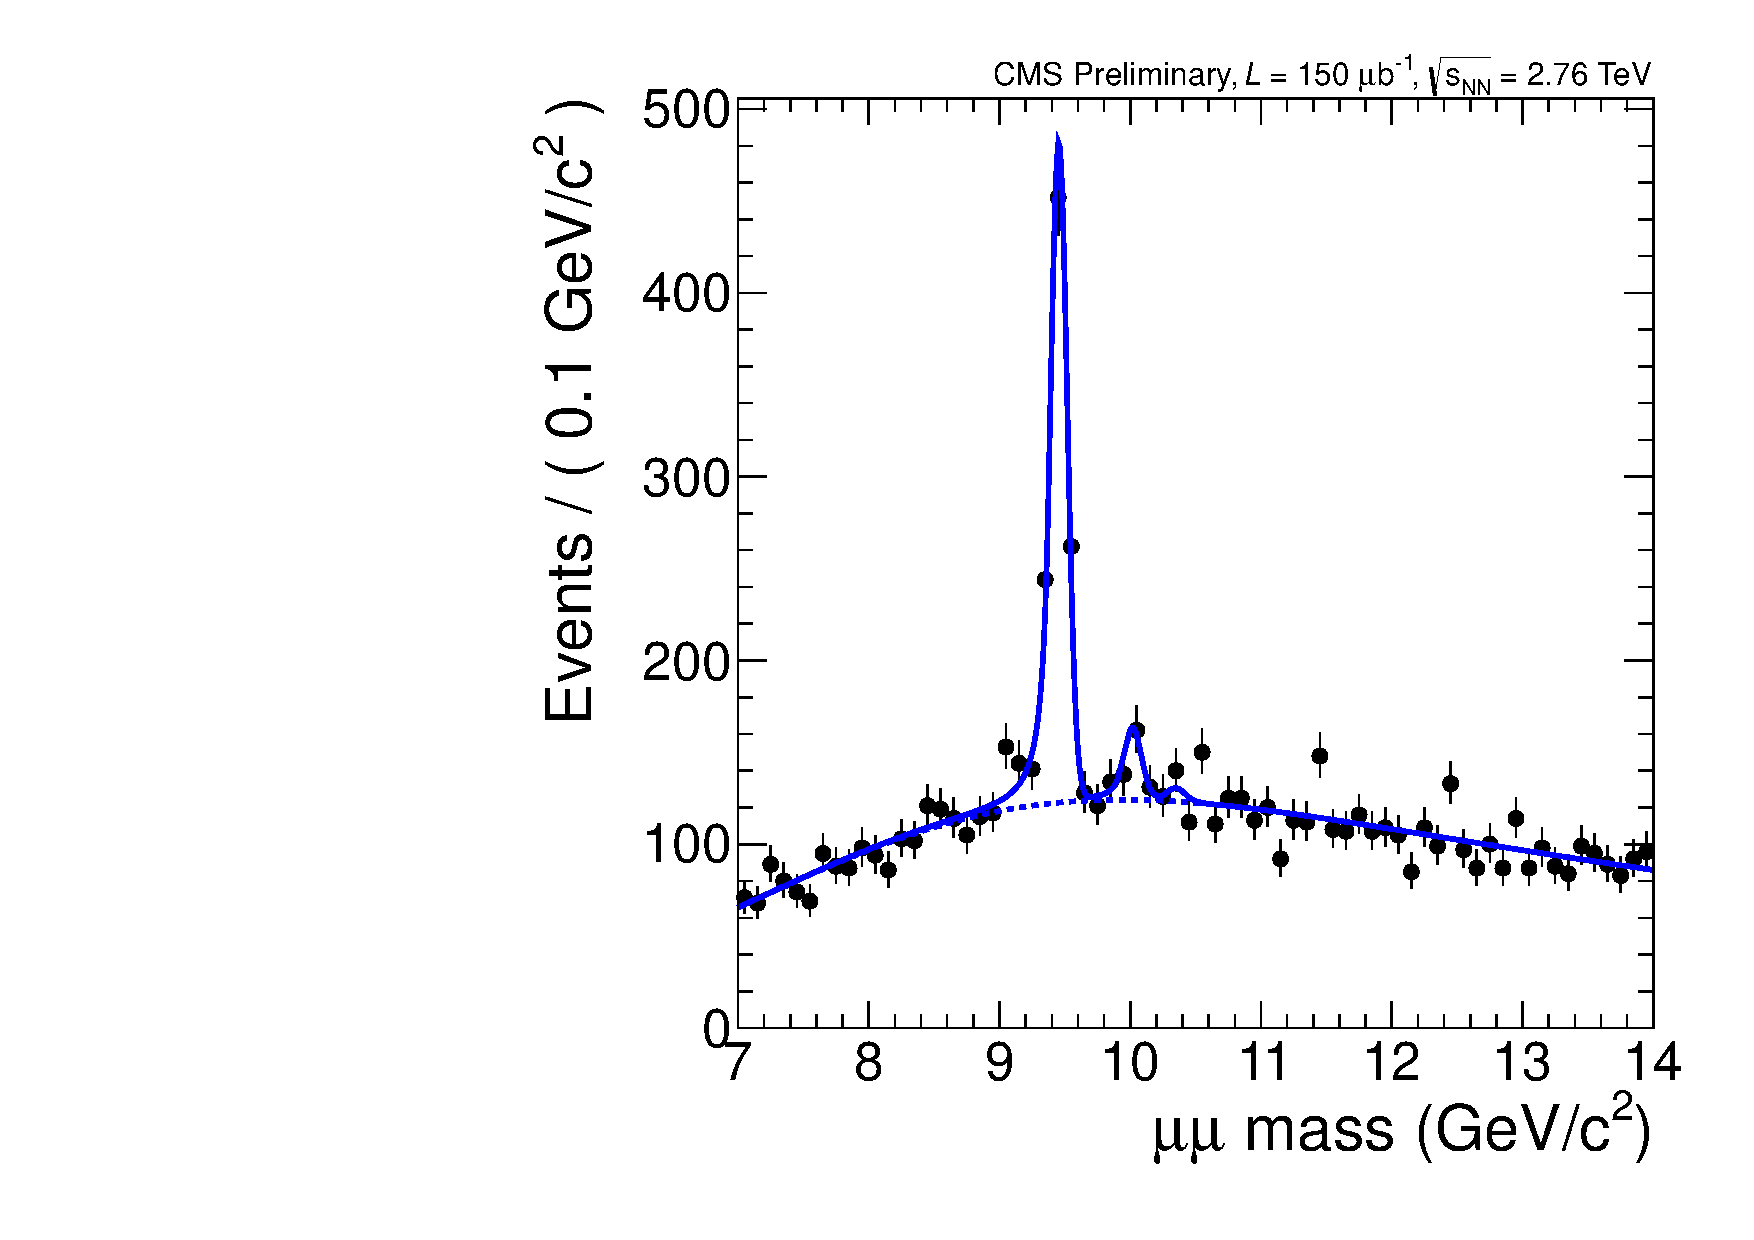
\includegraphics[angle=0,width=0.45\textwidth]{figures/pt_rapidity/hiFitPt4rap1}}
    \subfigure[\pp   data $0.0<|y|<1.0$]{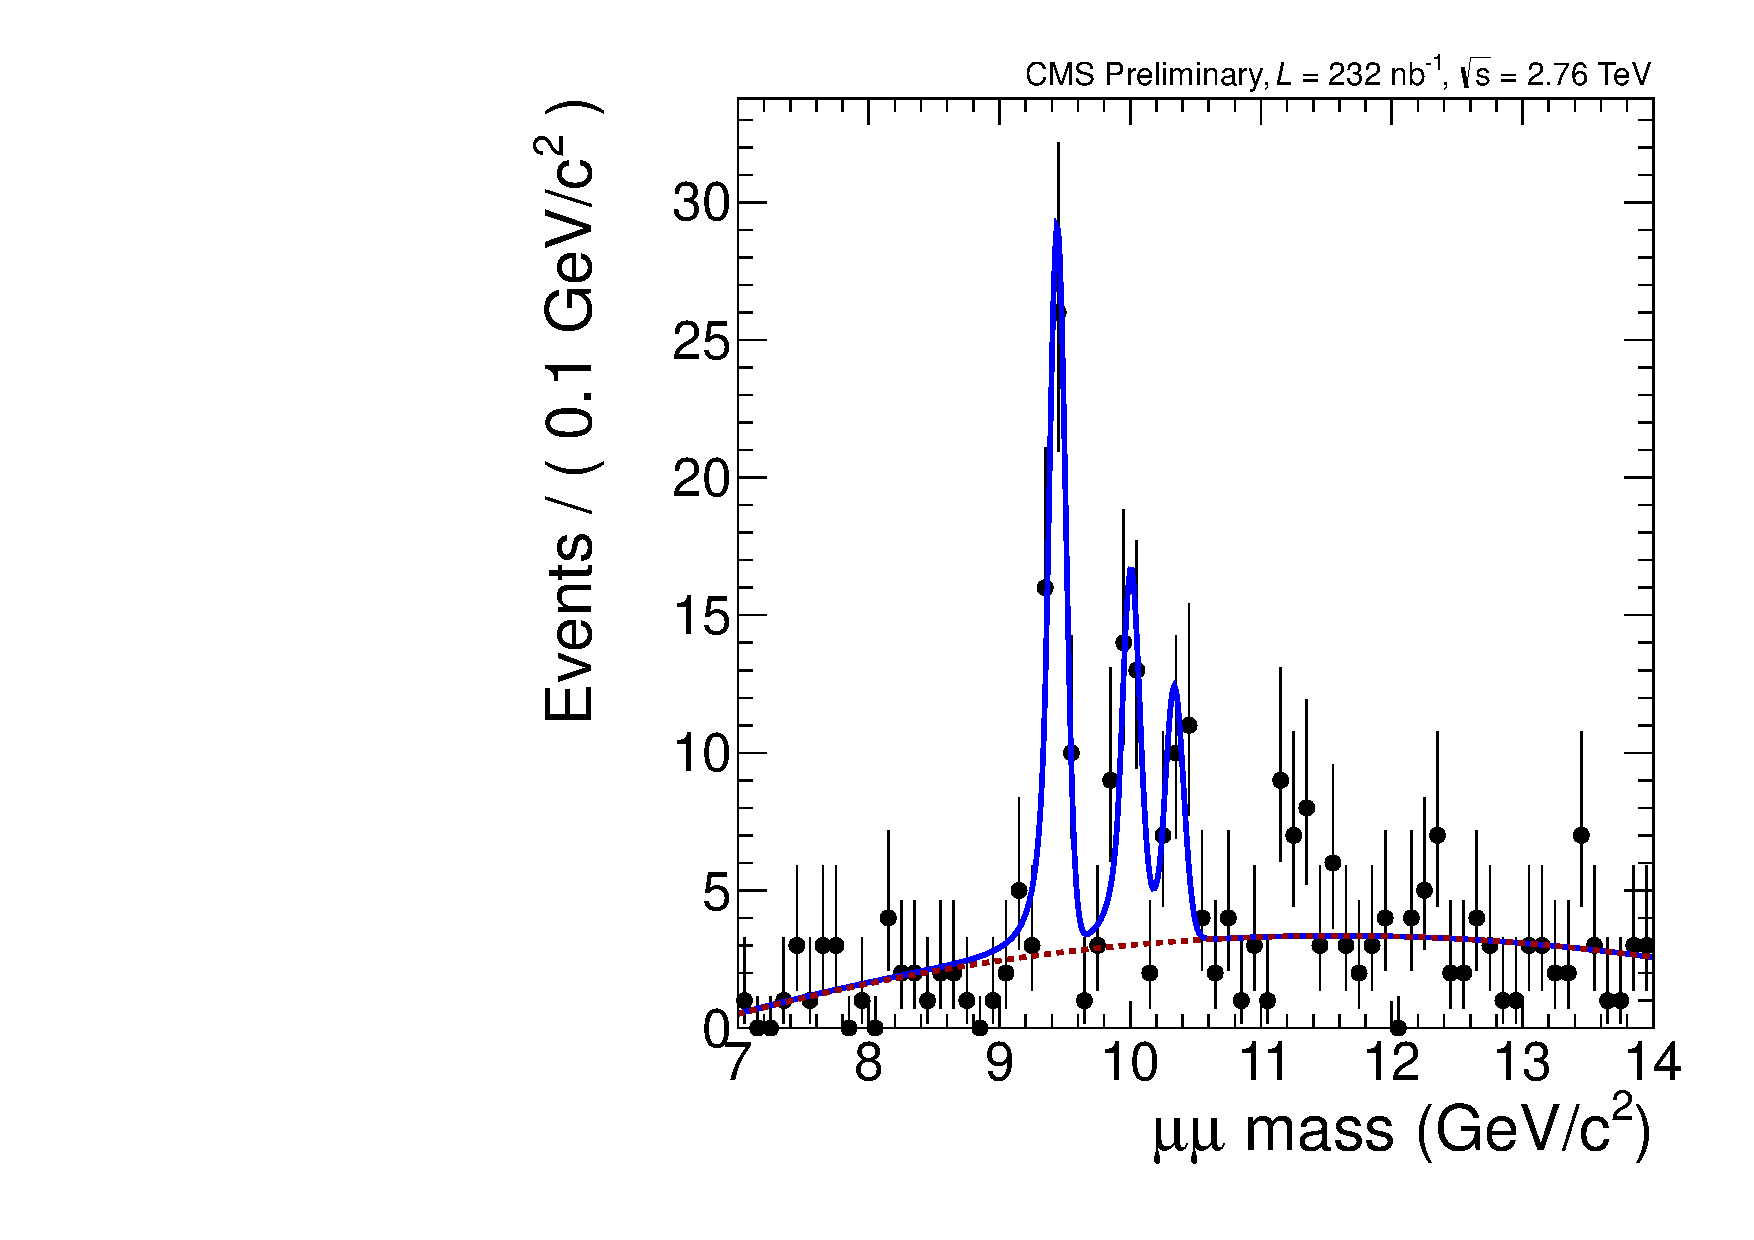
\includegraphics[angle=0,width=0.45\textwidth]{figures/pt_rapidity/ppFitPt4rap1}} \\
    \subfigure[\PbPb data $1.0<|y|<2.4$]{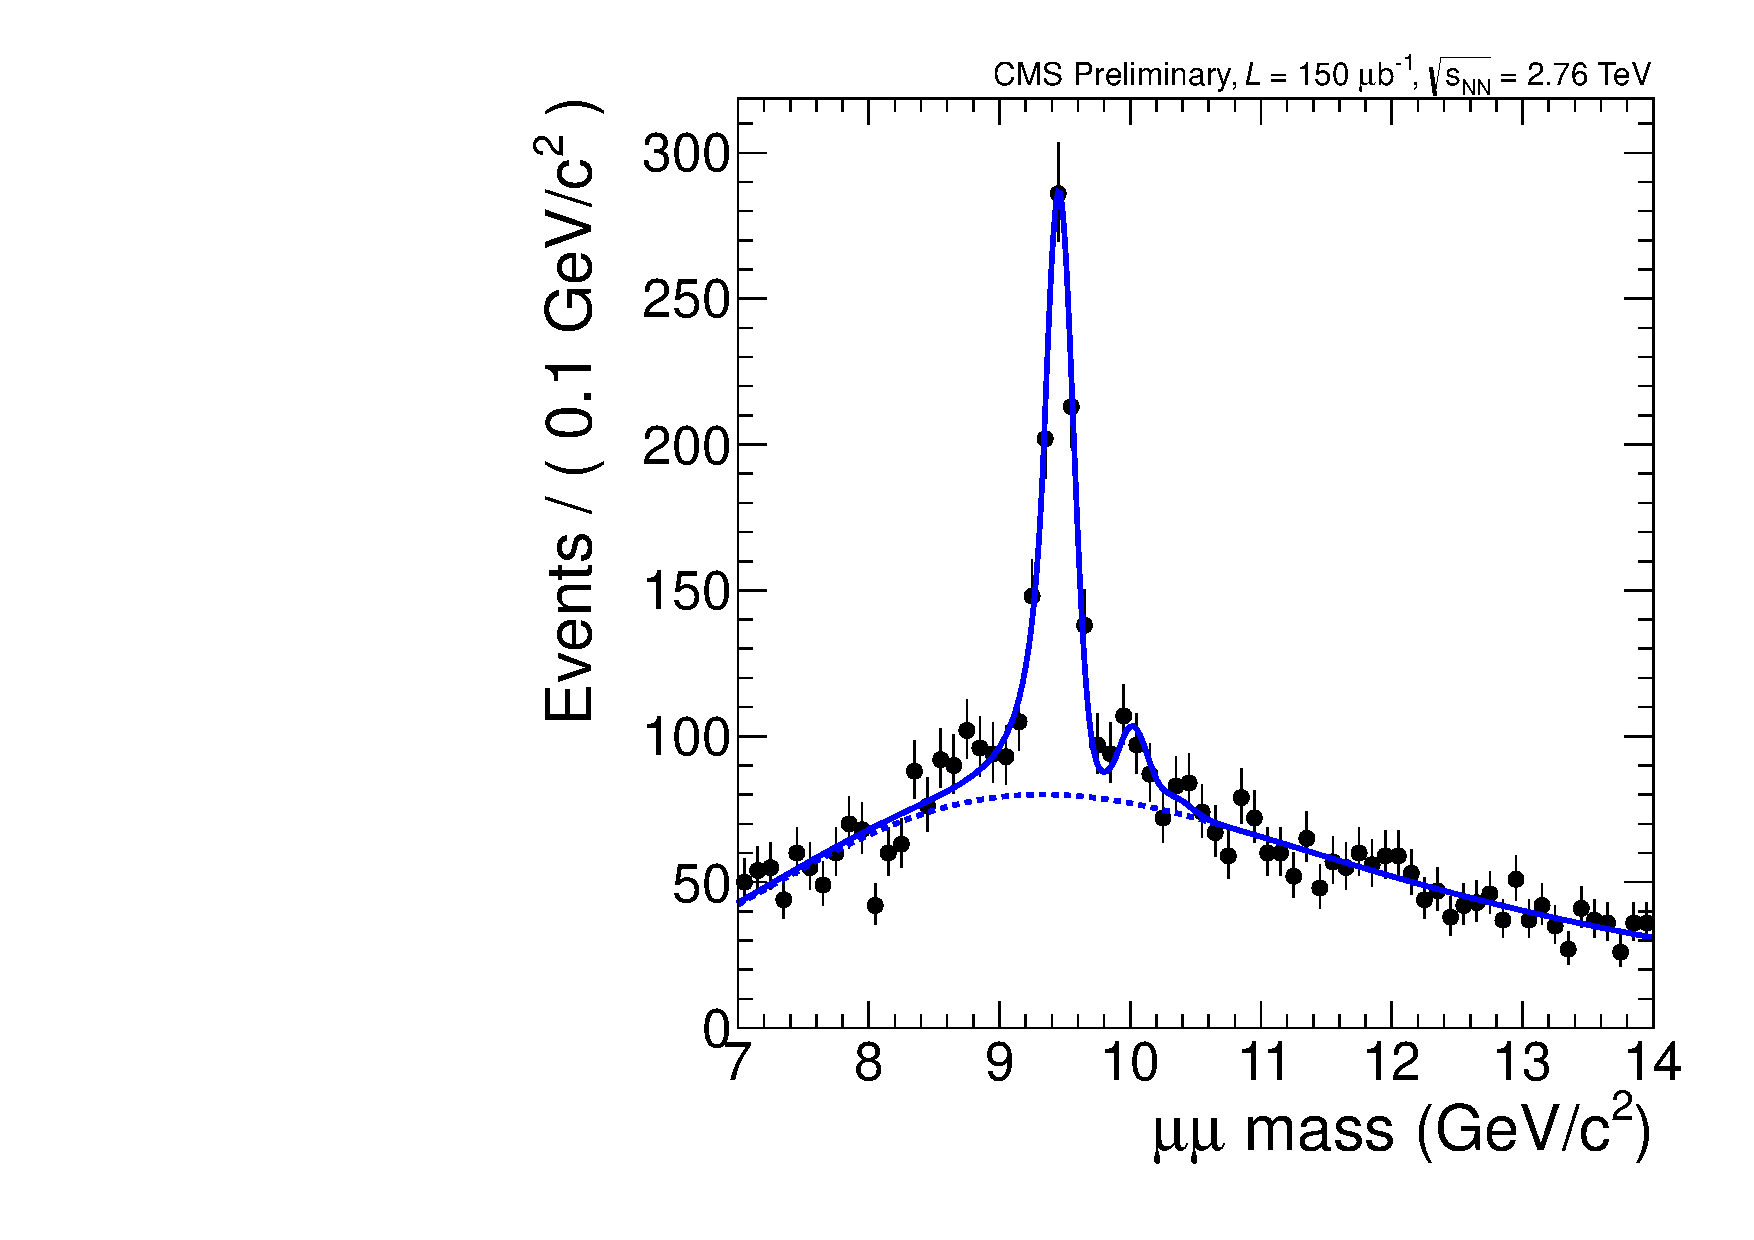
\includegraphics[angle=0,width=0.45\textwidth]{figures/pt_rapidity/hiFitPt4rap2}}
    \subfigure[\pp   data $1.0<|y|<2.4$]{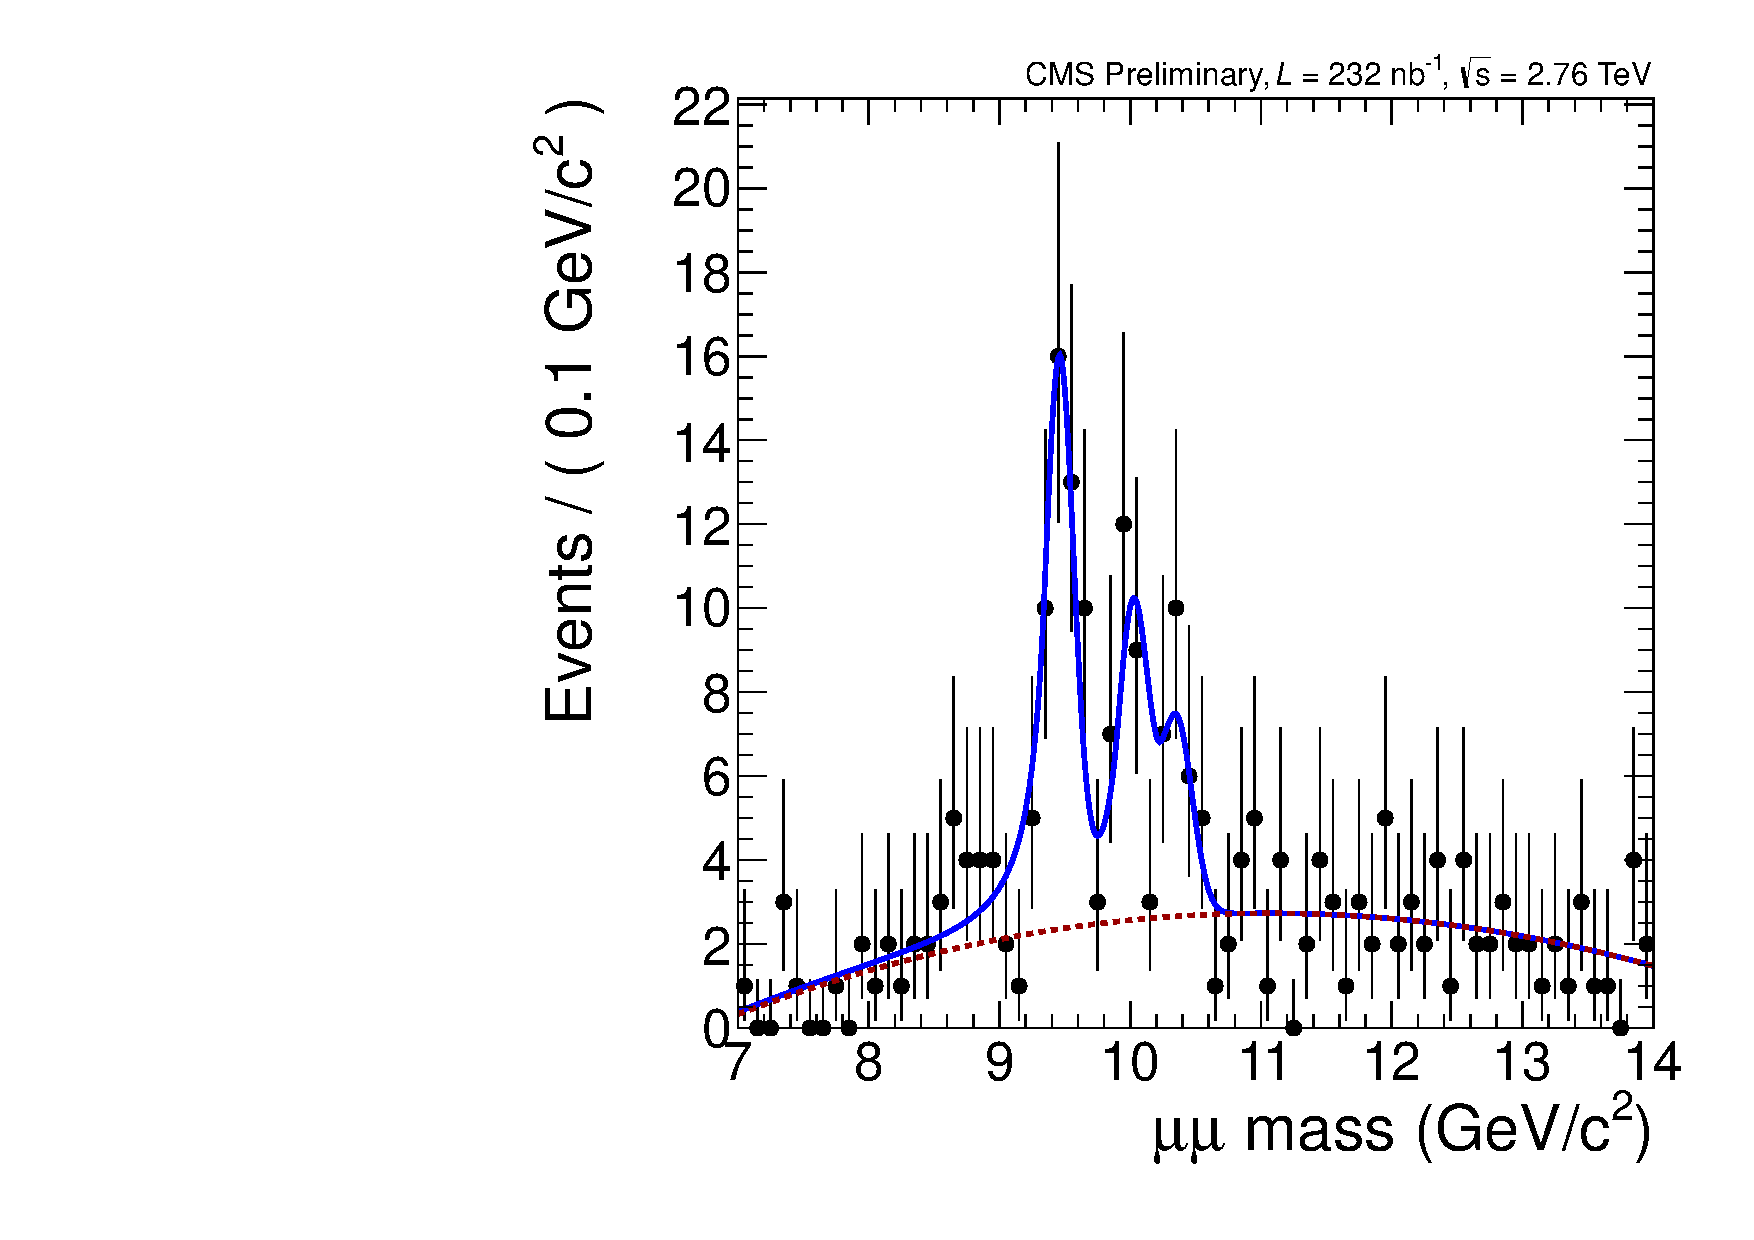
\includegraphics[angle=0,width=0.45\textwidth]{figures/pt_rapidity/ppFitPt4rap2}}
  \caption{Mass fits in ranges of dimuon rapidity.}
  \label{fig:final_massfit_singlerat_ptdif}
  \end{center}
\end{figure}

\begin{figure}[hbtp]
  \begin{center}
    \subfigure[\PbPb data $\pt^\PgU<5\GeVc$]{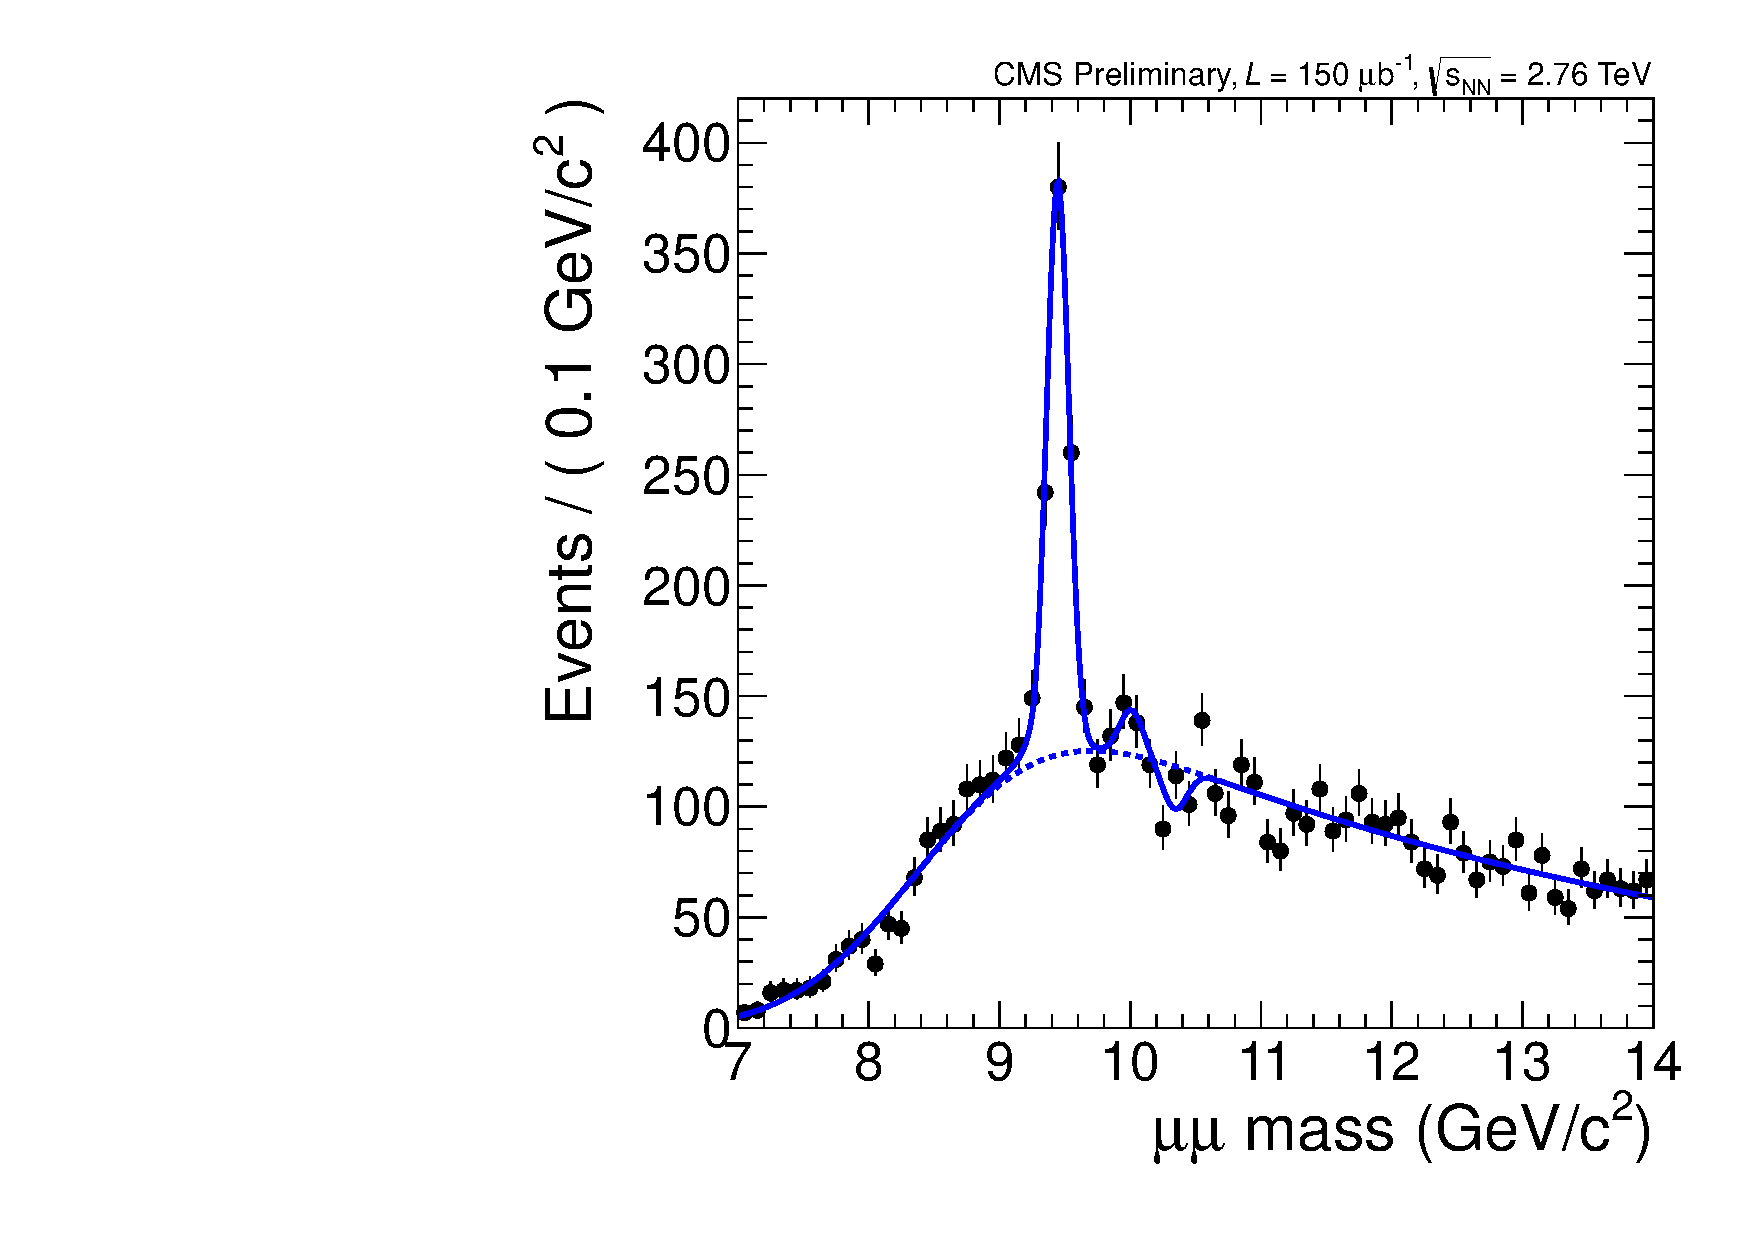
\includegraphics[angle=0,width=0.45\textwidth]{figures/pt_rapidity/hiFitPt4pt1}}
    \subfigure[\pp   data $\pt^\PgU<5\GeVc$]{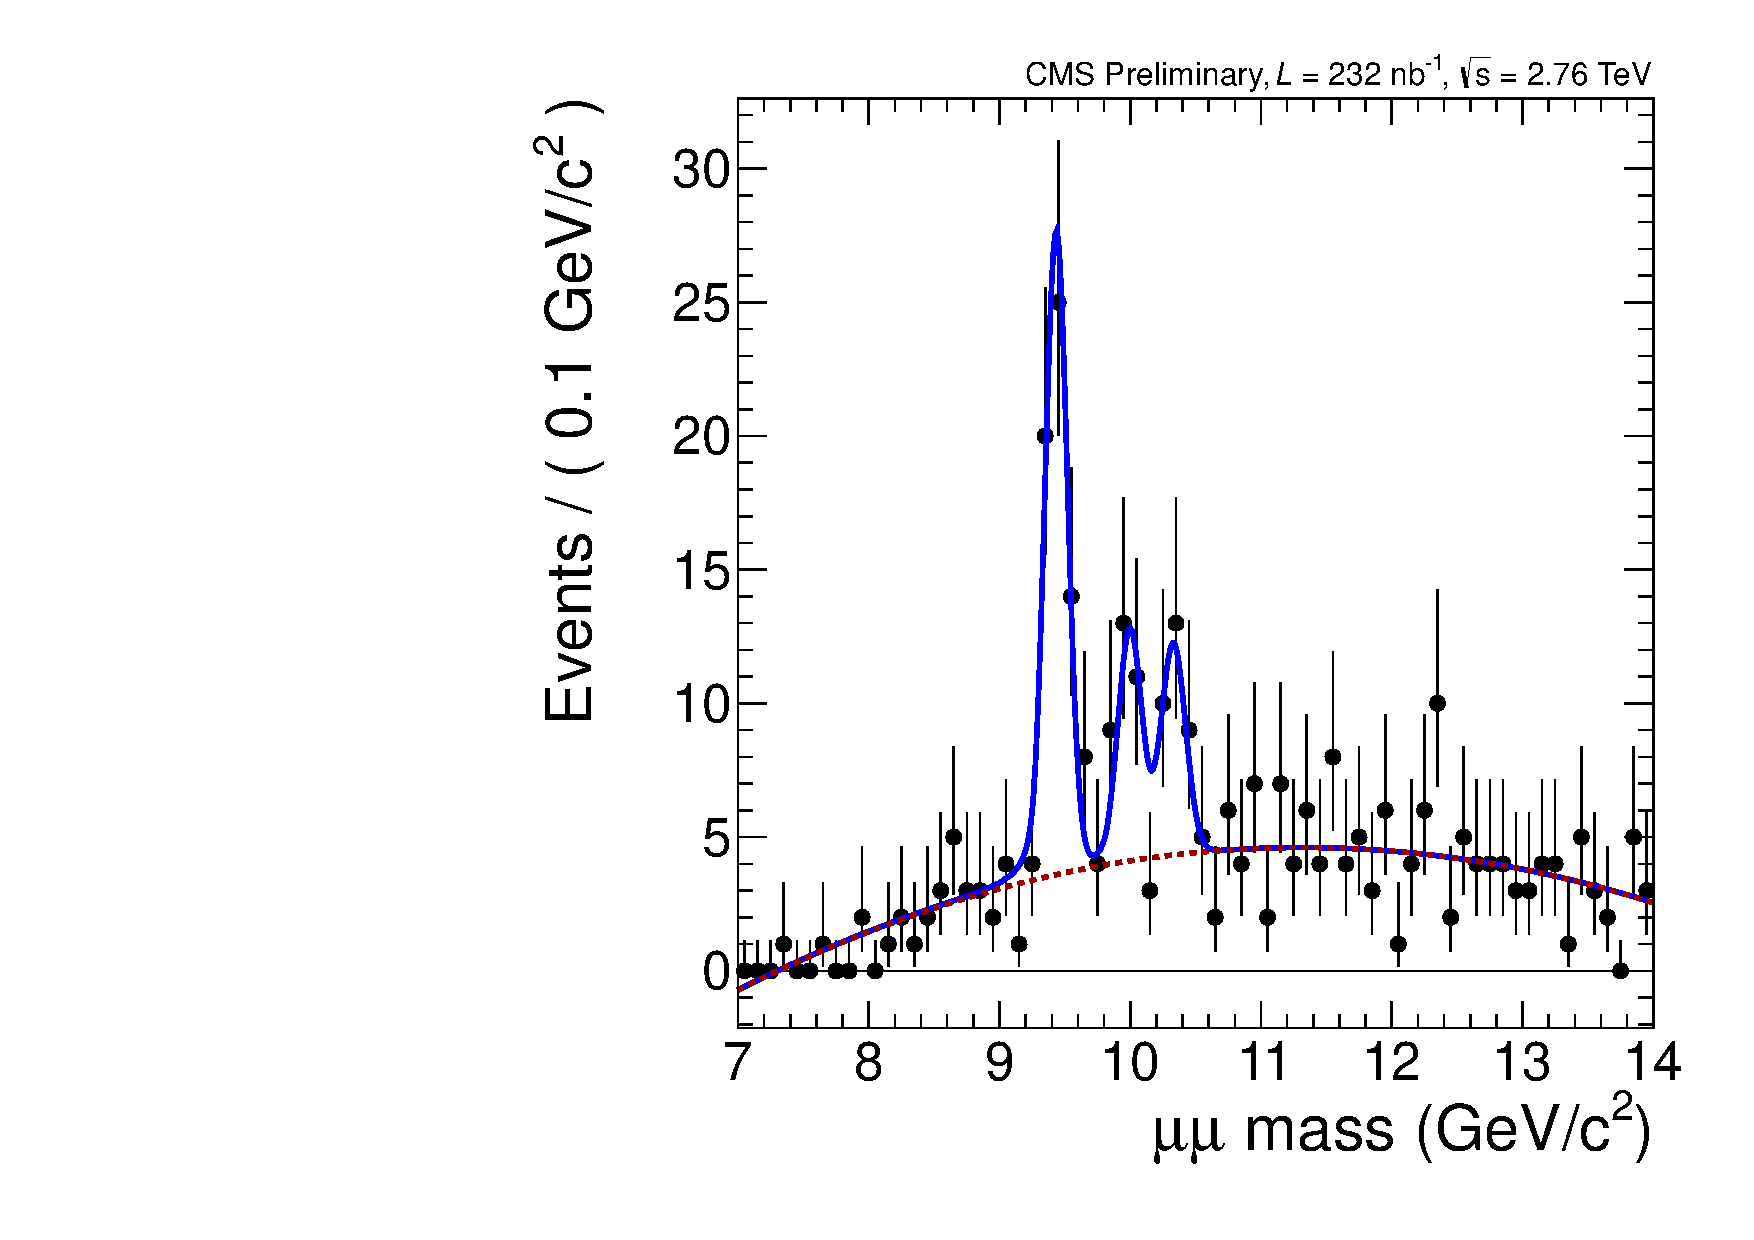
\includegraphics[angle=0,width=0.45\textwidth]{figures/pt_rapidity/ppFitPt4pt1}} \\
    \subfigure[\PbPb data $\pt^\PgU>5\GeVc$]{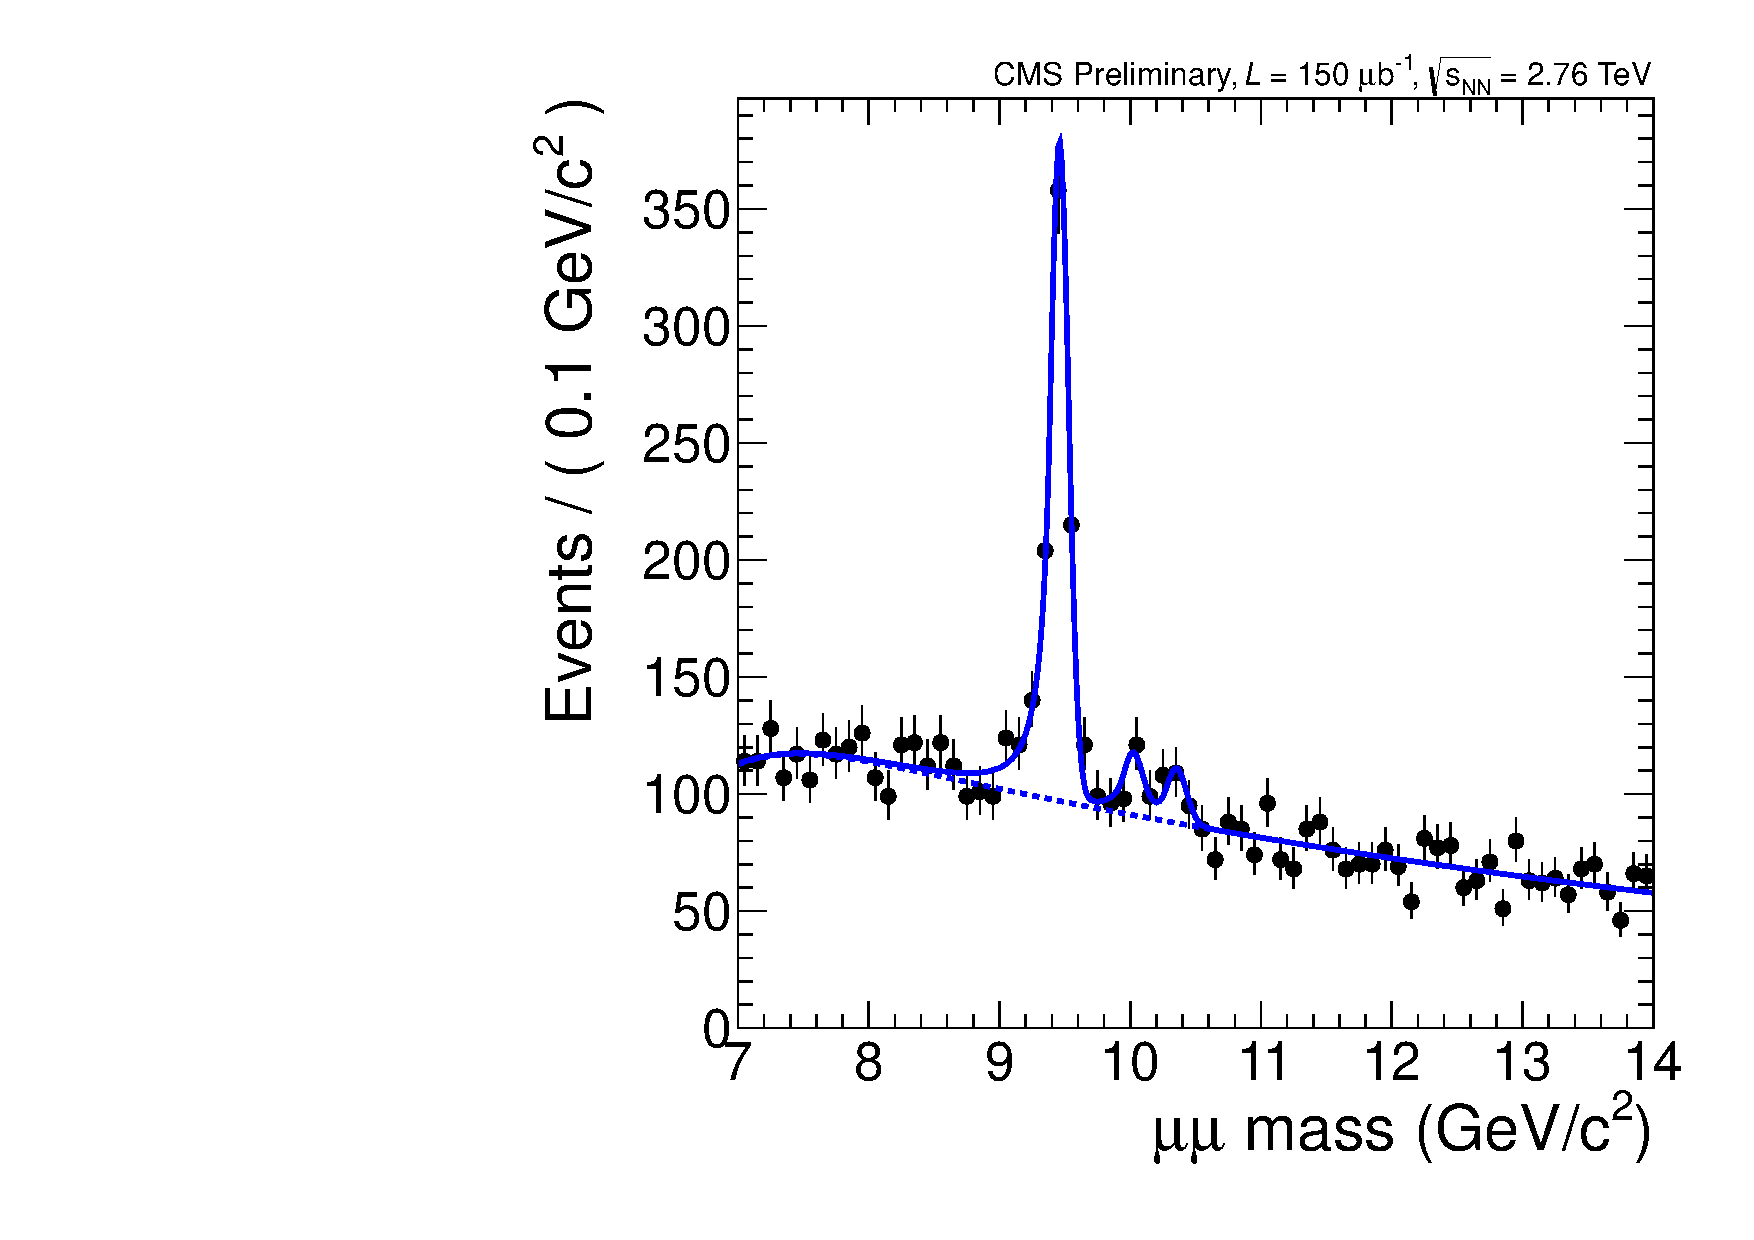
\includegraphics[angle=0,width=0.45\textwidth]{figures/pt_rapidity/hiFitPt4pt2}}
    \subfigure[\pp   data $\pt^\PgU>5\GeVc$]{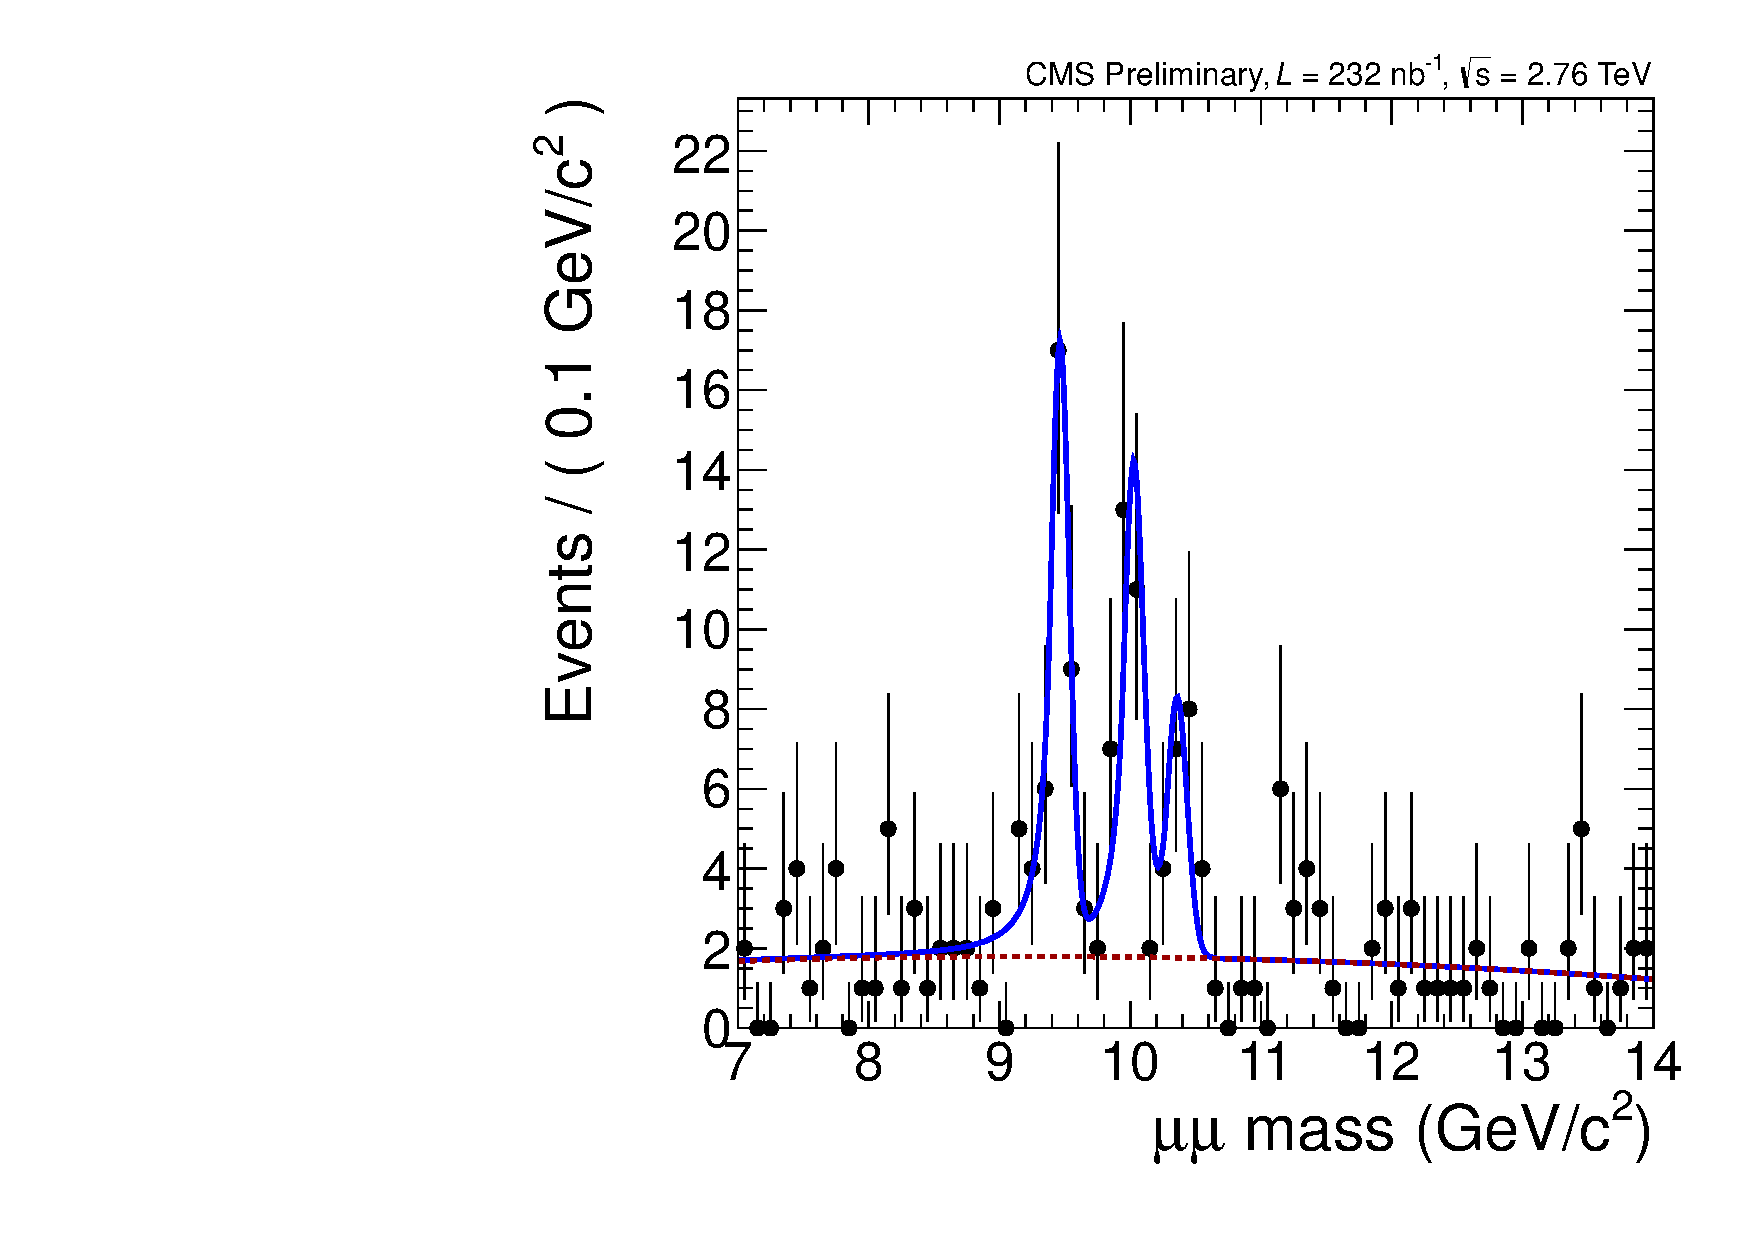
\includegraphics[angle=0,width=0.45\textwidth]{figures/pt_rapidity/ppFitPt4pt2}}
  \caption{Mass fits in ranges of dimuon momentum.}
  \label{fig:final_massfit_singlerat_rapdif}
  \end{center}
\end{figure}


\begin{figure}[hbtp]
  \begin{center}
    \subfigure[$|y|$ dependence, stat. err. only]{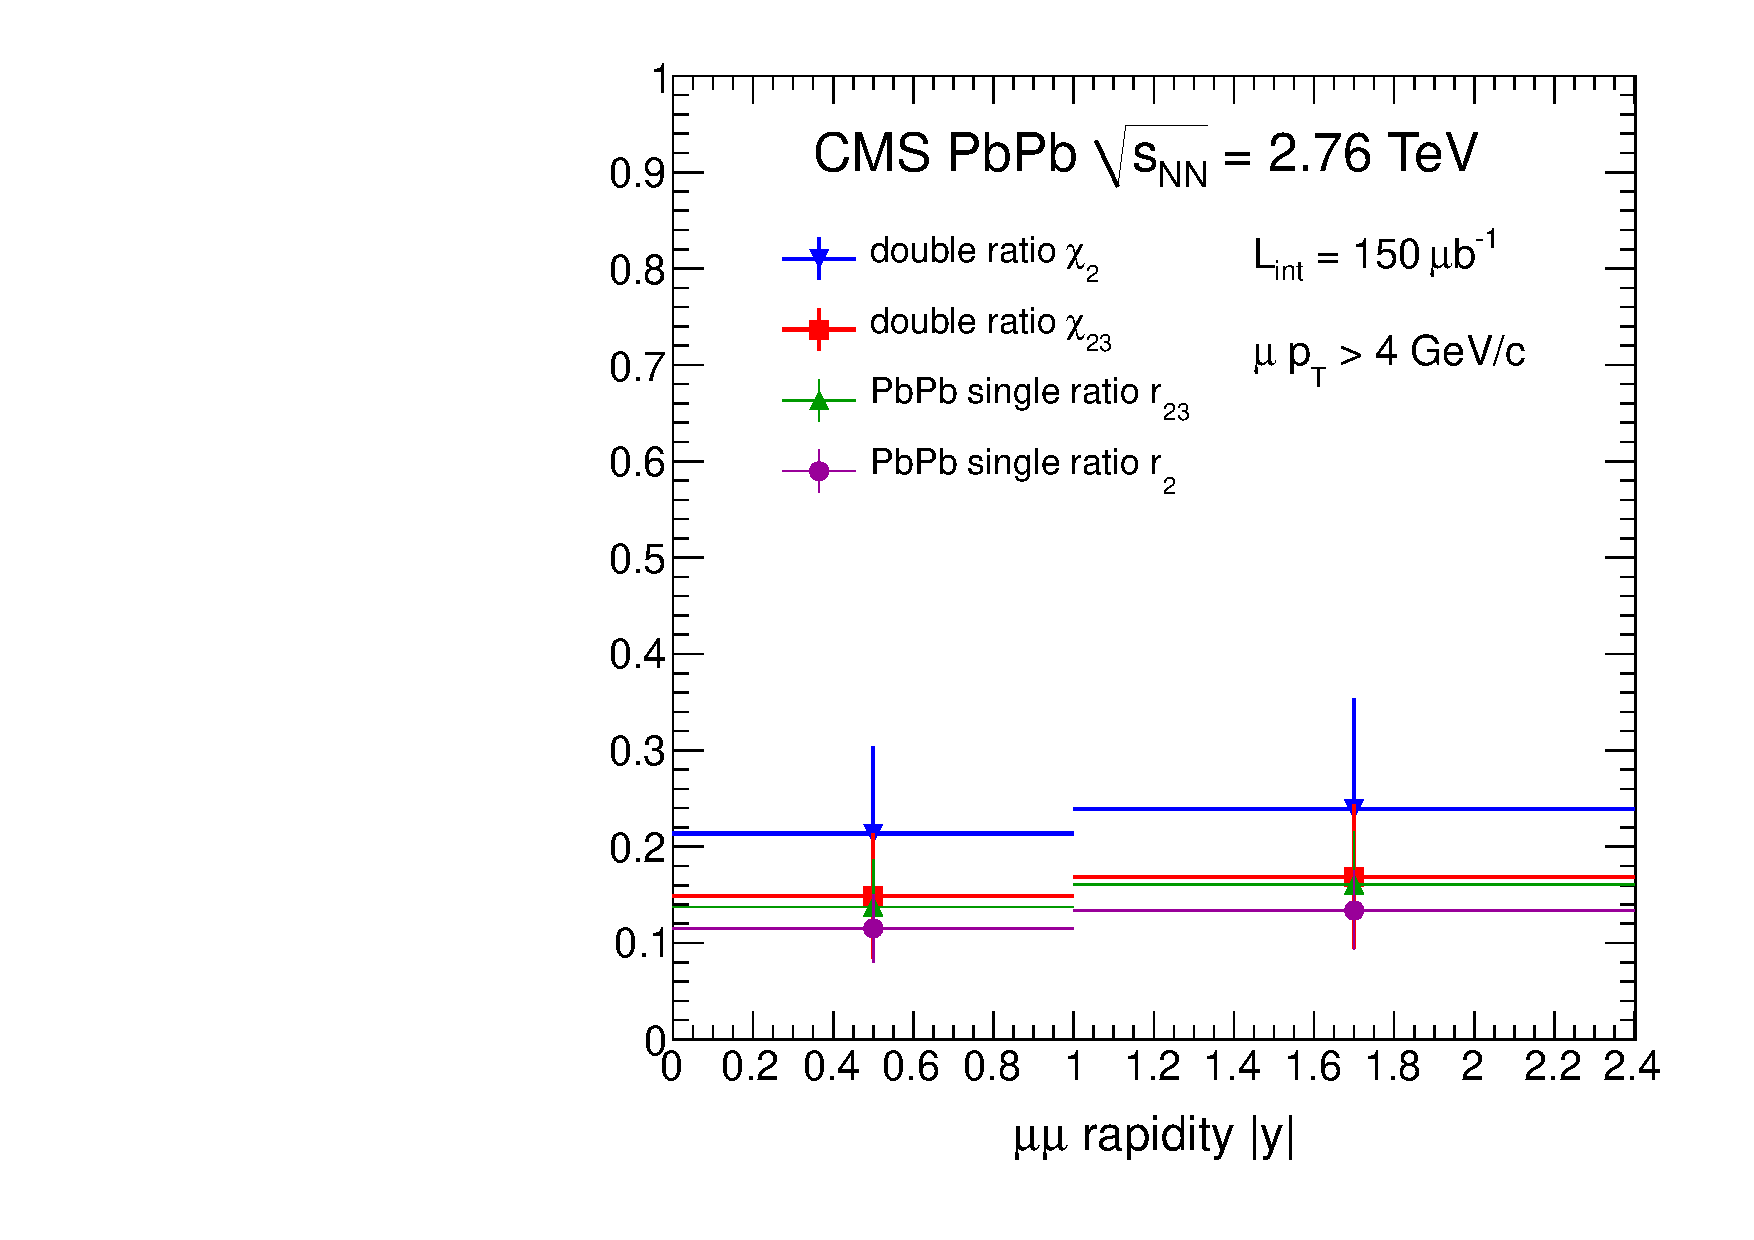
\includegraphics[angle=0,width=0.5\textwidth]{figures/pt_rapidity/RatioVsRap}}
    \subfigure[$|y|$ dependence, with syst.]{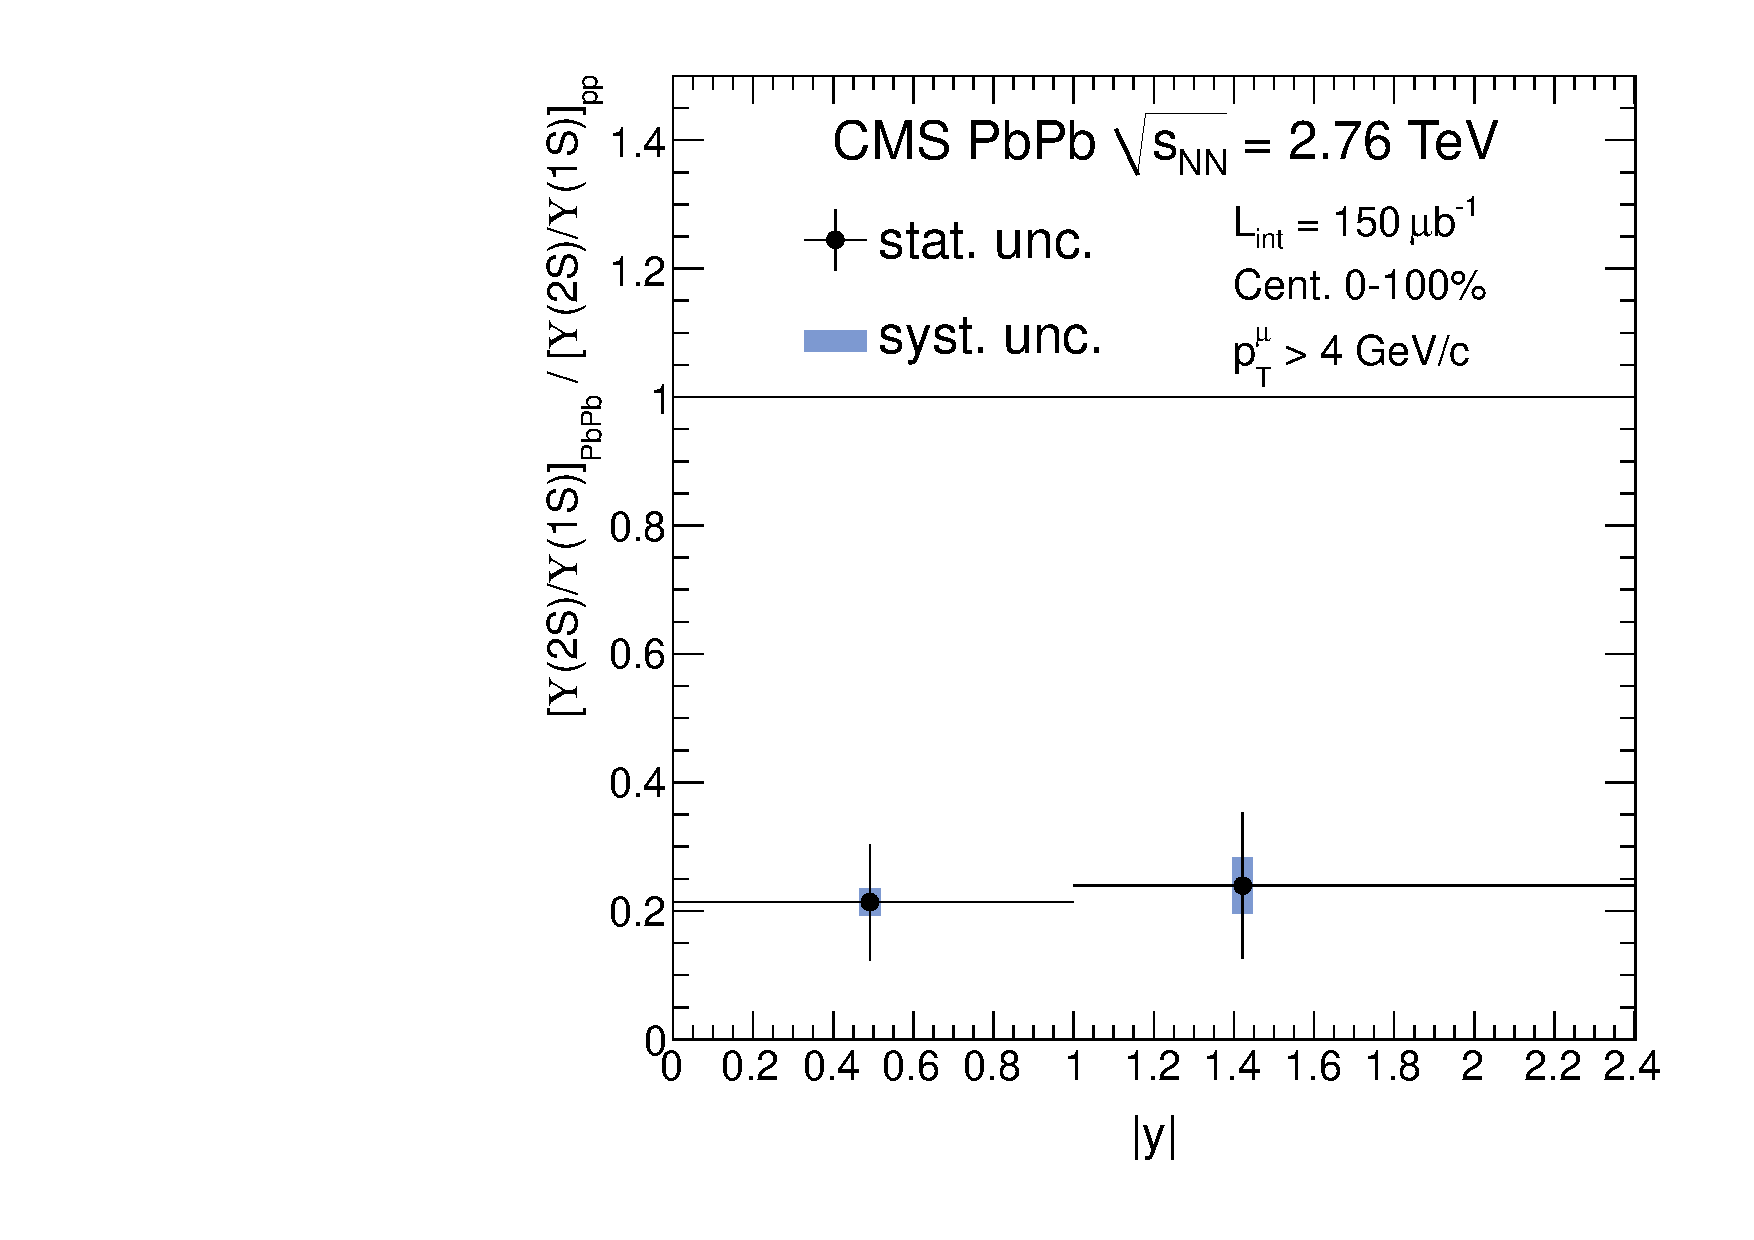
\includegraphics[angle=0,width=0.5\textwidth]{figures/pt_rapidity/RatioVsRap_x2}}  \\
	\subfigure[$\pt$ dependence, stat. err. only]{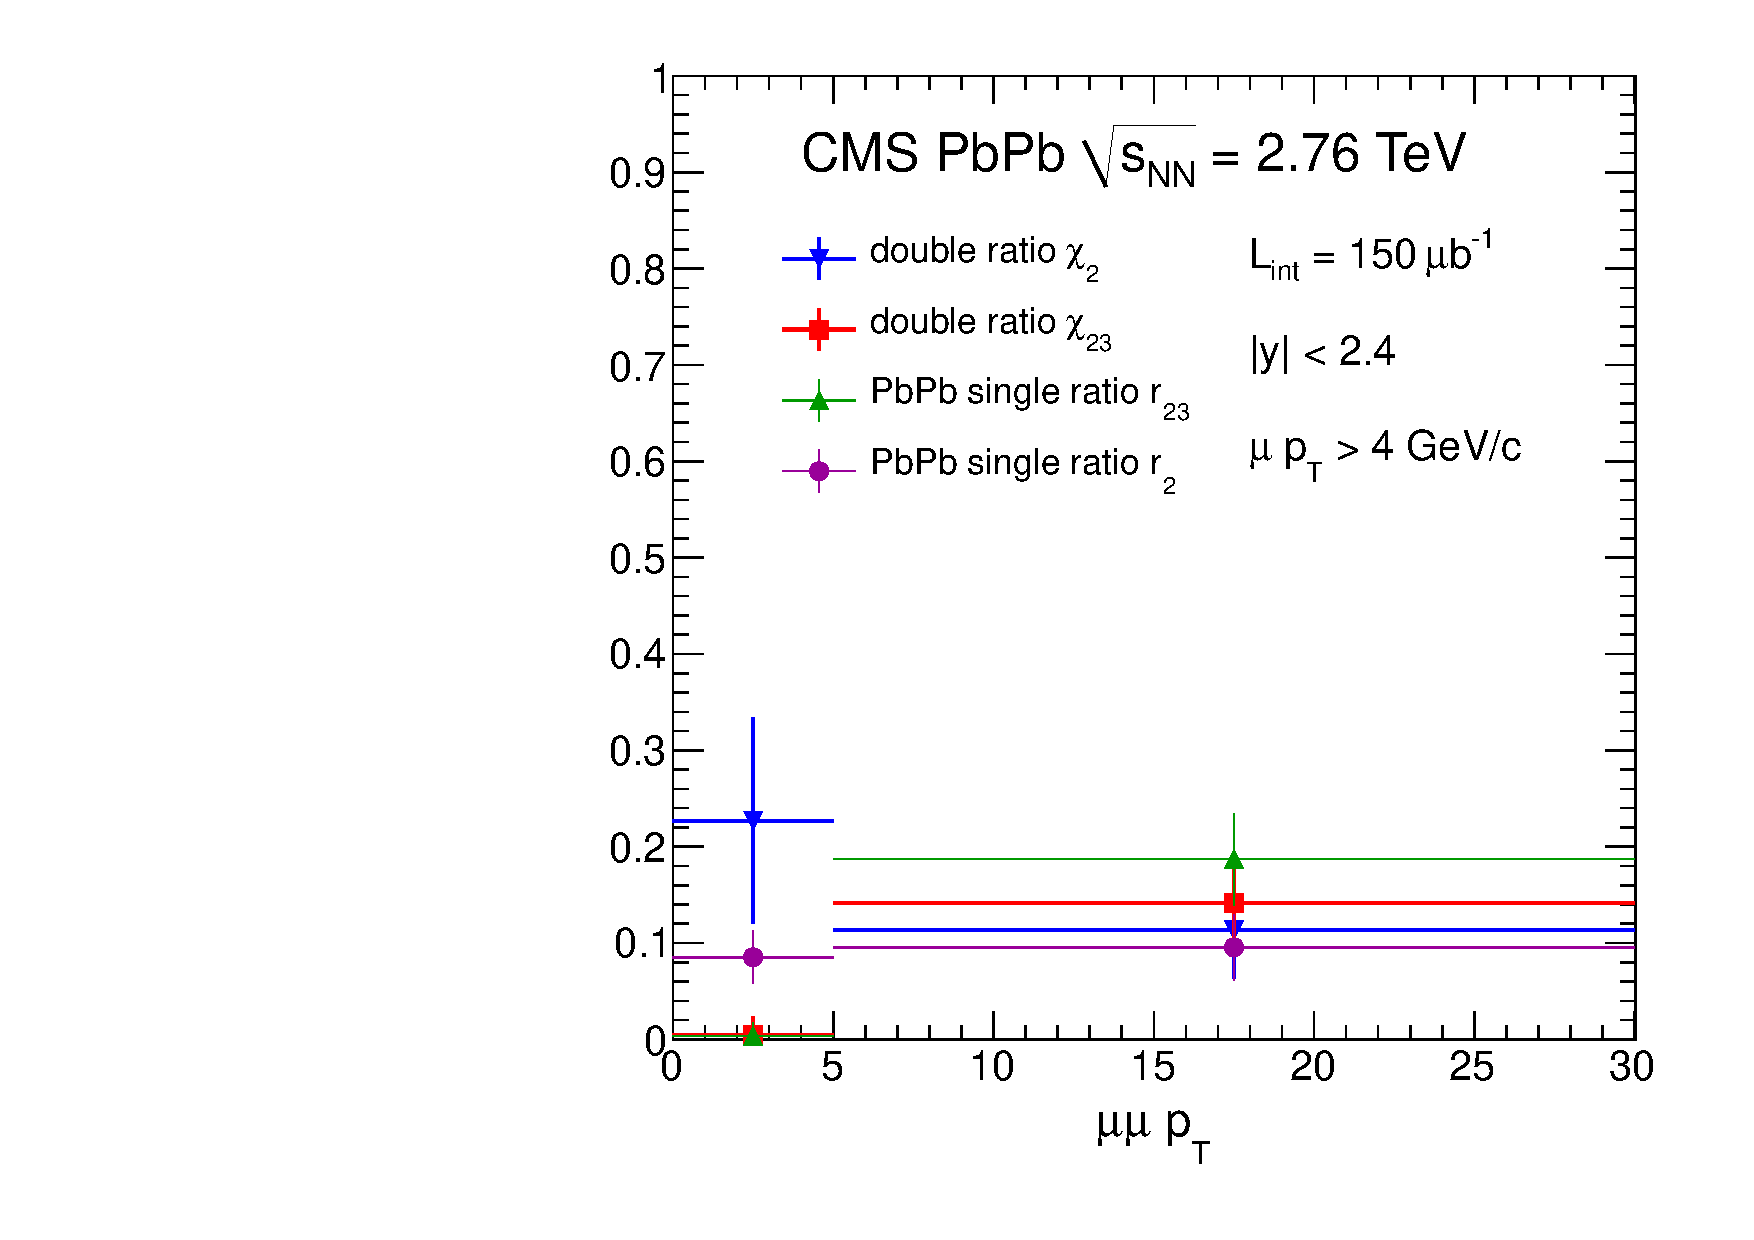
\includegraphics[angle=0,width=0.5\textwidth]{figures/pt_rapidity/RatioVsPt}}
    \subfigure[$\pt$ dependence, with syst.]{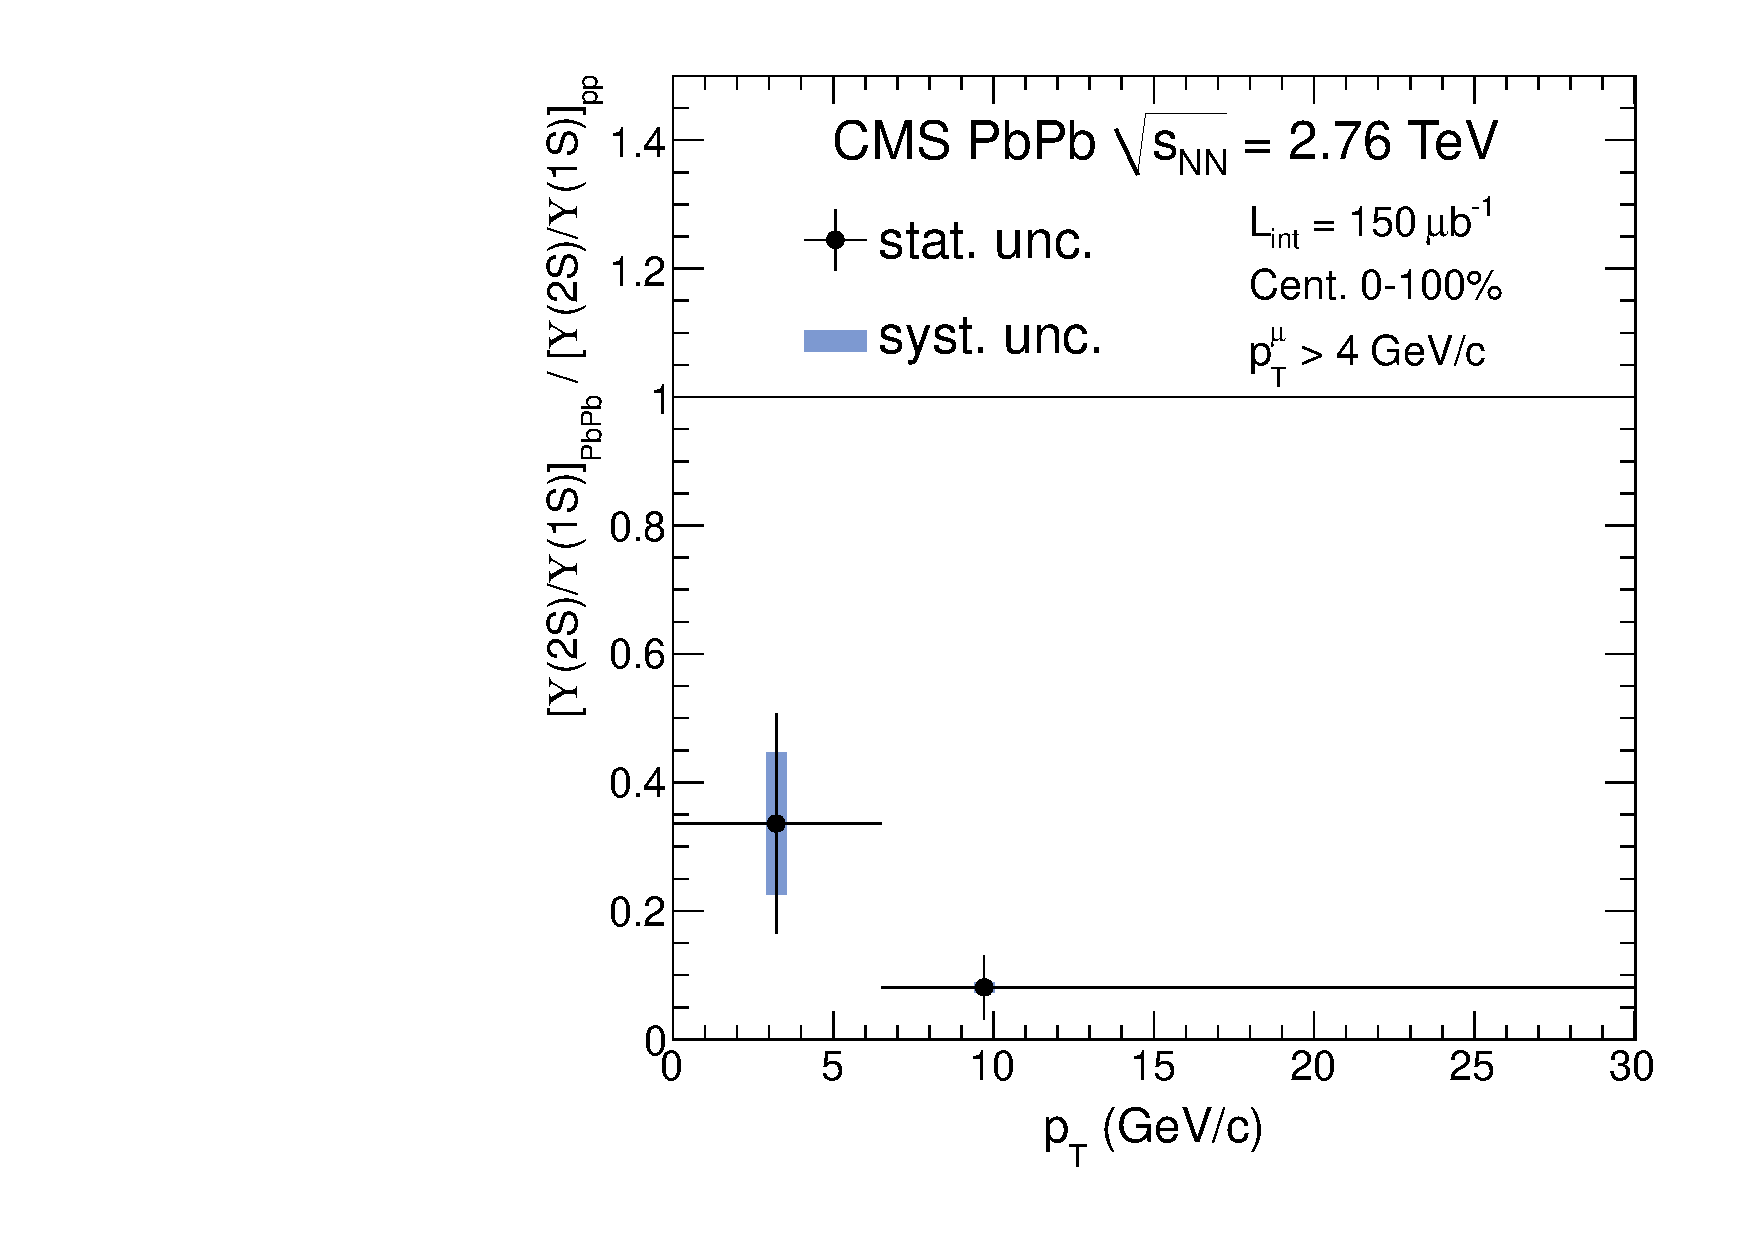
\includegraphics[angle=0,width=0.5\textwidth]{figures/pt_rapidity/RatioVsPt_x2}}
	\caption{Rapidity and \pt{} dependences of the double ratios.} 
%in PbPb and comparison with the high statistics 7TV pp results. 
  \label{fig:final_doublerat_differential}
  \end{center}
\end{figure}


\subsection{Significance} % and limits}
\label{sec:signficance}

\subsubsection{Double ratio significance}
%\subsubsection{Pseudo-experiments}

Here we attempt to quantify the significance of the observed relative
suppression of the excited-to-ground states, estimated through the
double ratios $\chi_{23}$ and $\chi_{2}$.

The nominal method employed consists of employing the profile
likelihood calculator, implemented in the Root/RooStats package ({\tt
ProfileLikelihoodCalculator}).  The null hypothesis is that
$\chi_{23}$ and $\chi_2$ are unity.  Utilizing the nominal fit
procedure, and ignoring systematic uncertainties, the obtained p-value
of our result with respect to the null hypothesis corresponds to $6.3
\sigma$.  The projections of the fit overlaid with the fit under the 
null hypothesis is shown in Fig.~\ref{fig:statSignifPlot}.

\begin{figure}
\begin{center}
\subfigure[\PbPb data fit projection]{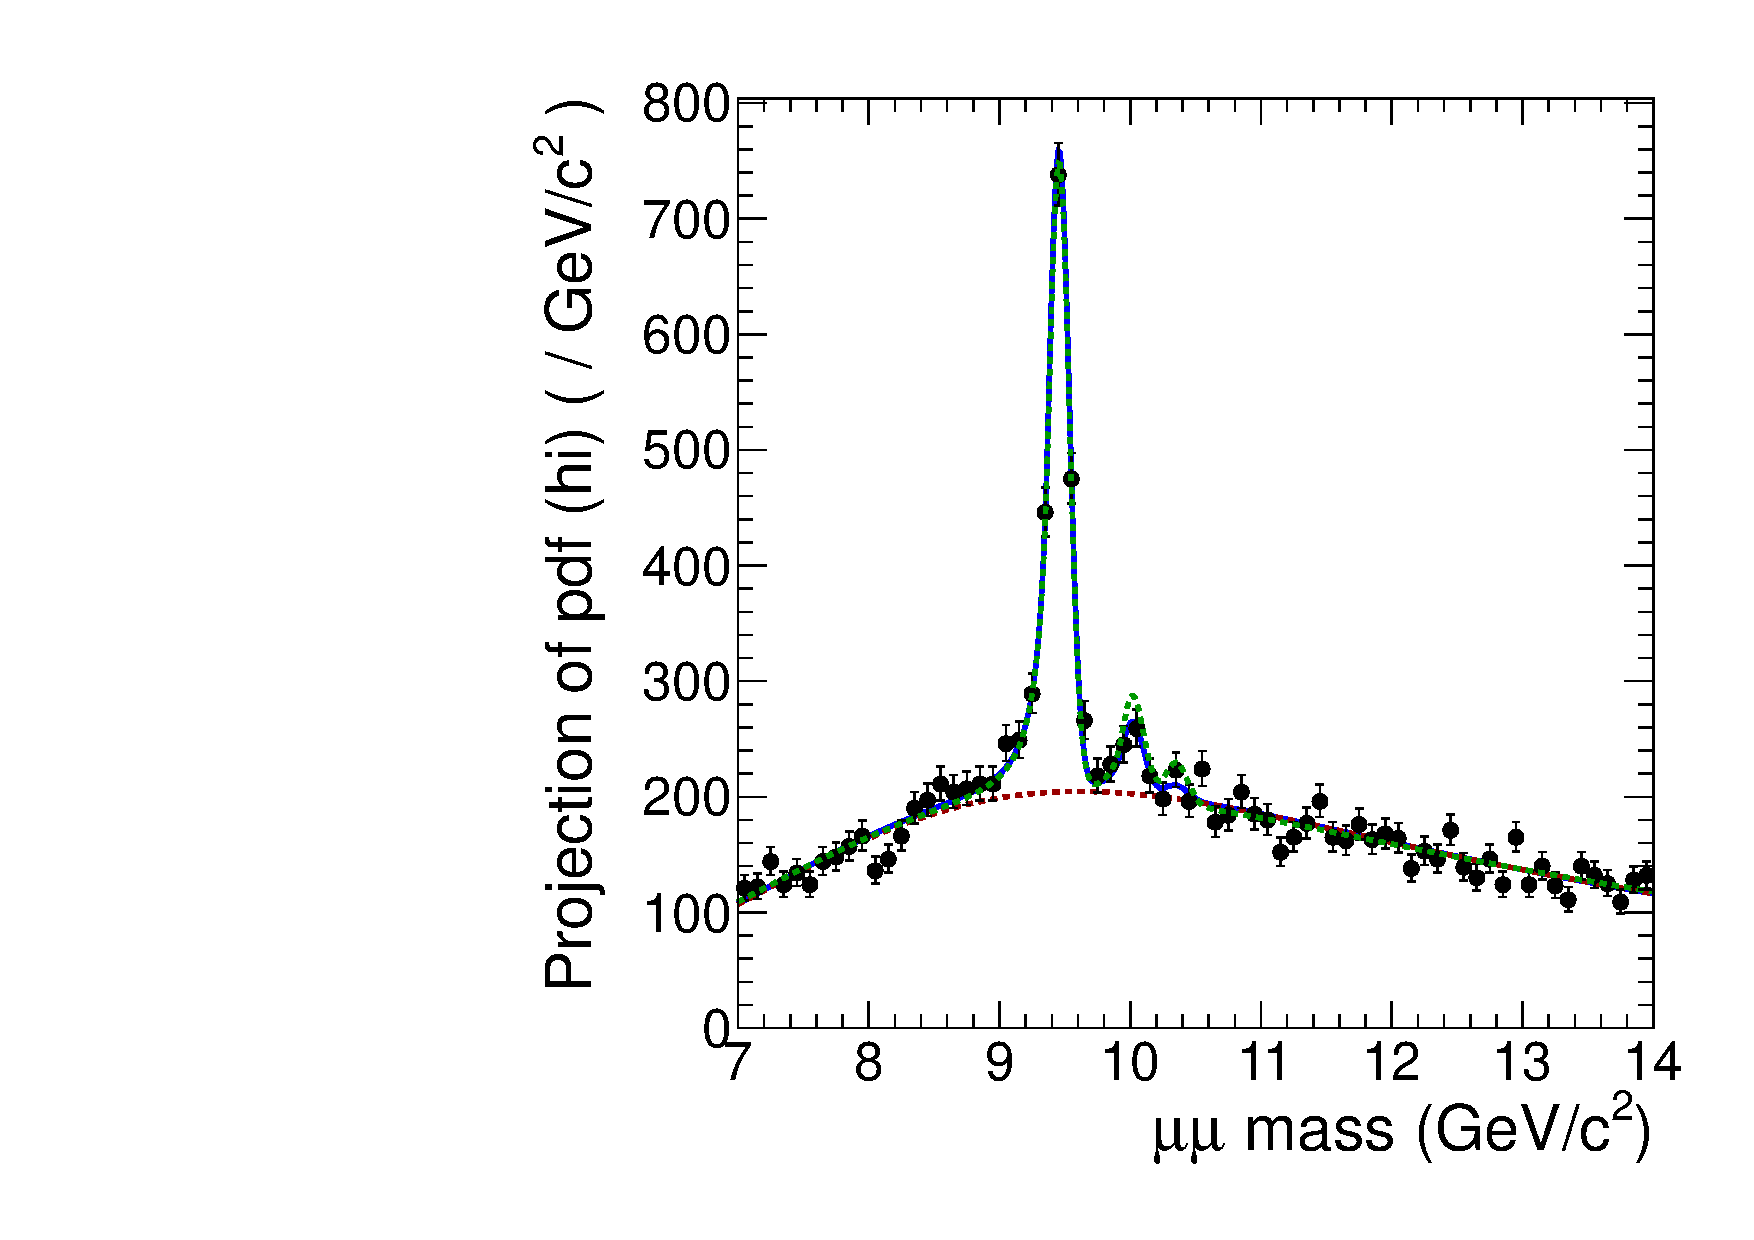
\includegraphics[width=0.45\textwidth]{figures/significance/simNull_hiFitPt40}}
\subfigure[\pp data fit projection]{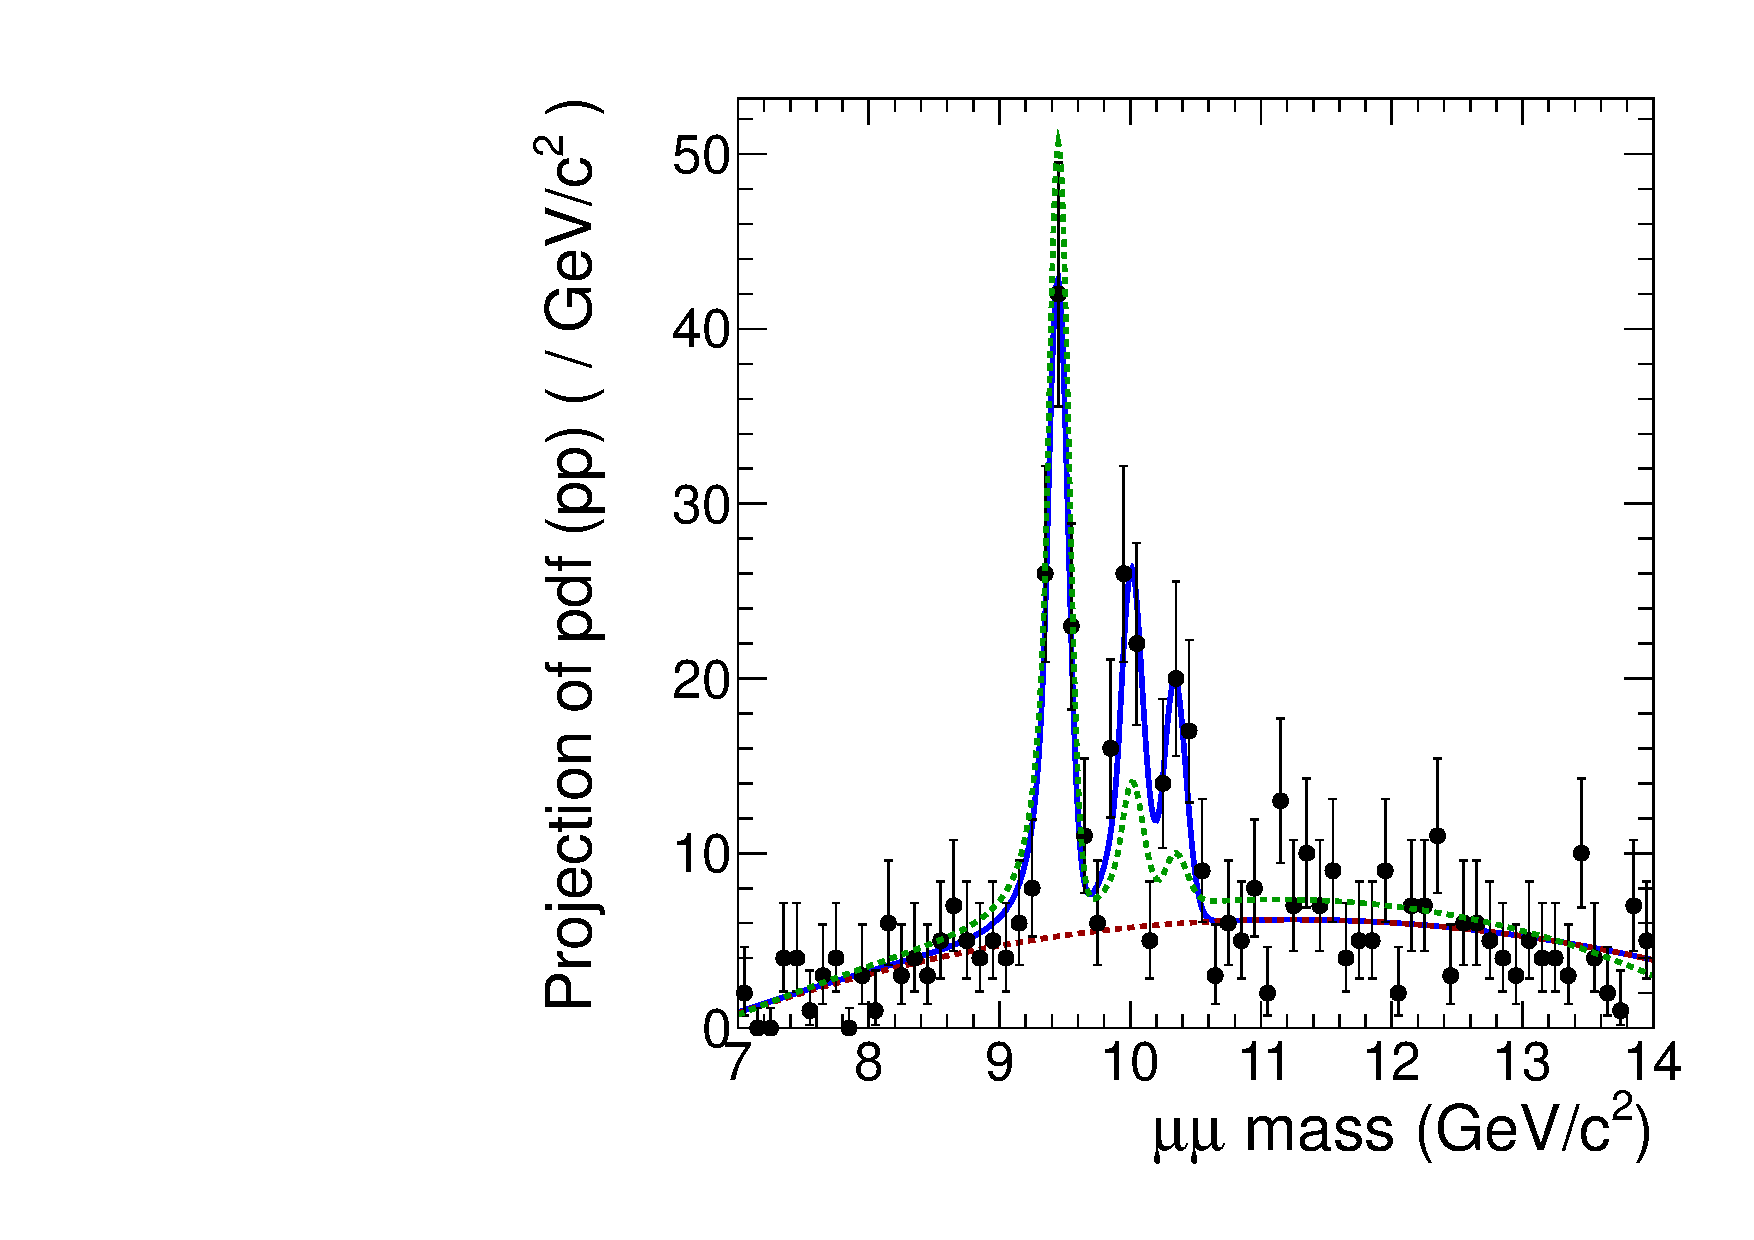
\includegraphics[width=0.45\textwidth]{figures/significance/simNull_ppFitPt40}}
\caption{Mass projections of the fit overlaid with the same fit under the assumption of the null hypothesis show in the dashed green curve, used in the estimation of the significance.}
\label{fig:statSignifPlot}
\end{center}
\end{figure}

The propagation of systematic uncertainties is challenging.  In
particular, the various systematic variations considered cannot be
readily expressed as nuisance parameters of the nominal fit model.
%
Instead, we adopt for this purpose a modified fit configuration,
identical to our nominal except that we restrict the fitting range to
$(8,14)\GeVcc$.  This has the effect of increasing the statistic fit
uncertainties on the parameters of interest (ie the double ratios) to
the level expected for the total uncertainties from the nominal fit
range, including the corresponding systematic errors.  We also include
systematic errors on the fixed FSR tail parameter.  This procedure
yields a p-value estimate corresponding to $5.4 \sigma$.  The projections
including the null hypothesis are shown in Fig.~\ref{fig:systSignifPlot}.

\begin{figure}
\begin{center}
\subfigure[\PbPb data fit projection]{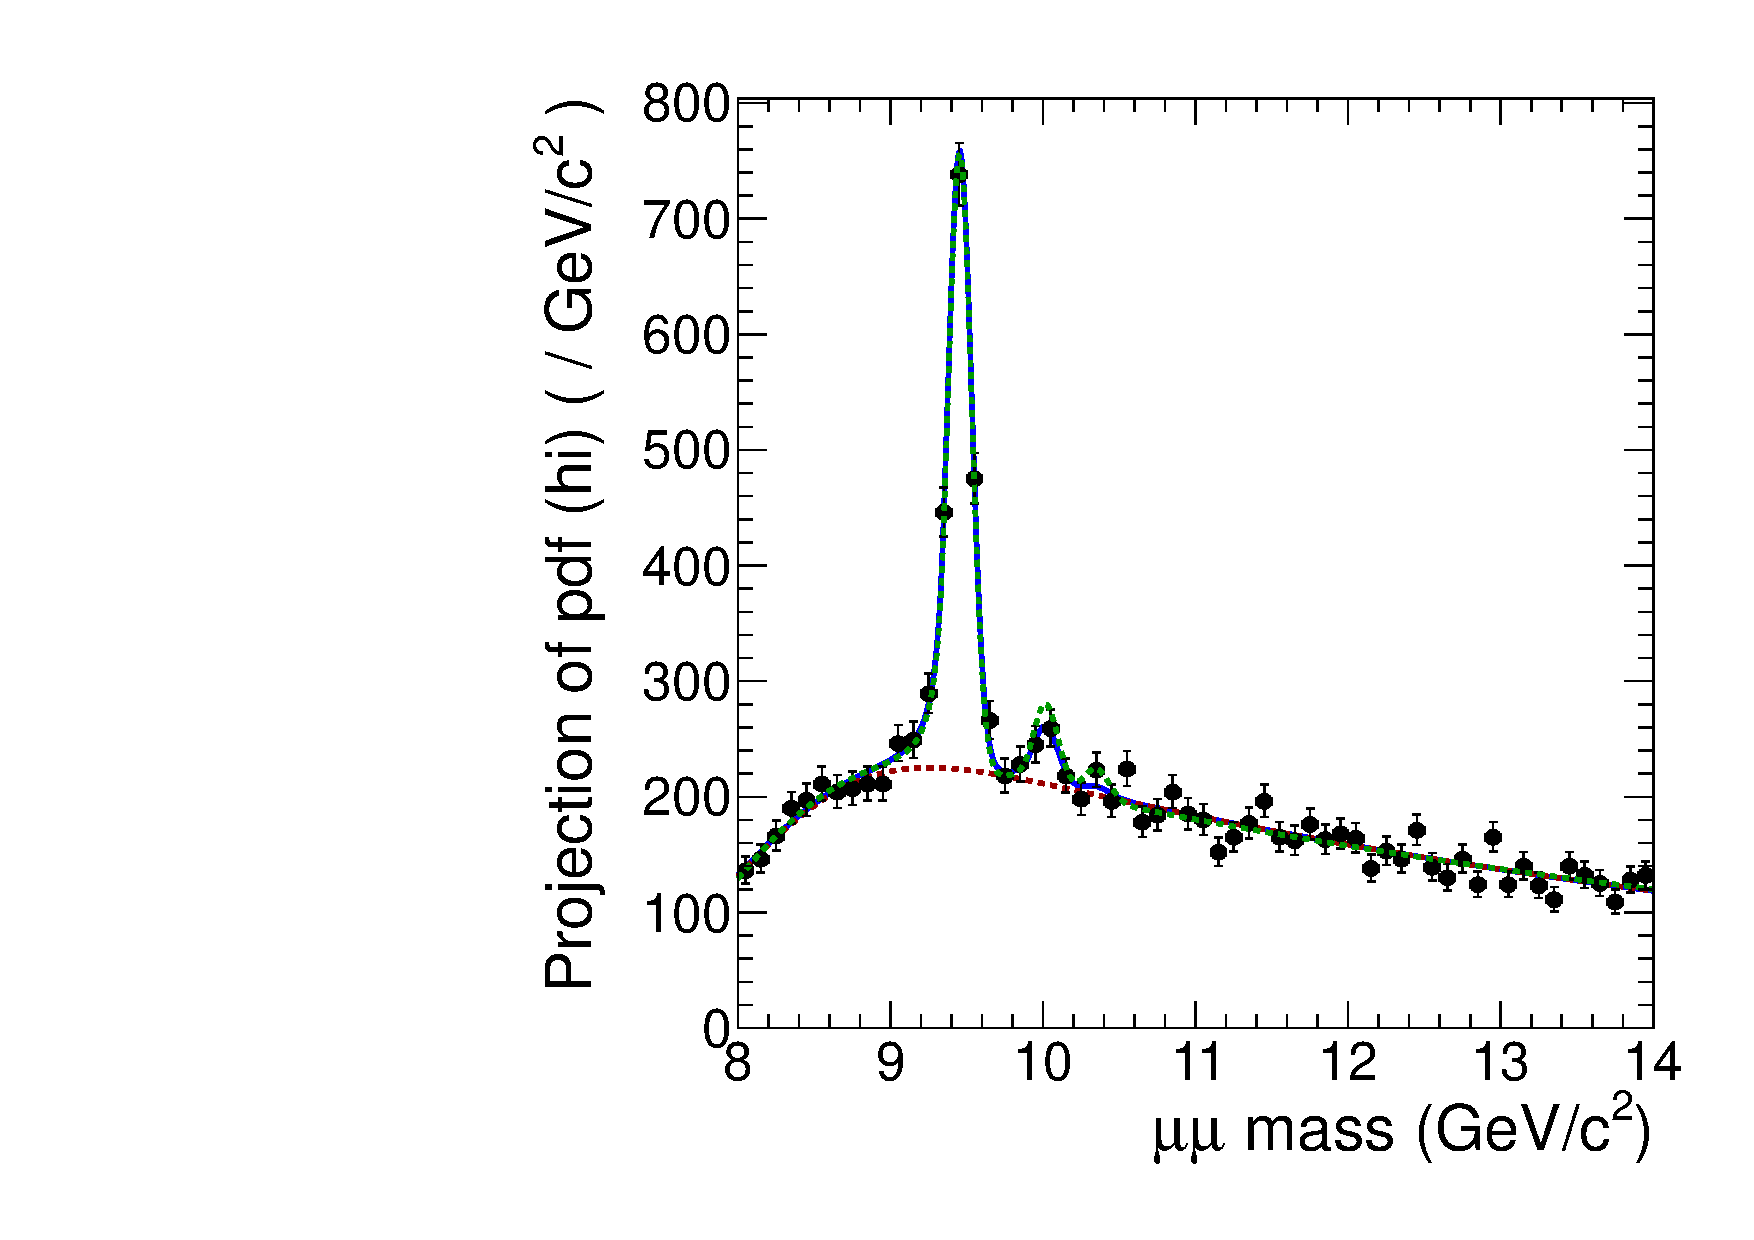
\includegraphics[width=0.45\textwidth]{figures/significance/simNullSyst_hiFitPt40}}
\subfigure[\pp data fit projection]{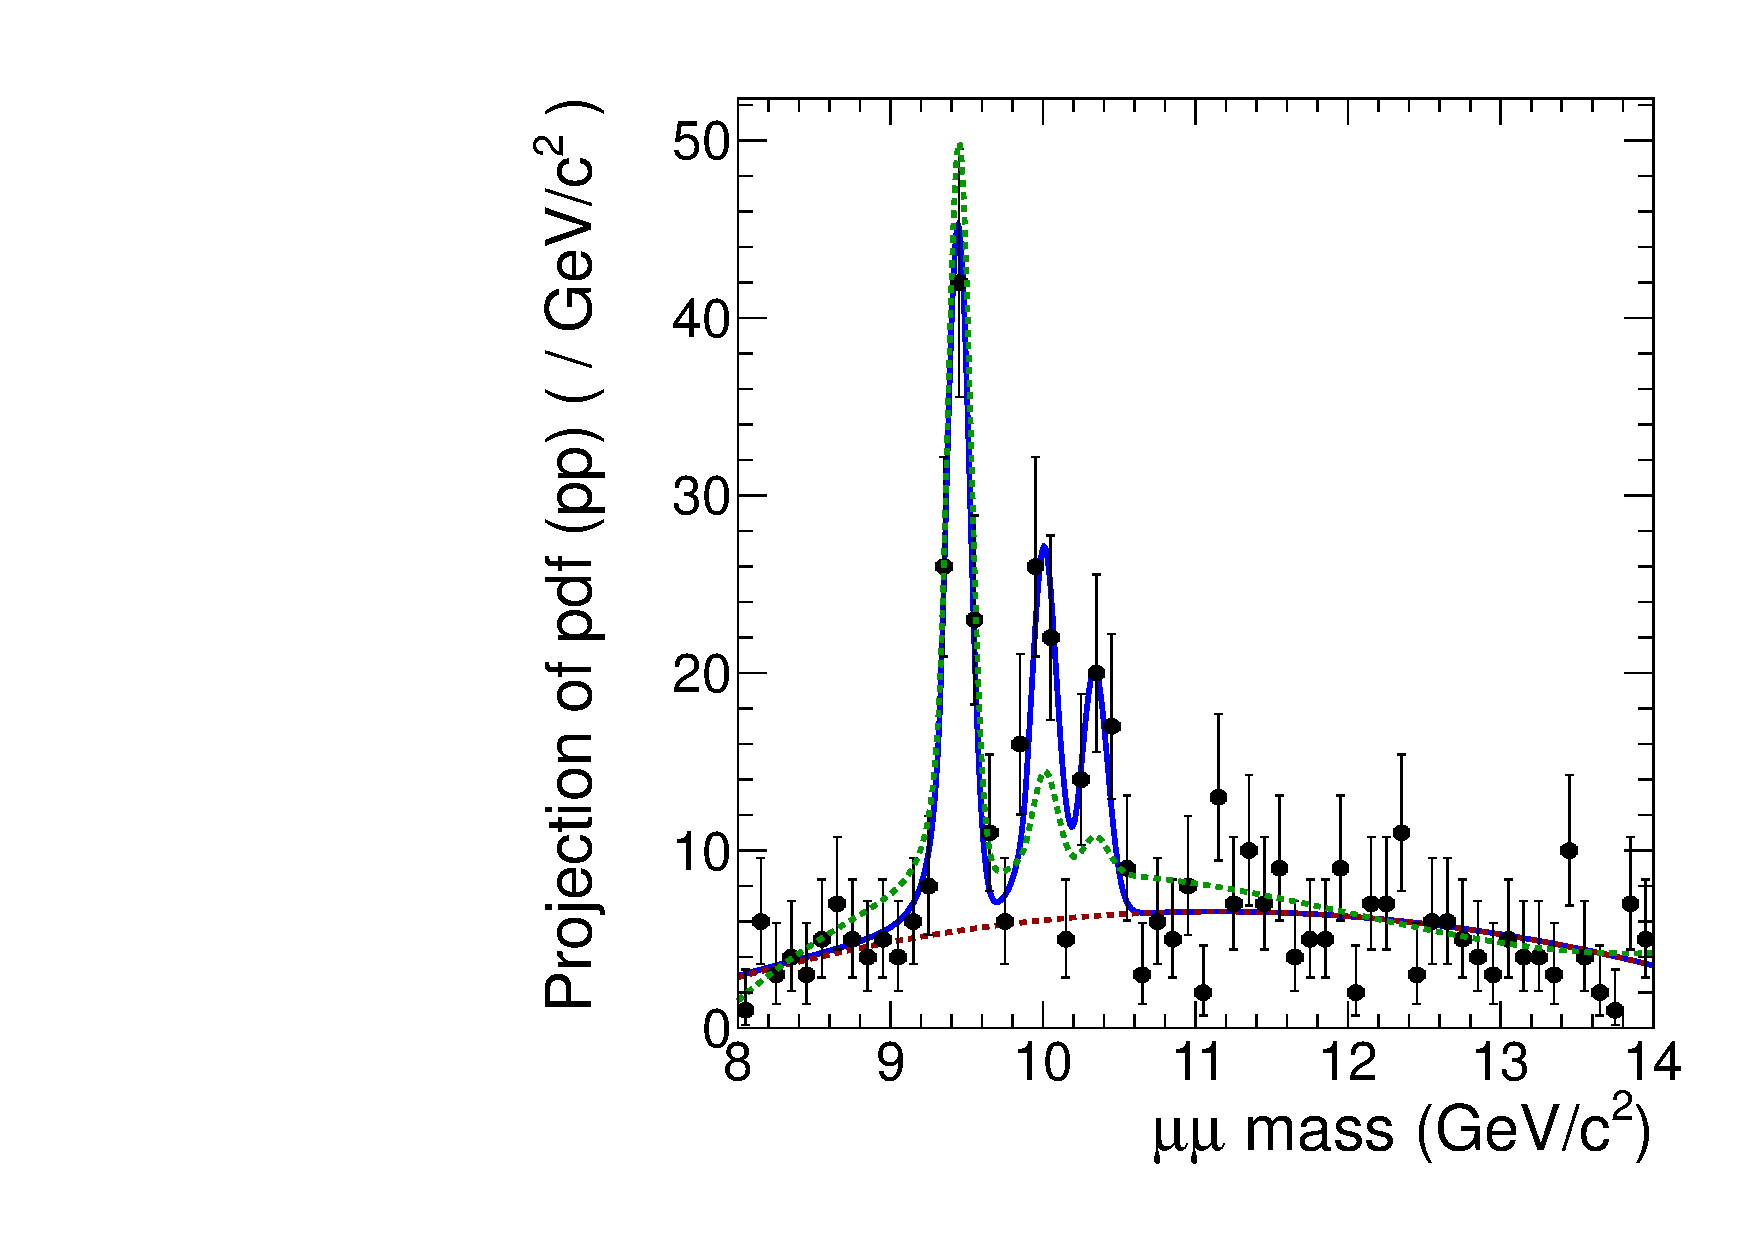
\includegraphics[width=0.45\textwidth]{figures/significance/simNullSyst_ppFitPt40}}
\caption{Mass projections of the fit overlaid with the same fit under the assumption of the null hypothesis show in the dashed green curve, used in the estimation of the significance; the fit is performed in a restricted mass range, as to account for the systematic and statistical uncertainties, as described in the text.}
\label{fig:systSignifPlot}
\end{center}
\end{figure}


%The procedure is identical to that 
For the previous measurement~\cite{prl}, we estimated the probability
for a fluctuation of the background to yield a result as extreme as
the one observed, by generating pseudo-experiments according to the
no-suppression scenario (null hypothesis), and counting the fraction
of occurrencies ($p$-value) for which the double ratio value $\chi$ is
smaller than that observed in the data.
%Specifically, the following procedure is followed:
In further detail, the following steps are performed:
%
\begin{enumerate}
\item Take the signal and background distribution for the nominal
  \Pp\Pp{} fit.  And take the background from the PbPb fit to the
  sidebands.  In the signal shape allow for known fluctuations of the
  fixed shape parameters.
\item Generate a pp pseudo-data sample using the fit to the \Pp\Pp{}
  data as a template.  In this, allow the relative contributions from
  the background and three signal resonances to shift within their
  respective statistics, but fix the total number of events to the
  number observed in data.
\item Generate background pseudo-data using the hi background model.
\item Generate the PbPb signal pseudo-data using the \Pp\Pp{} signal
  model.  The number of events is constrained so that $N_{bkg}$
  (generated in step 3) and $N_{sig}$ from this step equals the number
  of events observed in the data.  Because we are generating this with
  the \Pp\Pp{} signal model the $\chi_{23}$ is unity up to statistical
  fluctuations.
\item Fit these pseudo-data samples using the nominal fitter.
\item From the distributions of $\chi_{23}$ and $\chi_2$ obtained in
  this fashion, integrate from $-\infty$ to the observed data value to
  get the $p$-value of the measurement.
\end{enumerate}
%

To cross-check our new profiled likelihood significance calculation we
employed it on the data from the 2011 result\cite{prl}.  In this, we
calculated the significance using the procedure just described.  When
we included all systematic uncertainties we found the significance of
our result was 2.4$\,\sigma$.  Using the profile likelihood procedure
with the data and models of the 2011 measurement we find a
significance of 2.8$\,\sigma$, where this is purely statistical.  The
compatibility of these two methods provides some validation for the
profiled likelihood significance determination.

%From these distributions we find that the p value for $\chi_{23} = xxx$ to be xxx which corresponds to integrating from infinity to xxx $\sigma$ for a normal distribution.
%
\begin{figure}[hbtp]
  \begin{center}
    \subfigure[$\pt^\mu>3.5\GeVc$]{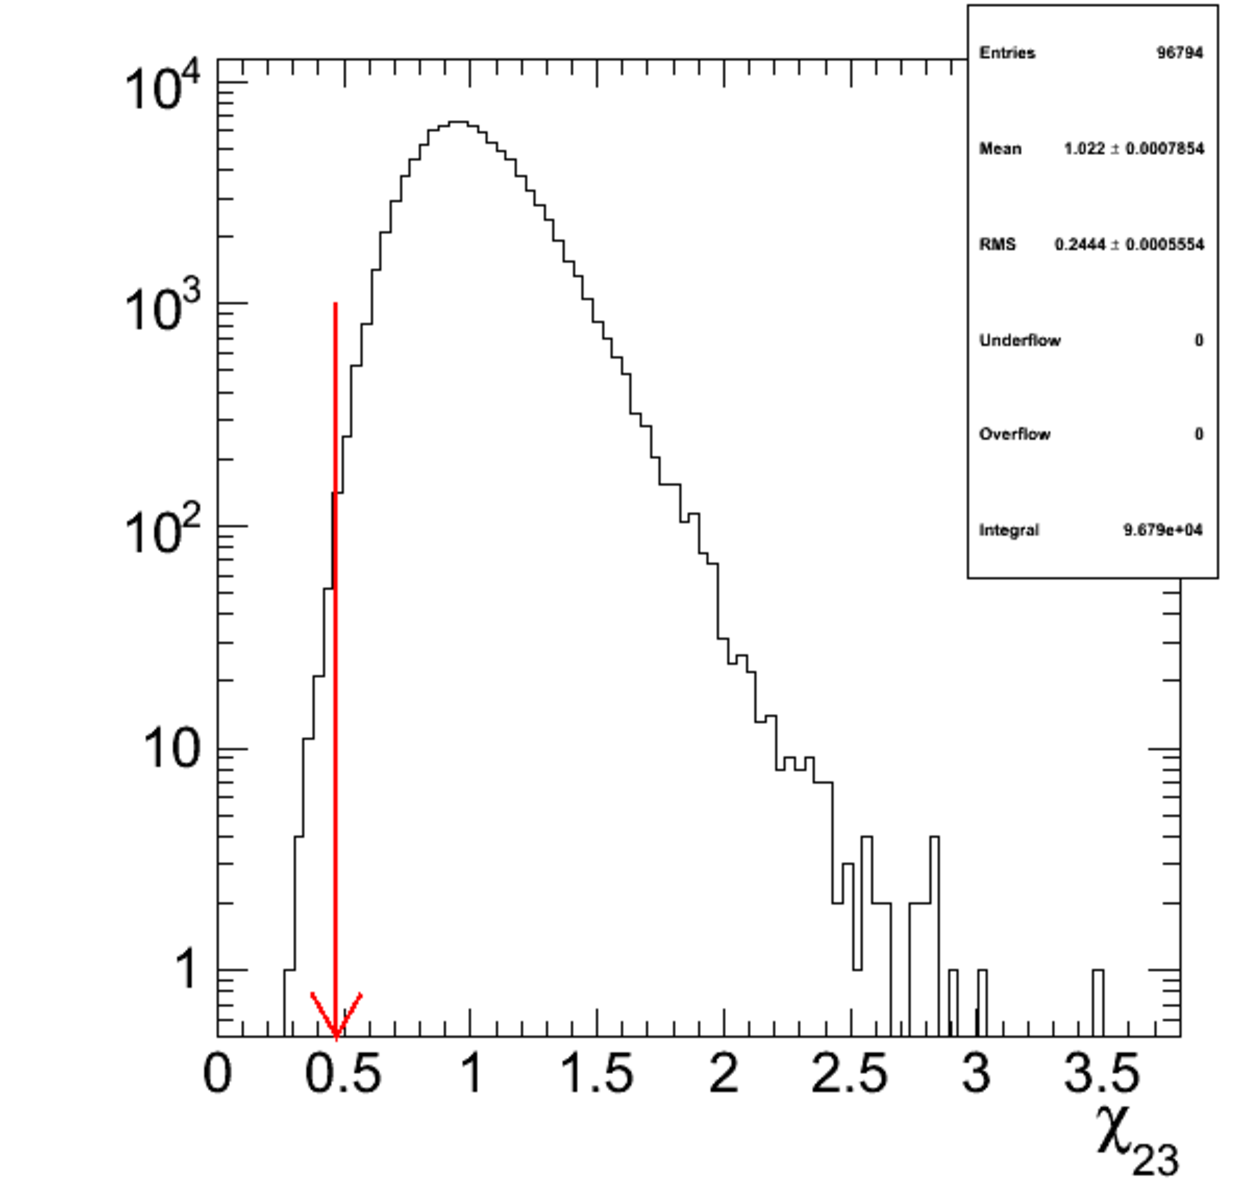
\includegraphics[angle=0,width=0.5\textwidth]{figures/significance/sensitivity35_3sigma}}
    \subfigure[$\pt^\mu>4.0\GeVc$]{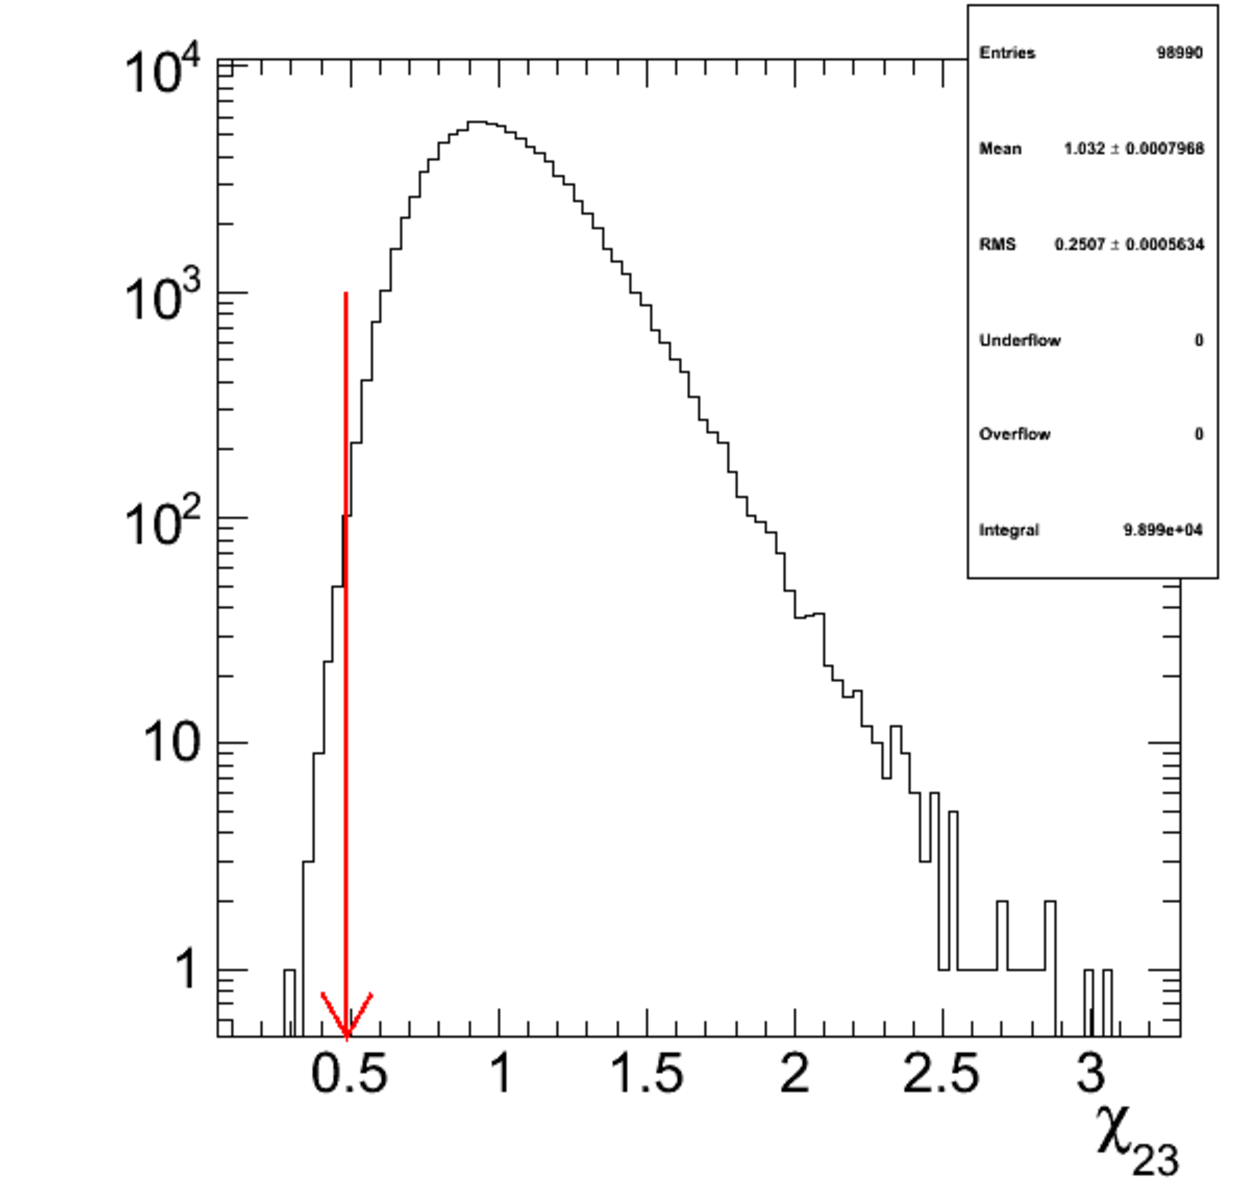
\includegraphics[angle=0,width=0.5\textwidth]{figures/significance/sensitivity40_3sigma}}
    \caption{Distributions of $\chi_{23}$ from pseudo-experiments generated under the hypothesis of no suppression.
      The arrow indicates the $\chi_{23}$ value that would correspond to $3\sigma$ significance.
}
    \label{fig:toy_nullhypo}
  \end{center}
\end{figure}

Applying this method to half of the current data and nominal fit configuration, 
the distributions of $\chi_{23}$ obtained from 10k generated pseudo-experiments are shown in~\fig{fig:toy_nullhypo}.
The vertical, red lines indicated in the plots, 
at 0.472 ($\pt^\mu>3.5\GeVc$) and 0.488 ($\pt^\mu>4.0\GeVc$), 
denote the extracted $3\,\sigma$ equivalent $\chi_{23}$ values. 
%The observed double ratio values observed in the data are smaller than these marks, 
The measured double ratio results, shown in Table~\ref{tab:final-doublerat-syst}, are indeed smaller than these marks, 
which therefore indicate a significance higher than three standard deviations. 


We then generated ~500k pseudo-experiments as per our outlined procedure ($\pt^\mu>4.0\GeVc$). The $\chi_{2}$ and $\chi_{23}$ values were smeared from unity at generation according to their respective \% systematic uncertainty.  This is an extremely conservative approach since the magnitude of the error certainly doesn't scale with the central value, but since we don't know how it scales this is what we've adopted since it is conservative.  This accounts for the systematic errors on the double ratios. As shown in \fig{fig:chi2_significance}, there are no events with an $\chi_{2}$ value as extreme as we observe.  This corresponds to a p-value smaller than 2.7e-6 which is larger than $4\,\sigma$. $4\,\sigma$ is the limit of what we can probe with this method.

\begin{figure}[hbtp]
  \begin{center}
    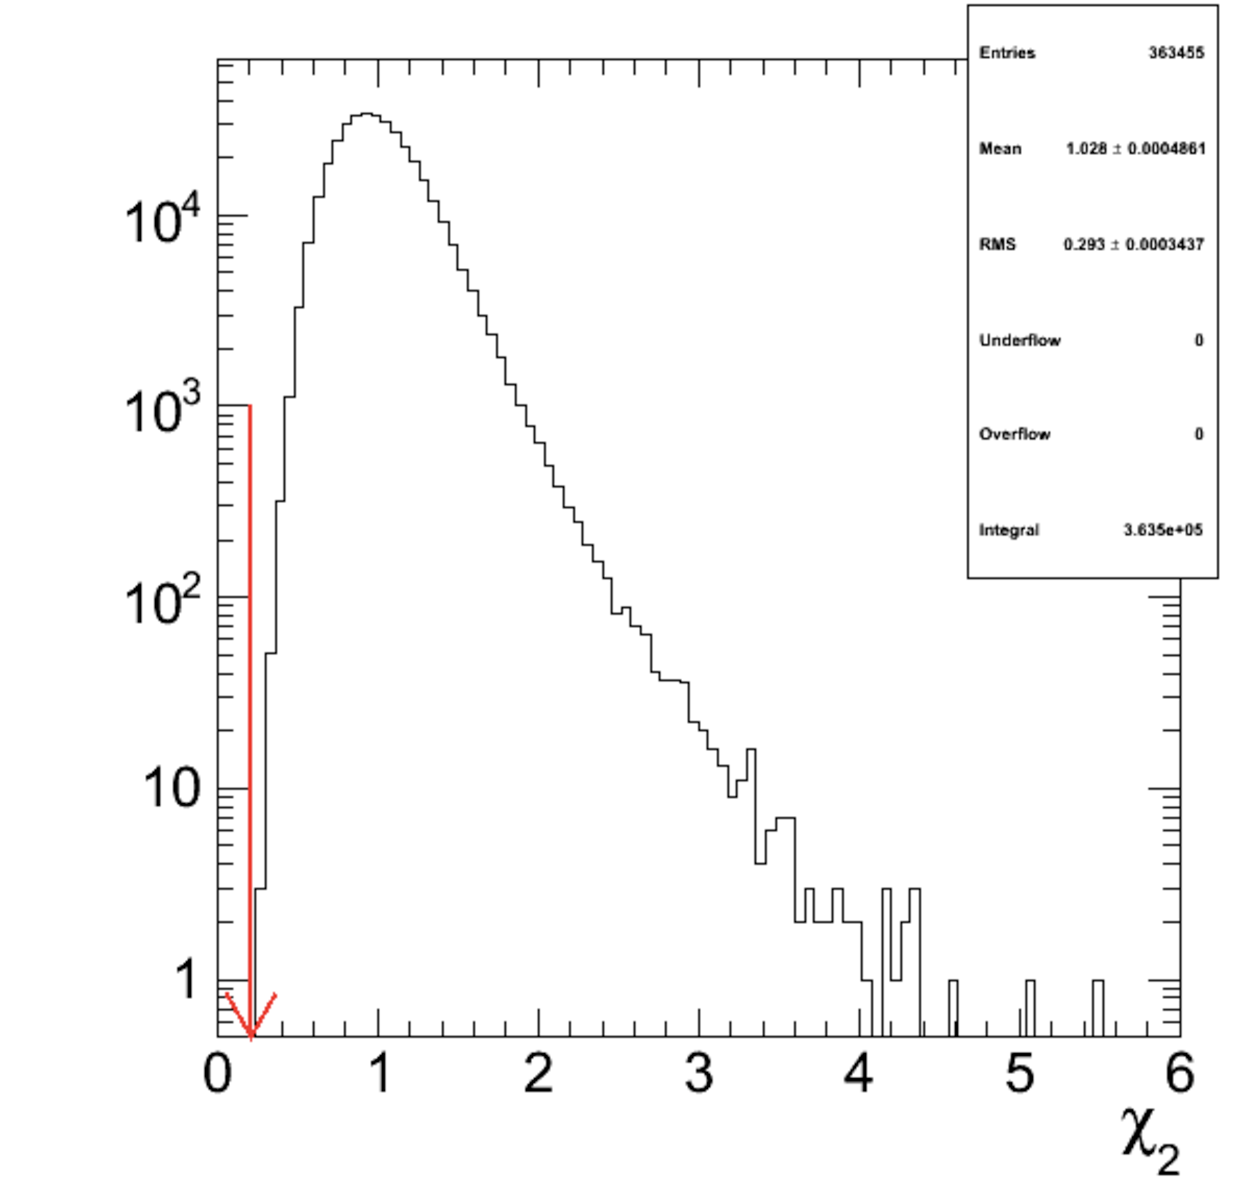
\includegraphics[angle=0,width=0.45\textwidth]{figures/significance/ToySignificance_x2.pdf}
    \caption{Distributions of $\chi_{2}$ from pseudo-experiments generated under the hypothesis of no suppression. The arrow indicates the $\chi_{2}$ value that would correspond to $4\sigma$ significance (systematic included).}
    \label{fig:chi2_significance}
  \end{center}
\end{figure}


Given the very small expected p-value, associated to the considerably higher significance of the current result compared to our previous measurement~\cite{prl}, this same method is impractical to attempt. 
Indeed, an estimation of the significance would require the tail of the $p$-value distribution in \fig{fig:toy_nullhypo} and \fig{fig:chi2_significance} to be well populated, which in turn requires larger generation of pseudo-experiments --  
%Indeed, in order to probe a p-value this small, a very high statistics pseudo-data generation would be required 
beyond what is reasonably feasible. 
This justifies the usage of the alternative method described above for estimating the significance level of our current result.



%We have estimated the p-value using only the statistical uncertainties using the profile likelihood.  This puts the p-value in the ball park of 6.5 $\sigma$.  It is completely impractical to generate pseudo-data to probe a p-value this small using that approach.  The method of estimating the systematic errors on the background shape lamentably doesn't allow us to translate them into a further statistial treatment of the p-value.  
%Another approach suggested by the statistics committee is to degrade the understanding of the background to the point that what was once a systematic uncertainty is now covered by the statistical uncertainty.  We have tried to approximate this by cutting hard on the size of the side bands, fitting only in a narrow window around the 3 resonances.  This lets leave the background much less constrained and inflates the statistial errors approriately.  In this case the p-value is between 5.5 and 6 $\sigma$.  This can only be taken as an estimate, but reinforces the statement that we pseudo-experiments are not going to soon quantify the p-value better.  Computing arbitrarily small p-values in the presence of systematic errors is in general an un-solved problem.

%
%For the meawhile, we provide an over-simplistic estimation of what might be expected: 
%For the $\pt^\mu>3.5\GeVc$ case, assuming Gaussian errors, one measures a difference $R_{23; pp} - R_{23; PbPb} =  0.553 \pm 0.117$
%For the $\pt^\mu>4.0\GeVc$ case, assuming Gaussian errors, one measures a difference $R_{23; pp} - R_{23; PbPb} =  0.553 \pm 0.117$
% assuming Gaussian errors, one computes for one of the \pt cases %(for the  $\pt^\mu>4.0\GeVc$ case) 
%a single-ratio  difference, $R_{23; pp} - R_{23; PbPb} \sim 0.739 \pm 0.164$, which stands in excess of 4.5 $\sigma$ above zero. 

%\begin{eqnarray}
%R_{23; PbPb} &=& 0.066 \pm 0.051 \\
%R_{23; pp} &=&  0.619 \pm 0.105 \\
%\Delta \equiv R_{23; pp} - R_{23; PbPb} &=& 0.553 \pm 0.117\\
%\Delta / \sigma \approx 4
%\end{eqnarray}

\subsubsection{\raa significance}
Similar approvch is applied to compute the significance for \raa. The result is summarised in Table~\ref{tab:raa_significance}. The fit plots for each case are shown in \fig{fig:raa_YnsSignif}, \fig{fig:raa_Y23sSignif}, \fig{fig:raa_Y1sSignif}, and \fig{fig:raa_Y1s0-10Signif}.

\begin{table}[!h]
  \centering
  \caption{\raa significance computed with profile likelihood ratio}
  \begin{tabular}{l|cc|c}
    \hline
     null hypo   & nominal fit -log(L) & null hypo fit -log(L) & significance \\
     \hline
     $\PgUa \raa = 1, \PgUb \raa = 1, \PgUc \raa = 1$ & -79618.2446259 & -79586.2968359 & $7.46 \sigma$ \\
     $\PgUb \raa = 1, \PgUc \raa = 1$ & -79618.2446259 & -79590.9429203 & $7.09 \sigma$ \\
     $\PgUa \raa = 1$ & -79618.2446259 & -79611.4065088 & $3.70 \sigma$ \\
     $\PgUa \raa = 1, centrality < 10\% $ & -28215.3919703 & -28204.1130248 & $4.75 \sigma$ \\
    \hline
  \end{tabular}
  \label{tab:raa_significance}
\end{table}


\begin{figure}
\begin{center}
\subfigure[\PbPb data fit projection]{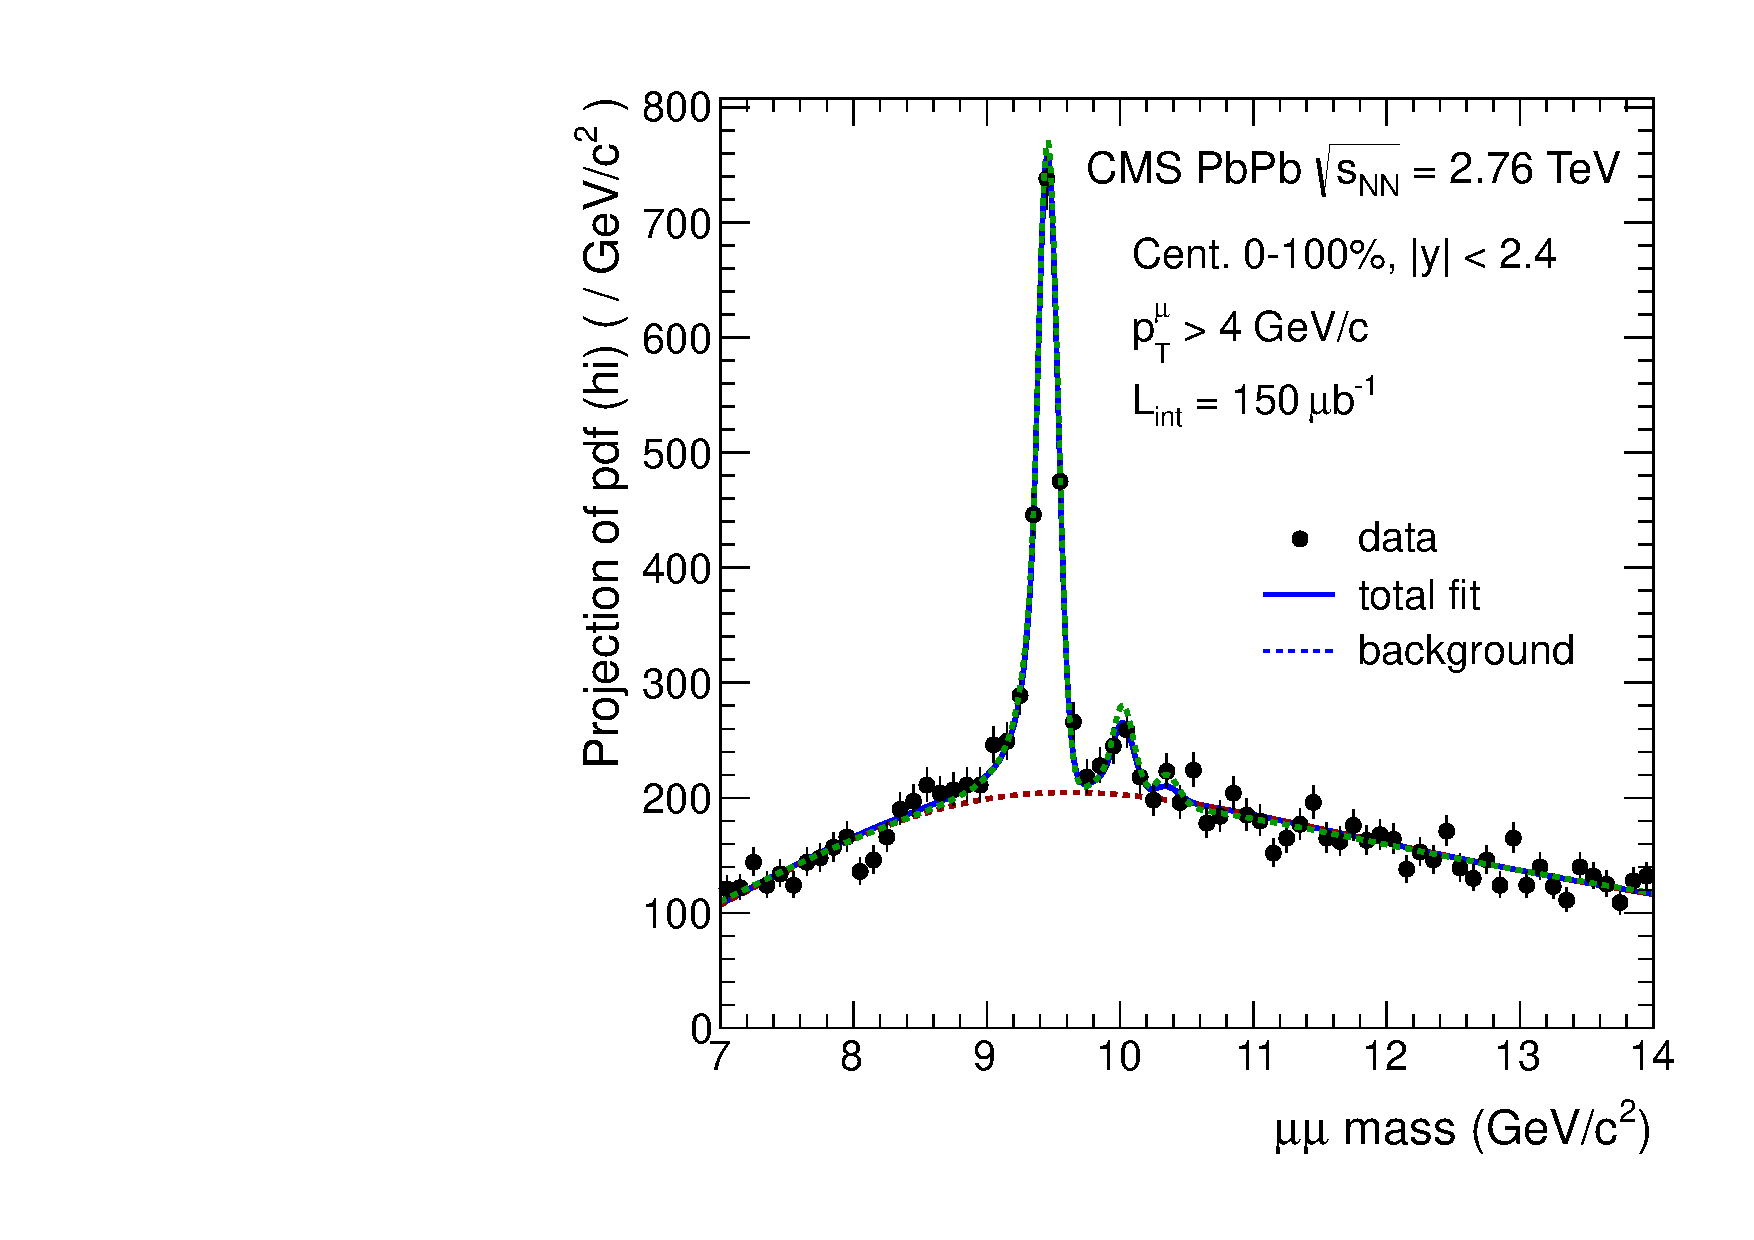
\includegraphics[width=0.45\textwidth]{figures/significance/hiFitYnSsignificance.pdf}}
\subfigure[\pp data fit projection]{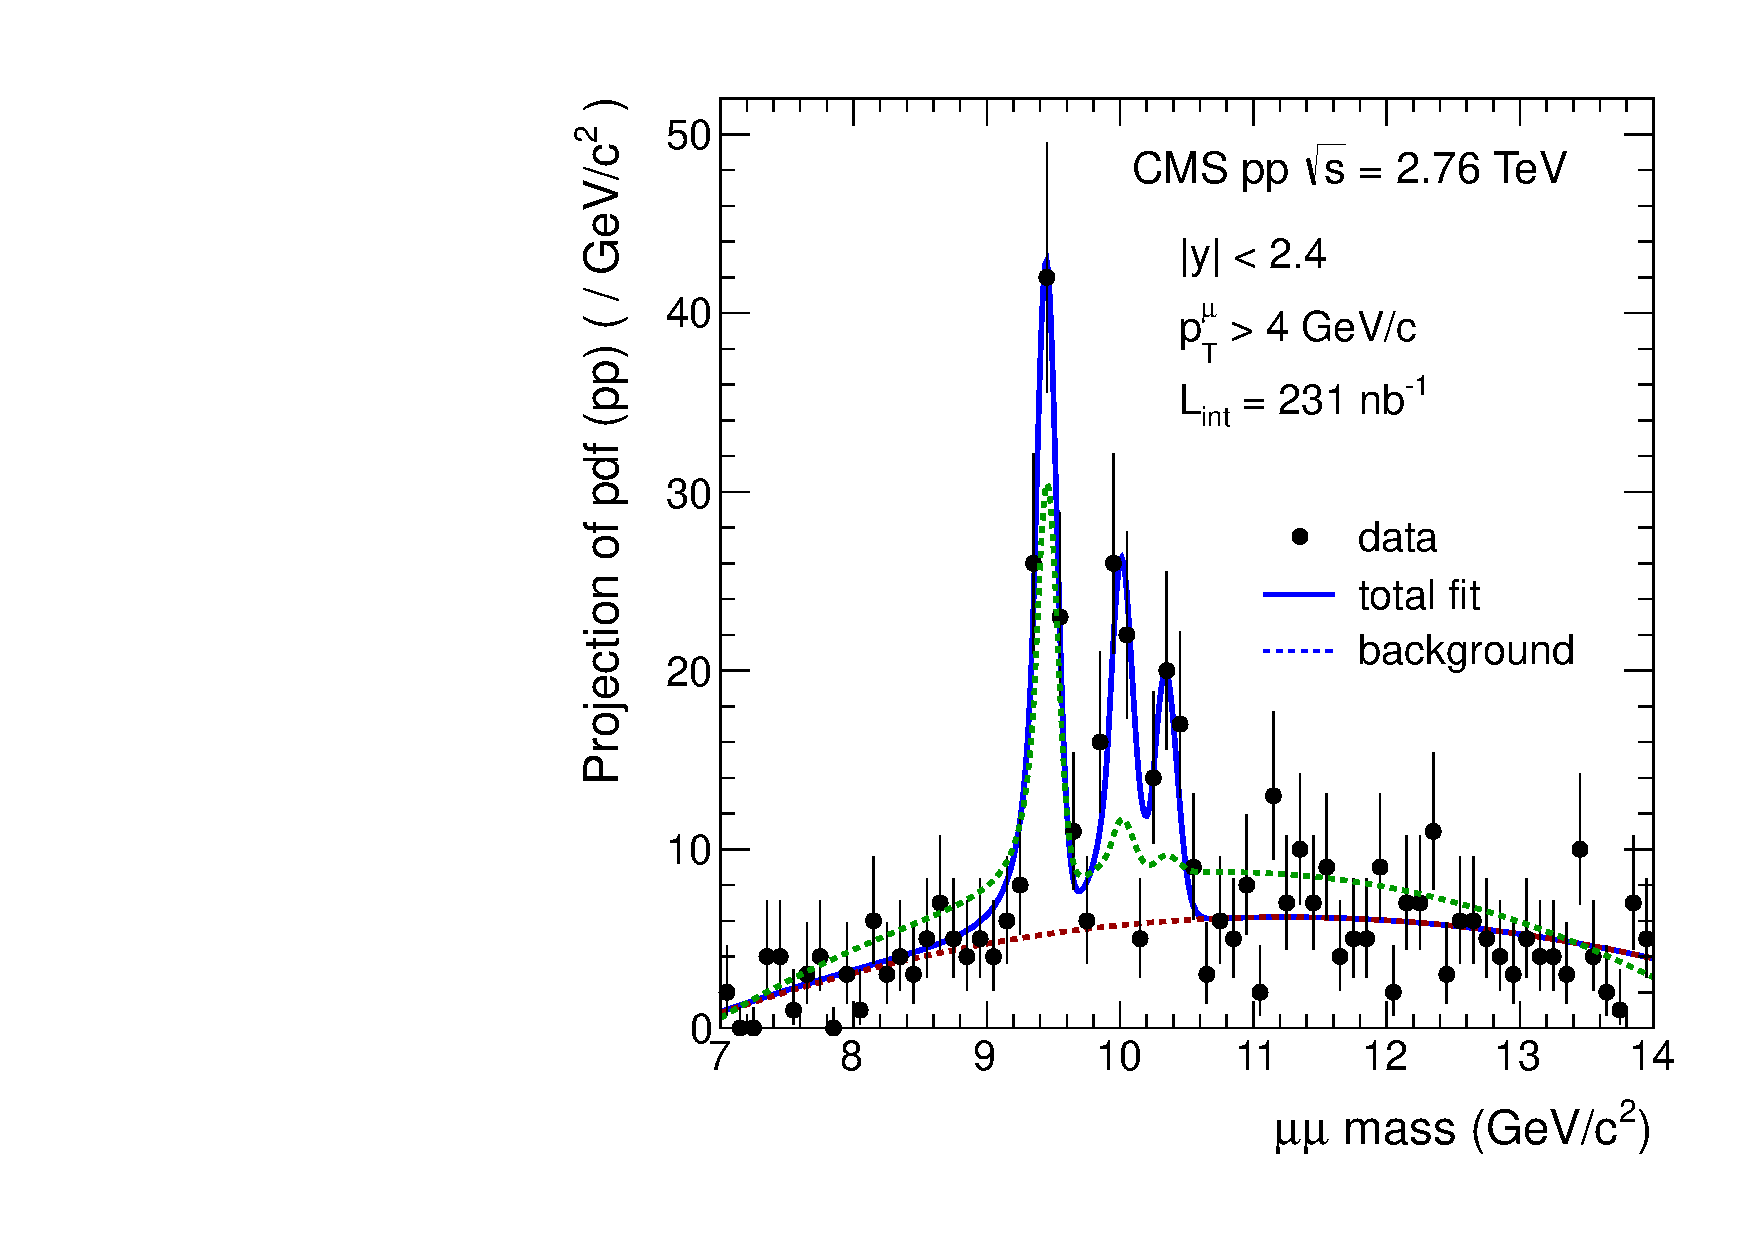
\includegraphics[width=0.45\textwidth]{figures/significance/ppFitYnSsignificance.pdf}}
\caption{Mass projections of the fit overlaid with the same fit under the assumption of the null hypothesis show in the dashed green curve, used in the estimation of the significance. Null hypothesis: $\PgUa \raa = 1, \PgUb \raa = 1, \PgUc \raa = 1$ }
\label{fig:raa_YnsSignif}
\end{center}
\end{figure}

\begin{figure}
\begin{center}
\subfigure[\PbPb data fit projection]{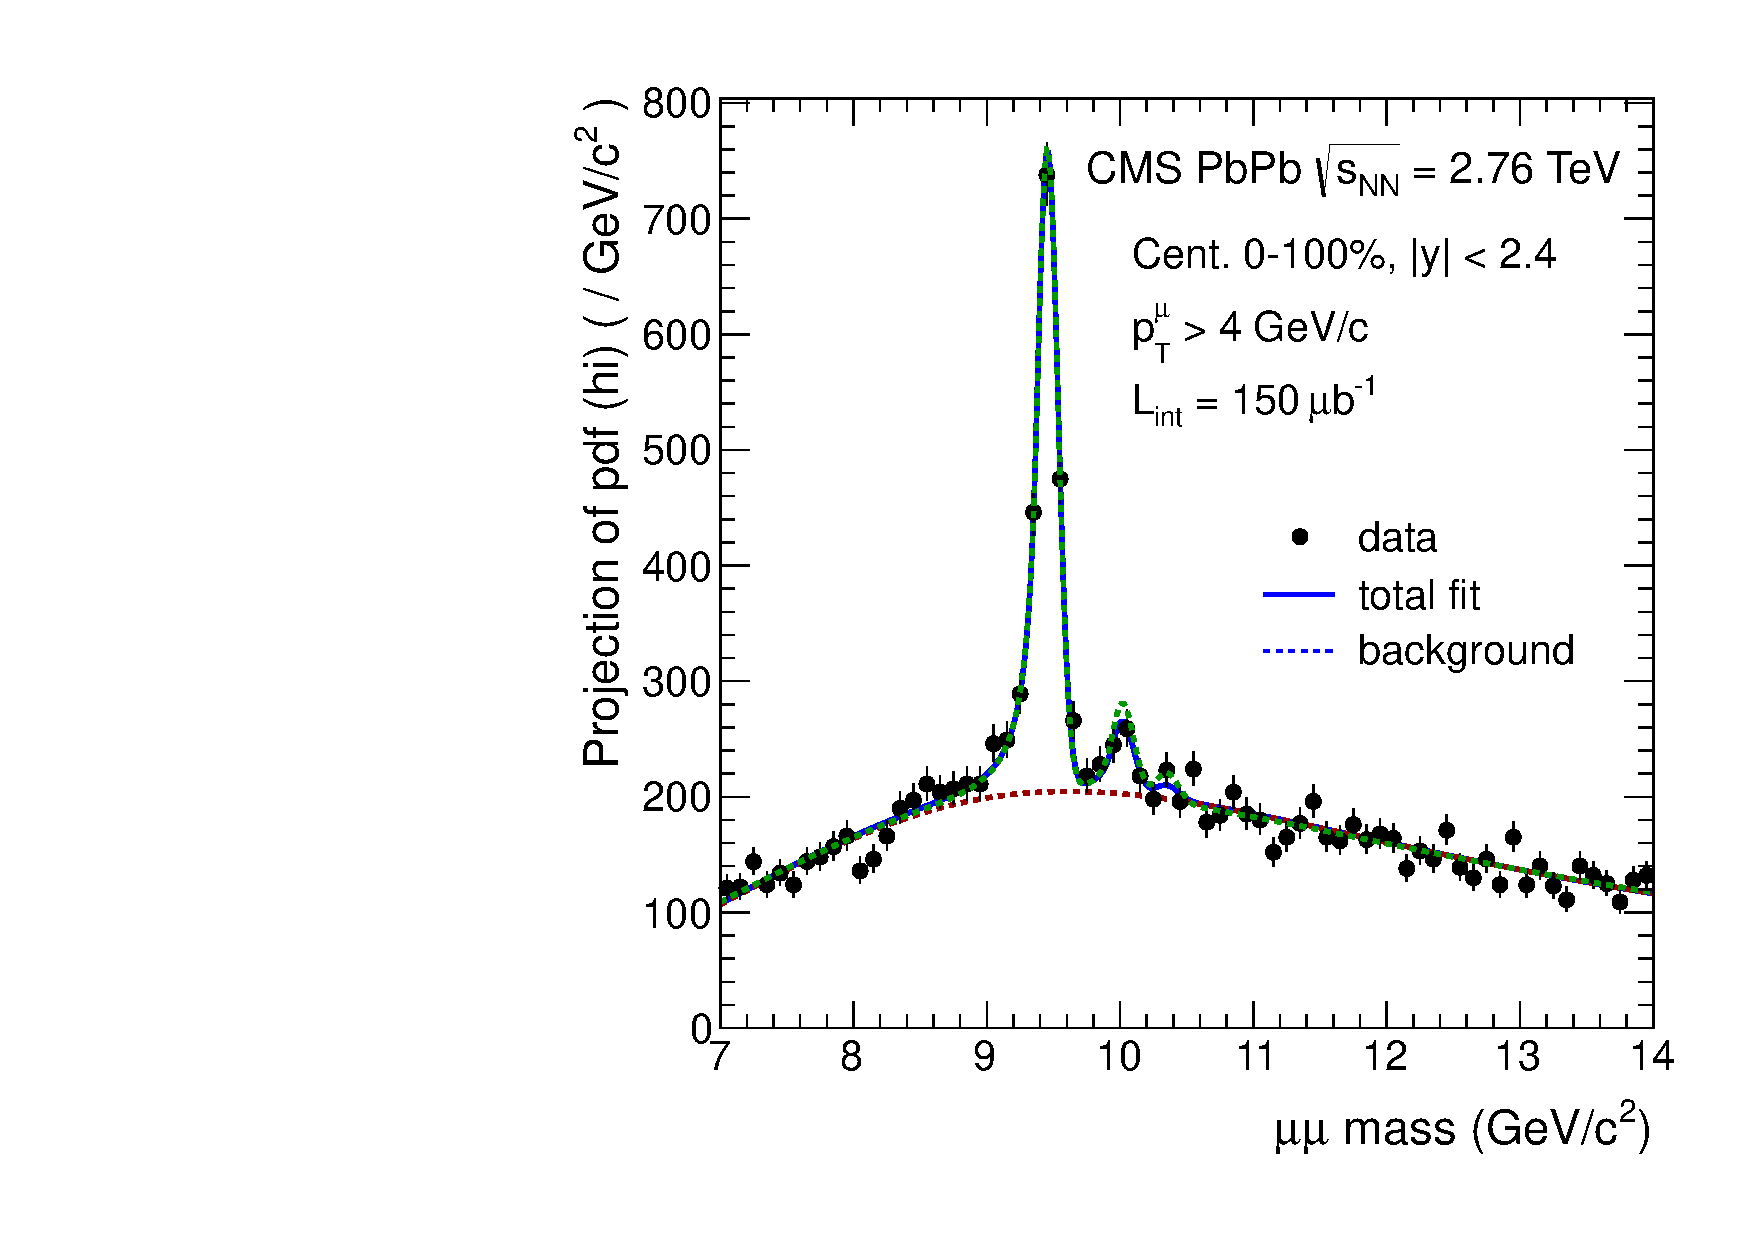
\includegraphics[width=0.45\textwidth]{figures/significance/hiFitY23Ssignificance.pdf}}
\subfigure[\pp data fit projection]{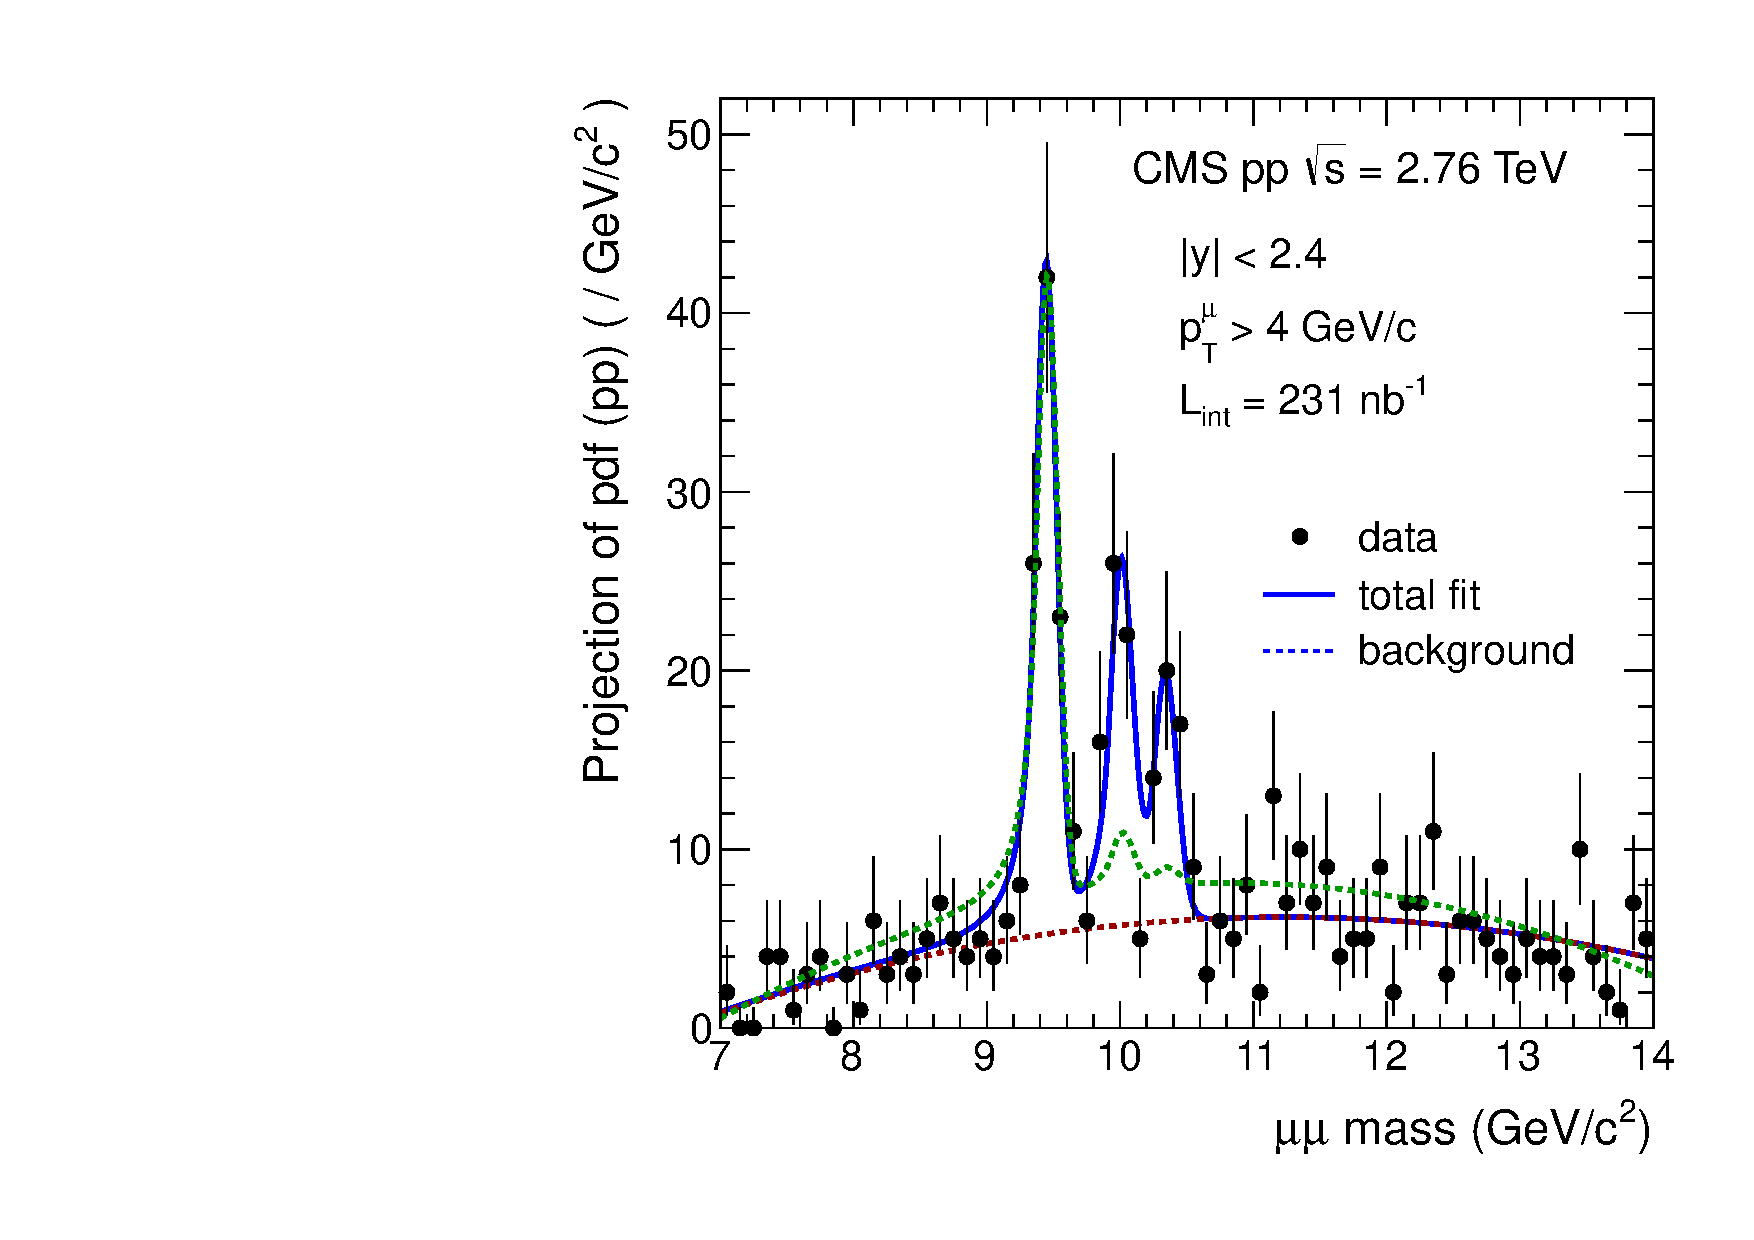
\includegraphics[width=0.45\textwidth]{figures/significance/ppFitY23Ssignificance.pdf}}
\caption{Mass projections of the fit overlaid with the same fit under the assumption of the null hypothesis show in the dashed green curve, used in the estimation of the significance. Null hypothesis: $\PgUb \raa = 1, \PgUc \raa = 1$ }
\label{fig:raa_Y23sSignif}
\end{center}
\end{figure}

\begin{figure}
\begin{center}
\subfigure[\PbPb data fit projection]{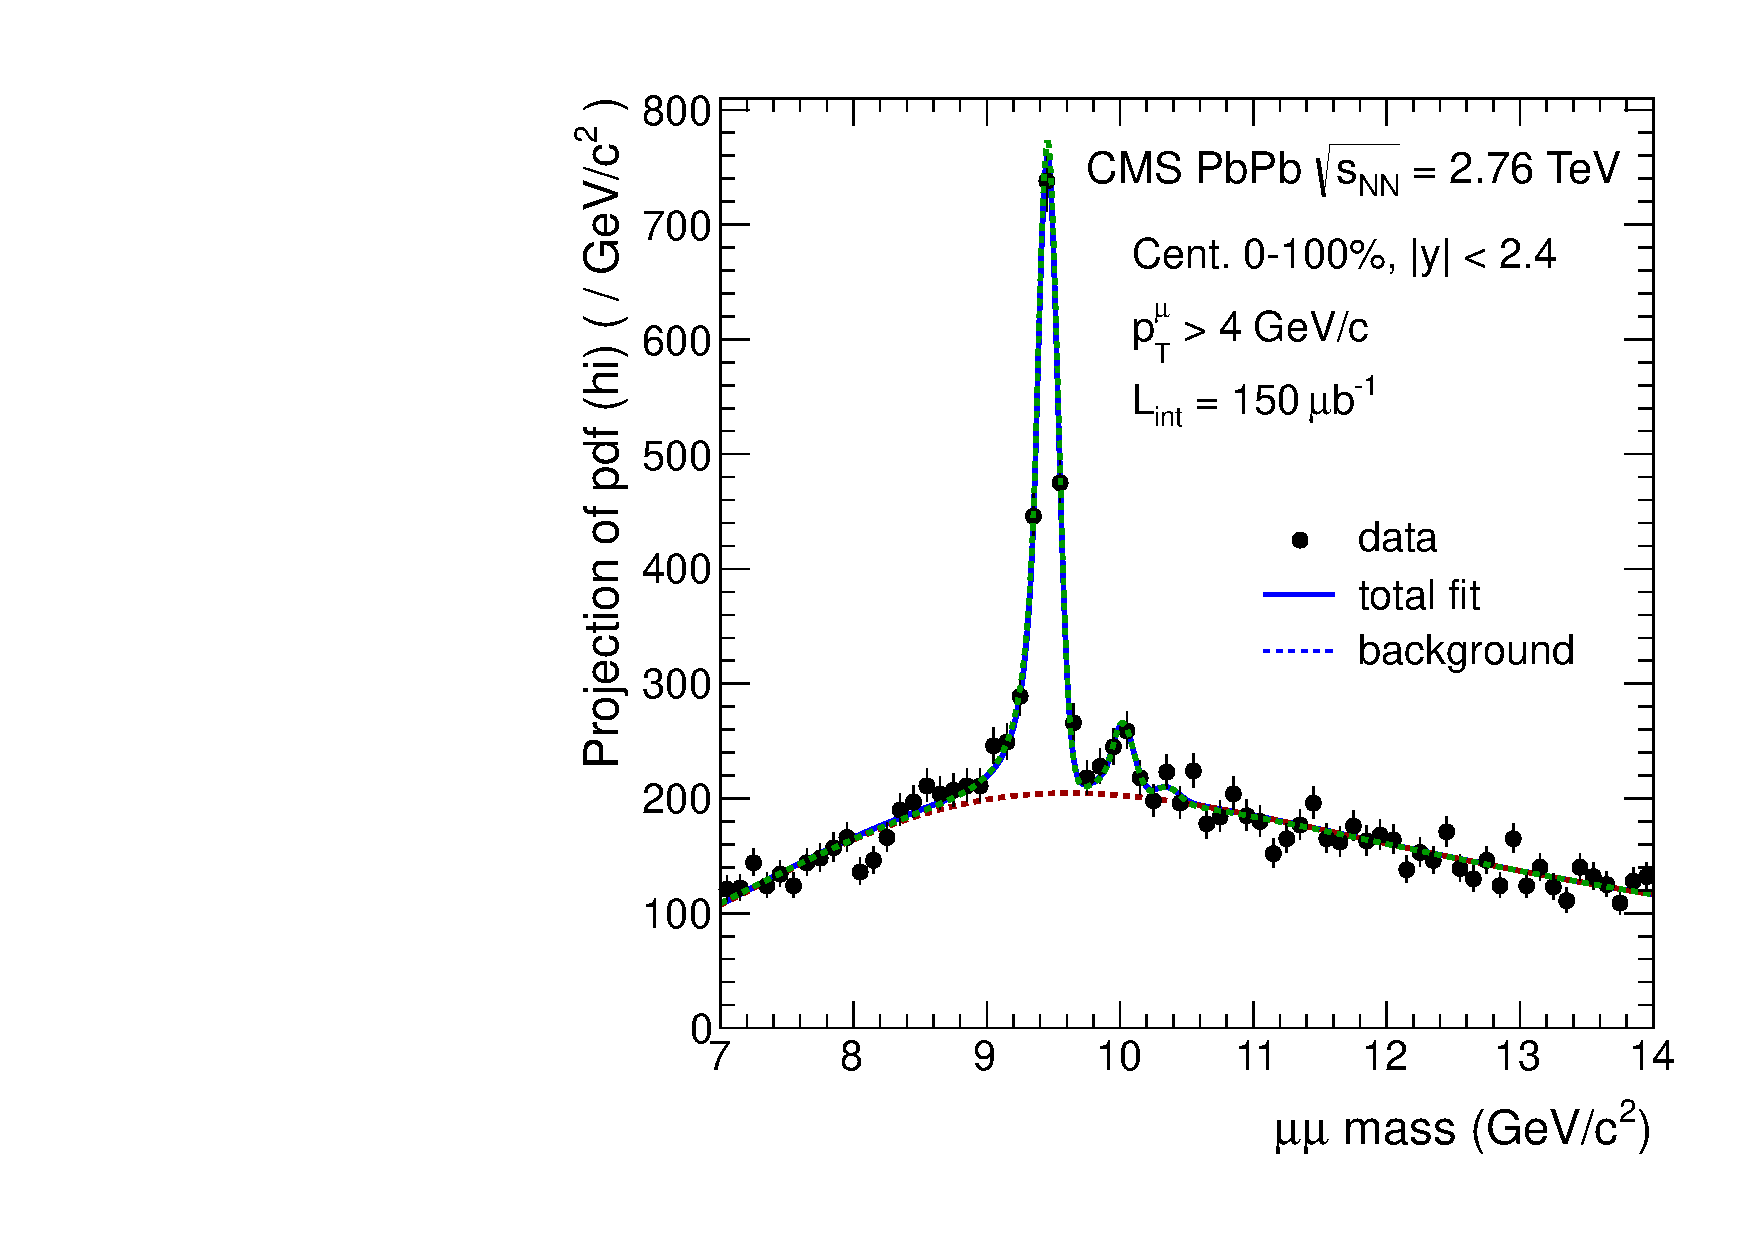
\includegraphics[width=0.45\textwidth]{figures/significance/hiFitY1Ssignificance.pdf}}
\subfigure[\pp data fit projection]{\includegraphics[width=0.45\textwidth]{figures/significance/ppFitY1Ssignificance.pdf}}
\caption{Mass projections of the fit overlaid with the same fit under the assumption of the null hypothesis show in the dashed green curve, used in the estimation of the significance. Null hypothesis: $\PgUa \raa = 1$ }
\label{fig:raa_Y1sSignif}
\end{center}
\end{figure}

\begin{figure}
\begin{center}
\subfigure[\PbPb data fit projection]{\includegraphics[width=0.45\textwidth]{figures/significance/hiFitY1S0-10significance.pdf}}
\subfigure[\pp data fit projection]{\includegraphics[width=0.45\textwidth]{figures/significance/ppFitY1S0-10significance.pdf}}
\caption{Mass projections of the fit overlaid with the same fit under the assumption of the null hypothesis show in the dashed green curve, used in the estimation of the significance. Null hypothesis: $\PgUa \raa = 1$. ($centrality < 10\% $ cut is used for the \PbPb sample.) }
\label{fig:raa_Y1s0-10Signif}
\end{center}
\end{figure}
